
% ******************************* PhD Thesis Template **************************
% Please have a look at the README.md file for info on how to use the template


%Equation 2.1 - define |t| and {t}


%2.6.3 Free-text data: 
%...of which there were four attributes... => a fifth, teleguides, is also included in Table 2.2. Is this attribute used? Also, please include a brief %description of this attribute in he text.


%p55
%On the back of this analysis, a multivariate linear classifier was run on the parameterised data using a balanced dataset, Table 4.2.
%- discuss the results of Table 4.2 in the text.

 
%p57
%Results detailed below are based on the average of five separate runs over a balanced dataset,
%- give the number of training/test instances used in these experiments.


%p56
%The root mean square error reported is relative to the correct output, where 1/0 := frequent /non frequent - unclear if the refers to Table 4.2?


%Equation 4.7: it looks like f_{w, C} denotes the number of documents in which w appears - include a definition of this tern in the text. Also, clarify if TF was normalised by e.g. document length.


%For the experimental results shown in Figures 4.3 and 4.4 (and elsewhere), give details of the number of instances in the dataset and the methodology (e.g. x fold cross validation)


%6.3.1 Word embedding comparison;
%"Training, test, and validation sets were split by user and contained 50%, 25%, and 25% of positive cases respectively, where training and validation sets were balanced, and testing set imbalanced." - give the sizes of the training, validation and test sets (and the same for all experiments). 


%Update legend in Fig 6.10



\documentclass[a4paper,12pt,oneside,times,numbered,print,index,custommargin]{Classes/PhDThesisPSnPDF}

%

% ******************************************************************************
% ******************************* Class Options ********************************
% *********************** See README for more details **************************
% ******************************************************************************

% `a4paper'(The University of Cambridge PhD thesis guidelines recommends a page
% size a4 - default option) or `a5paper': A5 Paper size is also allowed as per
% the Cambridge University Engineering Department guidelines for PhD theses
%
% `11pt' or `12pt'(default): Font Size 10pt is NOT recommended by the University
% guidelines
%
% `oneside' or `twoside'(default): Printing double side (twoside) or single
% side.
%
% `print': Use `print' for print version with appropriate margins and page
% layout. Leaving the options field blank will activate Online version.
%
% `index': For index at the end of the thesis
%
% `draftclassic': For draft mode without loading any images (same as draft in book)
%
% `draft': Special draft mode with line numbers, images, and water mark with
% timestamp and custom text. Position of the text can also be modified.
%
% `abstract': To generate only the title page and abstract page with
% dissertation title and name, to submit to the Student Registry
%
% `chapter`: This option enables only the specified chapter and it's references
%  Useful for review and corrections.
%
% ************************* Custom Page Margins ********************************
%
% `custommargin`: Use `custommargin' in options to activate custom page margins,
% which can be defined in the preamble.tex. Custom margin will override
% print/online margin setup.
%
% *********************** Choosing the Fonts in Class Options ******************
%
% `times' : Times font with math support. (The Cambridge University guidelines
% recommend using times)
%
% `fourier': Utopia Font with Fourier Math font (Font has to be installed)
%            It's a free font.
%
% `customfont': Use `customfont' option in the document class and load the
% package in the preamble.tex
%
% default or leave empty: `Latin Modern' font will be loaded.
%
% ********************** Choosing the Bibliography style ***********************
%
% `authoryear': For author-year citation eg., Krishna (2013)
%
% `numbered': (Default Option) For numbered and sorted citation e.g., [1,5,2]
%
% `custombib': Define your own bibliography style in the `preamble.tex' file.
%              `\RequirePackage[square, sort, numbers, authoryear]{natbib}'.
%              This can be also used to load biblatex instead of natbib
%              (See Preamble)
%
% **************************** Choosing the Page Style *************************
%
% `default (leave empty)': For Page Numbers in Header (Left Even, Right Odd) and
% Chapter Name in Header (Right Even) and Section Name (Left Odd). Blank Footer.
%
% `PageStyleI': Chapter Name next & Page Number on Even Side (Left Even).
% Section Name & Page Number in Header on Odd Side (Right Odd). Footer is empty.
%
% `PageStyleII': Chapter Name on Even Side (Left Even) in Header. Section Number
% and Section Name in Header on Odd Side (Right Odd). Page numbering in footer

% Uncomment to change page style
%\pagestyle{PageStyleII}

% ********************************** Preamble **********************************
% Preamble: Contains packages and user-defined commands and settings
\input{Preamble/preamble}

% ************************ Thesis Information & Meta-data **********************
% Thesis title and author information, refernce file for biblatex
\input{thesis-info}

% ***************************** Abstract Separate ******************************
% To printout only the titlepage and the abstract with the PhD title and the
% author name for submission to the Student Registry, use the `abstract' option in
% the document class.

\ifdefineAbstract
 \pagestyle{empty}
 \includeonly{Declaration/declaration, Abstract/abstract}
\fi



% ***************************** Chapter Mode ***********************************
% The chapter mode allows user to only print particular chapters with references
% Title, Contents, Frontmatter are disabled by default
% Useful option to review a particular chapter or to send it to supervisior.
% To use choose `chapter' option in the document class

\ifdefineChapter
 \includeonly{Chapter3/chapter3}
\fi

% ******************************** Front Matter ********************************
\begin{document}

\frontmatter

\maketitle

\include{Dedication/dedication}
\include{Declaration/declaration}
% ************************** Thesis Acknowledgements **************************

\begin{acknowledgements}      


I would like to acknowledge Science Foundation Ireland for providing the funding that made this work possible. I am also grateful to the Insight Centre for Data Analytics for supplying the resources needed to conduct this research, and a convivial and pleasant environment within which to work.

I would like to thank my supervisor Prof. Tahar Kechadi for giving me the opportunity to do my PhD
and for his valuable guidance and great support throughout this journey.

I wish also to extend my gratitude to Aoife Kavanagh, Dorcas Collier, Margaret Curran, and in particular Michelle Cuniffe, in Caredoc Doctors on Call who all provided invaluable insight into the medical context of the research, and importance of the research question explored in this thesis.     

A very special thanks goes out to my colleagues in University College Dublin, and in particular Ellen Rushe, for their support and friendship during all these years.

\end{acknowledgements}

% ************************** Thesis Abstract *****************************
% Use `abstract' as an option in the document class to print only the titlepage and the abstract.
\begin{abstract}
In an era of “big data”, computational solutions through large-scale machine learning (ML) have provided recourse to problems which previously would have proven very difficult to address. In recent years, ML approaches have been successfully applied to analysis of patient symptom data in the context of disease diagnosis, at least where such data is well codified. However, much of the data present in Electronic Health Records (EHR) are unlikely to prove suitable for classic ML approaches. Furthermore, as scores of data are widely spread across both hospitals and individuals, a decentralised, computationally scalable methodology is a priority.

The focus of this thesis is to develop a method to deliver a framework for decision support in an out-of-hours healthcare provision centre (OOHC). This framework is designed to clean case data, improve the quality of textual features, provide prediction in relation to frequent users of OOHC, and comply with the standard in relation to EHR. These standards relate to data representation, data analysis, and quality of service derived from the data.

Our research is based upon the early identification of a small subsection of patients who are frequent users. These are patients who have underlying conditions which will cause them to repeatedly require medical attention. OOHC act as an ad-hoc delivery of telemedicine and treatment, where interactions occur without recourse to a full medical history of the patient in question. Medical histories, relating to patients contacting an OOHC, may reside in several distinct EHR systems in multiple hospitals or surgeries, which are unavailable to the OOHC in question. As such, although a local solution is a better option for this problem, it follows that the data under investigation is incomplete, heterogeneous, and comprised mostly of noisy textual notes compiled during routine OOHC activities. 

Through a range of machine learning methodologies, the aim of this thesis is to provide the means to identify patient cases, upon initial contact, which are likely to relate to such outliers. In particular, deep learning approaches were adopted in the development of a system of classification of these cases. A further aim of this thesis is to elucidate the discovery of frequent user cases by examining the exact terms which provide strong indication of positive and negative case entries. 


\end{abstract}

% ************************** Thesis Abstract *****************************
% Use `abstract' as an option in the document class to print only the titlepage and the abstract.
\begin{abstract2}

The following work has been published as part of the research described in this thesis.

 \section*{Papers}
  \begin{enumerate}
  \item Wallace, Duncan, and Tahar Kechadi. "Prediction of Frequent Out-Of-Hours’ Medical Use." ECML PKDD 2019 Workshops: Nemesis 2019, UrbReas 2019, SoGood 2019, IWAISe 2019, and Green Data Mining 2019,  Würzburg, Germany, September 16-20, 2019, Proceedings.
  \item Wallace, Duncan, and Tahar Kechadi. "Outlier Detection in Health Record Free-Text Using Deep Learning" 2019 41st Annual International Conference of the IEEE Engineering in Medicine and Biology Society (EMBC). Berlin, Germany, July 23-27, 2019.
   \item Wallace, Duncan, and Tahar Kechadi. "Analysis of EHR Free-text Data with Supervised Deep Neural Networks." CSCE'18: The 2018 World Congress in Computer Science, Computer Engineering \& Applied Computing, Las Vegas, Nevada, USA, 30 July-02 August 2018.
  \item Wallace, Duncan, and Tahar Kechadi. "Abbreviation and Acronym Identification and Expansion Within Medical Health Records." The 9th International Conference on e-Health, Lisbon, Portugal, July 20-22. IADIS, 2017.
  \item  Wallace, Duncan, and Tahar Kechadi. "Retrieval and Clustering of Medicines Within Healthcare Data Records." Proceedings of the International Conference on Big Data and Advanced Wireless Technologies. ACM, November 10-11,  2016.
  \end{enumerate}
  \section*{Posters}
  \begin{enumerate}
  \item Wallace, Duncan, and Tahar Kechadi. "Frequent attender Classification through Electronic Health Record Analysis" Science and Information Computing Conference 2019, London, United Kingdom. 16-17 July, 2019. 
  \end{enumerate}
  
%  @inproceedings{ibrahim2018optimal,
%  title={Optimal Moore Neighborhood Approach of Cellular Automaton Based Pedestrian Movement: A Case Study on the Closed Area},
%  author={Ibrahim, Najihah and Hassan, Fadratul Hafinaz},
%  booktitle={Science and Information Conference},
%  pages={57--71},
%  year={2018},
%  organization={Springer}
%}
  
 
% @inproceedings{paudice2018label,
%  title={Label sanitization against label flipping poisoning attacks},
%  author={Paudice, Andrea and Mu{\~n}oz-Gonz{\'a}lez, Luis and Lupu, Emil C},
%  booktitle={Joint European Conference on Machine Learning and Knowledge Discovery in Databases},
%  pages={5--15},
%  year={2018},
%  organization={Springer}
%}

%@inproceedings{huang2018roast,
%  title={ROAST: an open-source, fully-automated, realistic volumetric-approach-based simulator for TES},
%  author={Huang, Yu and Datta, Abhishek and Bikson, Marom and Parra, Lucas C},
%  booktitle={2018 40th Annual International Conference of the IEEE Engineering in Medicine and Biology %Society (EMBC)},
%  pages={3072--3075},
%  year={2018},
%  organization={IEEE}
%} 


%@inproceedings{wallace2019outlier,
% title={Outlier Detection in Health Record Free-Text Using Deep Learning},
%  booktitle={2019 41st Annual International Conference of the IEEE Engineering in Medicine and Biology Society (EMBC)},
%  pages={3072--3075},
%  year={2019},
%  organization={IEEE}
%}


\end{abstract2}

%
\begin{publications} 

Oh hey

\nobibliography{ref}
  \bibliographystyle{unsrt}

  \section*{Publications}
  \begin{enumerate}
    \item \bibentry{salton1988term}
    \item \bibentry{ramos2003using}
  \end{enumerate}
  
\end{publications}
% *********************** Adding TOC and List of Figures ***********************

\tableofcontents

\listoffigures

\listoftables

% \printnomenclature[space] space can be set as 2em between symbol and description
%\printnomenclature[3em]

% abbreviations:






\printnomenclature


% ******************************** Main Matter *********************************
\mainmatter


\chapter{Introduction}
%\setcounter{page}{1}

\renewcommand\nomgroup[1]{%
  \item[\bfseries
  \ifstrequal{#1}{A}{Physics Constants}{%
  \ifstrequal{#1}{B}{Number Sets}{%
  \ifstrequal{#1}{C}{Other Symbols}{}}}%
]}

\nomenclature[1]{ML}{Machine Learning}
\nomenclature[1]{DM}{Data Mining}
%\nomenclature[1]{CFD}{Computational Fluid Dynamics}
\nomenclature[1]{OOHC}{Out-Of-Hours health Care} 
\nomenclature[1]{A\&E}{Accident and Emergency} 
\nomenclature[1]{FA}{Frequent Attender} 
\nomenclature[1]{GP}{General Practitioner} 
\nomenclature[1]{EHR}{Electronic Health Record} 
\nomenclature[1]{DL}{Deep Learning} 


 As the volume, variety, and velocity of clinical data grow, there is increasing need for computational models to effectively mine these data. Machine learning is widely known for its successful industrial applications. Increased adoption of machine learning (ML) in competitive industry largely stems from the increased efficiency offered by knowledge extraction. Research concerning the potential benefit of disease detection has, in particular, gained impetus in recent years. 
 
 
  %We are motivated by problems in the medical domain that can be formulated as binary supervised classification problems, the application of which in this case is the prediction of patients who will have high level of contact with health care providers. We hope through these means the provision of medical solutions that are personalised and less costly may be developed, and finally, improve the quality of care for such patients.
 
 Traditional health care models of medical treatment, limited to a single option has provided somewhat procrustean solutions to patient needs, are slowly giving way to concepts concerning both personalised health care and community based intervention \cite{mahato2017paper}.
 Nowadays, the development of decentralised regional programmes is increasing the avenues of treatment available for patients \cite{iyengar2016role}. 

The thesis of this research is that through the mining of Electronic Medical Records containing mixed types of data, and extracting patterns from the processed data, patients can be successfully categorised through means of supervised machine learning early in their engagement with health care providers. This categorisation has quite narrow factors: the aim of which is to provide recourse to patients that are less suitable to the health care provider being examined in the course of this research; specifically, an out-of-hours health care cooperative.


 


\section{Motivation}

Frequent use of helplines, emergency departments, and primary care is heavily associated with serious medical conditions, the requirements of which are often not being met in the recourse offered to these patients \cite{daniels2018better}.  Emergency and out-of hours primary care prove to be ill adapted at treating many of these patients. Although these facilities are adept at handling acute episodes, by necessity these healthcare providers are limited to the short-term, superficial treatment that will not engage with the primary issues facing this cohort.  A growing body of research has suggested the creation of a specific arm of healthcare provision, featuring staff specifically trained to treat frequent users cases \cite{malins2016cognitive,buja2015determines}. Moreover, strategies need to be developed to attempt to tackle underlying issues which are bringing these types of patients into contact with healthcare provision. 

General Practitioners (GPs) are often the first point of contact for most people when they feel unwell, and play a crucial role as primary care in the country’s health care system. While the majority of appointments with a GP are made during the working week, a number of GP Out-of-Hours services also exist for people who require medical treatment when GP practices are closed, such as in the evening, at weekends, and on public holidays. GP Out-of-Hours services are part of a larger network of unscheduled care providers which also includes emergency ambulances and Accident and Emergency (A\&E) Departments. 

 
 The context of this research is treatment provided by an out-of-hours health-care cooperative (OOHC\index{Out-of-hours Health Care}). OOHC\index{Out-of-hours Health Care}  act as an intermediary between GP surgeries and hospital A\&E departments. A major reason for the development of OOHC\index{Out-of-hours Health Care} was to reduce public dependence on hospital emergency departments during periods when a patient's GP may not be available. OOHC\index{Out-of-hours Health Care} are unsuited to more serious complaints, and are not meant to act as a substitution for secondary or tertiary health care. High level out-of-hours health-care management in the form of cooperatives is becoming  an increasingly common means of primary health care provision. Electronic Helath Records (EHRs) are habitually used in primary care such as this for the recording of patient data \cite{michiels2017influenza}.

Out-of-hours health care is ad-hoc. Unlike scheduled medical treatment, the availability of patient data is usually limited to whatever in-house Electronic Health Record system the institution in question is operating. As such, medical histories, relating to people contacting an out of hours health care organisation, may reside in several distinct EHR systems in multiple hospitals or surgeries which may be unavailable to the out-of-hours care provider in question \cite{warner2019s}. This often results in a wide dispersal of health care data relating to individuals, thereby necessitating the development of decentralised solutions when considering the treatment of such data.

Electronic Health Records are typically designed to electronically document all information that is administratively and clinically relevant in a patient's use of a health care facility. EHR\index{Electronic Health Record} are designed as a way to standardise data collection, storage, and usage. Worldwide EHR\index{Electronic Health Record} usage has grown rapidly in the last two decades, generating vast quantities of data in departments where they are routinely used \cite{safran2014reuse}. In recent years, ML approaches in the medical domain have been successfully applied to the analysis of patient symptom data in the context of disease diagnosis, at least where such data is well codified. However, much of the data present in EHRs\index{Electronic Health Record} is unlikely to prove suitable for classic ML approaches \cite{harutyunyan2017multitask}. In particular, while the use of free (or unstructured) text for clinical notes presents significant analytical opportunities, it also poses unique difficulties such as high dimensionality, noise, and contextual sensitivity. 

 
 
 This thesis provides an overview of an approach to develop a framework of patient classification in the environment of EHRs\index{Electronic Health Record} where data is heterogeneous, incomplete (containing missing values), and noisy. This thesis focuses on a means to develop canonisation of data contained within the narrative-based free-text\index{free-text} notes of patients' health care data records, the processing of patient textual data to improve feature quality, and the classification of patient cases using deep learning techniques. 
 
 Specifically, this research is based upon the early identification of patients who have underlying conditions which will cause them to repeatedly require medical attention, far beyond what would be witnessed in the general population. These patients are a poor match to the services provided by telemedical\index{telemedicine} out-of-hours organisations, which are predominantly designed to treat acute and emergency cases rather than chronic illnesses. Frequent users take up approximately 4\% of the working hours of the organisation under consideration: an overwhelmingly disproportionate figure, as such patients account for only 0.04\%  of the population served. 
 % On average take up x * more time than non-FA patients
 
 The equipment, software, and practices used in the organisation under investigation represent a standard mode of delivery within Ireland, and closely mirror that found throughout the United Kingdom in the provision of equivalent services. Nonetheless, we aim, in the course of this thesis, to a develop a methodology for patient classification that will not be circumscribed to the specific systems or data storage structures employed by the organisation in question, but would provide a solid basis for generalisation in the context of other hypothetical EHR\index{Electronic Health Record} systems.  



\section{Problem Statement}
\label{section:problem-statement}

It would be useful for OOHC\index{Out-of-hours Health Care}, such as the cooperative under investigation, to be able to have a \textit{prima facie} detection of patients likely to become frequent users. This ability, however, is not only outside the scope of call operators' responsibilities, but would prove challenging for a human to accurately predict. This difficulty in detection is not merely due to frequent user patients being exceptional cases, but even within this cohort there is significant variance both in the demographic, and pathographic information relating to these patients. 

Further challenges in the detection of these patients include the nominal complaint of frequent users (and apparent cause of their contacting the OOHC\index{Out-of-hours Health Care} organisation in the first place) being separate from underlying chronic issues. This inadvertently acts to obfuscate the more significant problems relating to these patients. Furthermore, these nominal complaints are liable to be different (in either detail or magnitude) with each call. 

While patient medical histories are part and parcel of all EHR systems, each time a patient is treated by triage this is handled as a separate case. In the organisation in question, call handlers would have to manually search the company's database to be provided with information relating to previous encounters. Demographic and contact information are the only exceptions to this, as the structured information in these fields are used to populate current cases as a matter of course.

The aim of this thesis is to provide the means to predict potential frequent user patients upon initial contact with the OOHC\index{Out-of-hours Health Care} organisation. To this end the thesis must provide a formal definition, with respect to the OOHC\index{Out-of-hours Health Care} organisation in question, of what constitutes \hl{a} frequent user, an episode of care, and a case record. The data discussed within this thesis relates to a subsection of this organisation, covering a distinct geographical area in Ireland for the year 2014.

\newpage

\section{Objectives}
\label{section:thesis-objectives}

Objectives for this research include:

\begin{enumerate}
  \item The capacity to process raw output from medical systems in such a manner that they can be used in a research capacity. This includes automated anonymisation, extraction, and normalisation of data stored in our collaborator's systems. These data should be analysed to discover the broad characteristics of both the general population, and outlier cases that are the subject of the thesis' investigation. The identification of features which may be useful in predictive analytics must also be performed.

  \item The development of machine learning techniques in the context of the domain specific natural language that features within case information. We endeavour to create means to disambiguate overloaded signifiers that, in their unprocessed form,  result in polysemy in the clinical notes. In particular, the treatment of potentially high value terms, that may be recorded in abbreviated or acronym form is a key objective in the preprocessing of this data. Feature reduction in relation to such contractions, and also the abstraction of medical identifiers, are additional processes to be conducted in this stage.

% You say decentralised a lot


  \item This thesis will also outline the generation of a data analysis solution with respect to OOHC\index{Out-of-hours Health Care} patient medical informatics. Data relating to patients is incomplete, as patient information which resides with patients' general practitioners or in hospitals is not available to the OOHC\index{Out-of-hours Health Care} in question. As such, case data within the OOHC\index{Out-of-hours Health Care} often form little more than partial snapshots into a patient's medical history. The incomplete nature of patient medical histories is a typical feature of OOHC\index{Out-of-hours Health Care} \cite{yadav2018mining,moskow2015identifying,petersen2019health}. 

  \item As there exist several forms that the unstructured data can take, and also several deep learning architectures which can be used for the purpose of classification, an appropriate configuration will have to be derived.  Hyperparameter optimisation, and other measures to further improve accuracy within the chosen configuration will be explored. Subsequently, an inspection of what features perform best in terms of case classification will be executed, and the implications this may pose in relation to FA patients discussed.
\end{enumerate}


%Further objectives include the integration of structured and unstructured data,  

\section{Contributions}

This thesis makes the following contributions 

\begin{enumerate}
  \item \textbf{Quality of services and tools:} A framework which improves upon the state-of-the-art capacity to predict frequent user patients in unseen, real world data.
  \item \textbf{Data quality:} Description of novel means to process medical text - solving extant issues concerning aberrant or inconsistent methods of recording medical terms in unstructured text. The methodology we adopted to solve these problems allows the approach described to be applied in relation to any English based free-text\index{free-text}.
  \item \textbf{Data analytics and mining techniques:} An advance in the understanding of Deep Learning with respect to natural language in the medical domain; providing an analysis of competing approaches which have hitherto not been approached.
\end{enumerate}



\section{Thesis Structure}



To achieve the objectives outlined above, the remainder of this thesis has been
organised as follows:

\textbf{Chapter 2} examines the context within which this research takes place and the bearing this has upon data-mining (DM) and ML approaches, the problem domain, and some of the research constraints. The methods used to compose the dataset that is treated as part of this dissertation will be discussed, followed by a detailed examination of the corpus; giving an oversight of the potential value provided by the different aspects of the dataset. This chapter is designed to both motivate and define the problem central to this thesis. 


\textbf{Chapter 3} provides a description of the extant state of the art research in our problem domain, and some of the methodologies that have been developed to treat medical data similar to that being examined in this thesis. Literature concerning both high-use prediction and medical text processing will be discussed at length (relating to this thesis' classification objective and main source of features respectively). Difficulties of natural language processing as they relate to a medical context will be examined in this chapter.

% of the environment from which our data originates and the significance this posed, both in terms of the motivation for or research, and the issues which were encountered when attempting to develop our solution.

\textbf{Chapter 4}  develops a proof-of-concept, and analysis of the competing ML approaches available for classifying patient cases. Looking at the types of data discussed in Chapter 2, this chapter looks at potential features for classification. This chapter also outlines the system for classifying patients to be developed - detailing both the challenges and proposed solutions when addressing the issues raised in earlier chapters. 

\textbf{Chapter 5} establishes data transformation methodologies in order to improve the quality of data being analysed in depth in this chapter:  focusing on normalisation of data, medical transformation, and contraction clustering. The theory, methodologies, and results from these processes will be discussed at length in this chapter.

\textbf{Chapter 6} discusses the means of implementing our solution, focusing on the development of optimum neural network architecture for case classification. This chapter discusses the possible architecture and data types that could be used for the classification of patient cases, before resolving the best combination of such for achieving this goal. The chapter discusses gating techniques, different means of generating word embeddings, and the impact of dimensionality and feature length on classification performance. Finally this chapter provides an explanation for the performance of the system that has been developed.

\textbf{Chapter 7} reviews the thesis, provides some details relating to future work, and discusses ethical implications for this work.




%data mart 

%:1.  How to discover which features are most successful in identifying problem patients.2.  How  to  determine  the  importance  of  different  contextual  elements  in  relation  totextual features.3.  The extent to which features can be deemed independent of one another11
%4.  The threshold of cases (i.e.  data) about individuals that is required before a pre-diction can be arrived at.Of  particular  importance  in  the  choice  of  algorithm  is  the  manner  in  which  theissue  of  overfitting  is  addressed.   High  demand  patients  are  outliers  by  their  nature:representing less than 1\% of patients within the corpus.  Although high demand patientshave a significantly higher than average volume of cases, without significant investmentthe limited cohort is liable to produce bias within a supervised learning environment.


\chapter{Background \& Medicinal Dataset}
\label{chpt:background}
%\setcounter{page}{1}
\nomenclature[1]{HSE}{Health Service Executive} 
\nomenclature[1]{HIS}{Health Information System} 
\nomenclature[1]{Caredoc}{Carlow Emergency Doctors on Call}
\nomenclature[1]{NLP}{Natural Language Processing}
\nomenclature[1]{ED}{Emergency Departments}
\nomenclature[1]{FC}{Frequent Caller}

\nomenclature[1]{ICD}{International Classification of Diseases}
\nomenclature[1]{FTN}{Free-text notes}
\nomenclature[1]{HIPE}{Hospital In-Patient Enquiry}
\nomenclature[1]{SNOMED}{Systematized Nomenclature of Medicine}
\nomenclature[1]{SCOWL}{Spell Checker Oriented Word Lists}
\nomenclature[1]{UMLS}{Unified Medical Language System}
\nomenclature[1]{GMS}{General Medical Services} 
\nomenclature[1]{NER}{Named Entity Recognition} 
\nomenclature[1]{AUC}{Area Under Curve} 
\nomenclature[1]{ROC}{Receiver Operating Characteristic} 
\nomenclature[1]{CDSS}{Clinical Decision Support Systems} 
\nomenclature[1]{NHS}{National Health Service} 

\section{Introduction}


This section describes the relevant background for the research described in this thesis in three separate parts: (i) Out-Of-Hours Healthcare, (ii) Electronic Health Records, and (iii) Frequent Users of primary health care. This background helps motivate the thesis problem, inform the reader about what resources are available in the course of the thesis' investigation, and establish some of the limitations within which the research has to work. 


\section{Out-Of-Hours Health-Care}
\label{Out-Of-Hours_Health-Care}

%Out-of-hours health care provision (OOHC\index{Out-of-hours Health Care}) act as an ad-hoc delivery of triage and treatment, where interactions occur without recourse to a full medical history of the patient in question. Medical histories, relating to patients contacting an OOHC\index{Out-of-hours Health Care}, may reside in several distinct Electronic Health Record (EHR\index{Electronic Health Record}) systems in multiple hospitals or surgeries, which are unavailable to the OOHC\index{Out-of-hours Health Care} in question. As such, although a local solution is optimal for this problem, it follows that the data under investigation is incomplete, heterogeneous, and comprised mostly of noisy textual notes compiled during routine OOHC\index{Out-of-hours Health Care} activities. 

``Out of Hours'' refers to periods of the week where GPs (or family physicians) would be unavailable. \hl{At least in the Irish context under consideration}, these typically relate to periods outside of the standard working day (for instance  periods between 18.00 and 08.00 during weekdays, and the entirely of weekends and public holidays). People telephoning their GP surgeries may be automatically redirected to call operators working on behalf of an OOHC\index{Out-of-hours Health Care} cooperative, depending on what part of the country they are living in. 

OOHC\index{Out-of-hours Health Care} cooperatives are a relatively modern health care delivery system, forming a hybridisation of traditional primary care and telemedicine.  Similar to the structure adopted by the United Kingdom's National Health Service (NHS), % https://www.independent.ie/irish-news/caredoc-irelands-flying-doctors-26133491.html
out-of-hours care in Ireland features a plethora of services, including walk-in centres, out-of-hours centres, telephone consultation, and the emergency department (A\&E) \cite{coombes2016fix}. The complicated pathway that data can take with respect to the organisation under consideration can be seen in Figure \ref{fig:dia0}. 

\begin{figure}[h]
   \centering
   \begin{tabular}{@{}c@{\hspace{.5cm}}c@{}}
 \includegraphics[page=7,width=1.0\textwidth]{Figs/data-flow2.pdf} & 
   \end{tabular}
 \caption{Data flow, agency interaction, and different system usage in relation to OOHC\index{Out-of-hours Health Care} under consideration.}
 \label{fig:dia0}
\end{figure}


The Health Services Executive (HSE) is responsible for the provision of all of Ireland's public health services, both in hospitals and communities across the country. Carlow Emergency Doctors on Call (Caredoc) is a non-profit health care provider, which, through service level arrangements with the HSE, provides OOHC\index{Out-of-hours Health Care} services to patients \cite{cunniffe2016developing}.  The HSE tenders for new services as required, and over the last number of years, Caredoc\index{Caredoc} has been successful in its bids for such contracts \cite{cunniffe2016developing}. 

Figure \ref{fig:dia0} details the flow of both user interaction (in black) and of information (in blue) throughout possible engagement scenarios with Caredoc\index{Caredoc}'s organisation. The scope of Caredoc\index{Caredoc}'s integrated care model is nominally quite broad, but fundamentally it is underpinned by its operation of a call centre which provides the hub for out-of-hours care for quite a wide geographical area. This call centre, dealing directly with patients (labelled \textit{A} in Figure \ref{fig:dia0}) or through a third party calling on the behalf of patients, form the bulk of the information pertaining to patients, held by the organisation. It has been envisioned since its inculcation, that nurse/doctor operated phones, providing both advice and triage, would reduce the burden on other areas of the health service during out-of-hours operation \cite{khistriya2010nhs}.




Caredoc\index{Caredoc} uses a very complicated healthcare software system for the purposes of providing an extensive telemedicine\index{telemedicine} capacity. Nurses operate the phones (\textit{B}) and provide triage, whereupon the caller may be given advice by the nurse, or directed to a doctor who will give advice by phone. Alternatively, the result of the triage may be that a general practitioner locum is sent to conduct a home visit (\textit{C}), or the patient may be asked to visit one of the treatment centres under Caredoc\index{Caredoc}'s management (\textit{D}). Some combination of the above is also possible.  

Regardless of the outcome, the information relating to the call, and any action taking place under Caredoc\index{Caredoc}'s auspices gets recorded in the Electronic Patient Records (\textit{E}), managed by the organisation. If the patient in question was originally redirected from another institution, this information is passed onto these respective organisation. 

\begin{figure}[ht]
   \centering
   \begin{tabular}{@{}c@{\hspace{.2cm}}c@{}}
 \includegraphics[page=3,width=1.0\textwidth]{nightingale.png} & 
   \end{tabular}
 \caption{CDSS\index{Clinical Decision Support Systems} interface used by OOHC\index{Out-of-hours Health Care} phone operators}
 \label{fig:screen2}
\end{figure}



However, the telemedicine\index{telemedicine} and triage described above is not diagnostic in nature. Numerous OOHC\index{Out-of-hours Health Care} take advantage of software for clinical decision making, typically known as clinical decision support systems (CDSS\index{Clinical Decision Support Systems}), and Caredoc\index{Caredoc} is no exception in this regard \cite{kasem2017exploring}. \hl{The software in question, known as Nightingale, is visible in Figure} \ref{fig:screen2}.  CDSS\index{Clinical Decision Support Systems} take in symptoms input by nurses, and make suggestions about the types of conditions the patient may be suffering from. This software is useful is narrowing down the scope of what nurses should consider when dealing with patients, but neither the values input by phone operators, nor the suggested comorbidities derived by the CDSS\index{Clinical Decision Support Systems} are actually recorded.  

The patient records treated in this research may be presented \emph{in media res}, as patients will have had prior interaction with healthcare that is not recorded, and indeed may have possible further  interaction with health infrastructure, that is likewise unavailable within the scope of this project\footnote{as this information is available to neither Caredoc\index{Caredoc}, nor this research}. The data flow within Caredoc\index{Caredoc} is independent of any information relating to patients which may exist in health records in other health care organisations (such as in hospitals, or with the patient's own GP). While Caredoc\index{Caredoc} will transfer data to a patient's GP (or public health nurse, where appropriate) (\textit{F}), the reverse is not true. Consequently, if diagnoses are made in relation to these patients in subsequent analysis, these diagnoses are unlikely to feature within the data possessed by the co-op, unless specifically mentioned by the patient in a potential subsequent interaction between the co-op and the patient. As this information is not available to Caredoc\index{Caredoc}, it thus unavailable to the research described in this thesis.

Consequently, data relating to patients often form little more than snapshots. The incomplete nature of patient medical histories is a typical feature of OOHC\index{Out-of-hours Health Care} \cite{aldosari2017patients}. A decentralised solution with respect to OOHC\index{Out-of-hours Health Care} patient medical informatics is thus a key motivation of this research. 

The software used to record each of episode of care is Ad Astra\index{Ad Astra}\texttrademark \cite{adastra}. Most of the OOHC\index{Out-of-hours Health Care} in both Ireland and the UK use this particular software (or at least some version of it) \cite{natreview}. The limitations of this software are important in terms of the challenges that were present with respect to the data. This chapter will cover some of the preexisting issues relating to data storage that had to be addressed in the scope of our research. 

%system under investigation did not use primary keys to identify patients, and episodes of care were all recorded in unstructured text.~\cite{adastra} [fixbib]
 
 \section{Electronic Health Records}

Electronic Health Records\index{Electronic Health Record}, Electronic Medical Records, and Personal Health Records relate to the digital storage of patient information. These three terms are not quite synonymous, although depending on context they may be used interchangeably. The distinction between the terms relates to how comprehensive the medical information relating to a patient is, with Electronic Medical Records typically relating to information stored in a single institution, Electronic Health Records typically relating to information shared between institutions, and Personal Health Records typically relating to all recorded information about a patient \cite{heart2017review}. However, as is common in nomenclature relating to health care management, usage is not particularly consistent between different researchers. For our purposes we will consider the data system managed by Caredoc\index{Caredoc} to be an Electronic Health Record, as it contains information shared between different organisations, but provides a very disjointed and incomplete record relating to individual patients.  

The concept of an Electronic Health Records was set out in order to close the gap between institution-specific patient data and a comprehensive, longitudinal collection of the patient's health data \cite{quaglio2016health}. During the early adoption of EHR\index{Electronic Health Record}, recording increasingly tended to reflect institutional priorities. These priorities were largely shaped by the social contexts of medical practice, but institutional priorities could only be achievable if there was standardisation in relation to the methods of recording data within the institution's EHR\index{Electronic Health Record}  \cite{doi:10.1111/nup.12112}\hl{.} The consequence of this use of EHR\index{Electronic Health Record} was a de‐emphasis on the patient's narrative as a source of input into the health record, but instead a shift towards representing the patient as a set of data points or metrics \cite{doi:10.1111/nup.12112}. EHR\index{Electronic Health Record}-like systems and e-prescription are priorities in various EU e-Health Action Plan and in the policies of several Member States ( 27 and 22 EU countries respectively). However, the general political commitment to these e-health fields is at different stages of implementation across countries \cite{stroetmann2011european}. Overall, on average, 77.4\% of GPs across Europe store patient consultations in some form of EHR\index{Electronic Health Record} \cite{de2015basic}.

While the digital recording of patient data has been embraced by many countries due to the potential benefits such a policy poses to cost effectiveness of health care provision, accuracy of treatment for patients, and research \cite{peckham2016electronic}, there are a number of extant problems that are common among EHR\index{Electronic Health Record} implementation. Most EHR\index{Electronic Health Record} systems used in health centres are proprietary systems built with different architectures, business rules, information technologies and models, in addition to incompatible clinical terminology. These facts hinder the interoperability among the Health Information Systems (HIS), making it difficult for health professionals to provide continuity of care \cite{gomes2018marcia}.


One significant regional difference between digital medical records in the United States, and those operated in both Ireland and the United Kingdom, is that patient billing forms a large part of the purpose of data recording in the United States, thereby having an impact on the manner in which data is recorded \cite{alpert2019electronic}. Another distinctive regional attribute is that before recent legislative change \cite{kelleher2015privacy}, there has been no legal basis within Ireland for national identifiers for patients. As pointed out by Leonidas et al., legal and political considerations, as well as diverse local complications have made significant long-term hurdles to national implementations of EHR\index{Electronic Health Record} \cite{fragidis2018implementation}. In particular, bottom-up approaches whereby individual hospitals and institutions decide themselves upon what HIS to use, as is typical in the United States, is likely to make interoperability between different institutions' EHR\index{Electronic Health Record} an ongoing challenge \cite{fragidis2018implementation}. The absence of national identifier for patients in Ireland, coupled with legal restrictions and differences in institutional HIS has precluded consistent sharing of patient data between health care services in Ireland. 





\section{Information Systems \\ and Recording Practices}

Electronic Health Records used in the operation of out-of-hours cooperatives are composed of both structured and free-text\index{free-text} clinical notes. However, knowledge discovery currently has very limited application in Caredoc\index{Caredoc}. Identification of patterns within this data, at either a population or individual level, is limited to shallow treatment and narrow parameterisation (i.e. relatively simple queries) \cite{cunniffe2016developing,adastra}. The software used by Caredoc\index{Caredoc}  has a number of structural flaws, such as a lack of primary key for patients, redundant data fields, noisy input, and significant software bugs, which is partially responsible for the restricted scope with which Caredoc\index{Caredoc} can treat its data. 

\begin{figure}[ht]
   \centering
   \begin{tabular}{@{}c@{\hspace{.2cm}}c@{}}
 \includegraphics[page=3,width=1.0\textwidth]{caredoc2.pdf} & 
   \end{tabular}
 \caption{Graphical User Interface used by staff at OOHC\index{Out-of-hours Health Care}, showing text boxes used to record case data.}
 \label{fig:screen1}
\end{figure}


The EHR\index{Electronic Health Record} employed by Caredoc\index{Caredoc} has both parameterised fields and free-text\index{free-text} boxes \cite{adastra}. For the rest of this thesis, data which has been input into the patient record parameters, visible in Figure \ref{fig:screen1}, will be described as `parameterised data'. Like many HIS, each call handled by Caredoc\index{Caredoc} is treated as a unique encounter (or case) \cite{middleton2016experiences}. However, phone operators are able to automatically fill in the parameterised demographic fields relating to the patient being treated. This is achieved by the phone number that is being used to call Caredoc\index{Caredoc} being on record, or the operator manually searching for the patient by name. Despite the Ad Astra\index{Ad Astra} system nominally being a relational database, neither patient nor case records have primary keys\footnote{ Technically all tables in Caredoc\index{Caredoc}'s databases have what the software considers to be primary keys, but these are all automatically incrementing integers which do not enforce normalisation or referential integrity.}.   

EHR\index{Electronic Health Record} documentation is thus encumbered by a number of challenges. In the current system, each provider writes his or her own encounter-based notes, leading to redundancy, fragmentation, and lack of a single shared clinical narrative. This problem is further aggravated when a patient receives care across organisations whose EHRs\index{Electronic Health Record} are not interoperable \cite{warner2019s}. EHRs\index{Electronic Health Record} generally lack standard templates to document additional inputs in structured data fields, and the EHR\index{Electronic Health Record} system that Caredoc\index{Caredoc} operates is no different in relation to this shortcoming. This limitation makes it difficult for practices to find, extract, and track relevant behavioural health and physical health information to monitor quality and improve the delivery of integrated care \cite{cifuentes2015electronic}.

Patient demographic details, as seen in Figure \ref{fig:screen1}, have a large number of fields, including General Medical Services (GMS) Number (if applicable), home address, and telephone number. Most of these are sensitive data, and subject to restricted access based upon data protection legislation \cite{dataprotection2018}. Parametric information also contains details about the call itself, such as the time of day and date that the call was made. However, virtually all information relating to the case in question is treated in non-sanitised free-text boxes, as seen in Figure \ref{fig:screen0}.

Generally, case free-text\index{free-text} records are written by highly skilled physicians and nurses using specialised terms. As is typical in EHR\index{Electronic Health Record}, case record text is very domain specific, depending on which medical discipline it is written in. Each discipline or domain within medicine uses its own set of terms that can be incomprehensible to other disciplines \cite{dalianis2018characteristics}. Patient records are primarily written for hospital internal use and for mnemonic reasons. Daily running notes might contain more spelling errors or noisiness than discharge letters that are read by a larger audience \cite{ehrentraut2012detection}. 


\begin{figure}[h]
   \centering
   \begin{tabular}{@{}c@{\hspace{.5cm}}c@{}}
 \includegraphics[page=4,width=1.0\textwidth]{caredoc2.pdf} & 
   \end{tabular}
 \caption{Graphical User Interface used by staff at OOHC\index{Out-of-hours Health Care}, showing text boxes used to record case data.}
 \label{fig:screen0}
\end{figure}


\subsubsection{Implications for Data Analysis}

Patient records are written under time pressure; the patient record systems
do not contain any spelling correction (or grammar checking) system due to the
difficulties of building this type of functionality in the context of the complicated, non-standard
vocabulary used within health care \cite{dalianis2018characteristics}. Extracting features from non-annotated, unstructured text produces distinct challenges. Clinical text is designed to be human interpretable by persons with domain specific knowledge who can infer meaning from context. The manner in which information is recorded is not only inconsistent from person to person but rather, is dirty: typically exhibiting spelling mistakes, shorthand, colloquial phrases, and truncated grammar. Although a best practices guide has been developed by the HSE for the way in which acronyms should be recorded \cite{abbreviations}, Caredoc\index{Caredoc} (like many medical organisations) follows no consistent rules for the way in which abbreviations, acronyms, and shorthand should be recorded in free-text\index{free-text} \cite{cunniffe2016developing}. \hl{Free-text notes could be contributed to by call centre staff, by nurses interacting with the patient either on the phone or in person, or by GP locums, again interacting with the patient either on the phone or in person} (Figure \ref{fig:dia0}). No indication is given in the text of the type of staff member who has written the notes in question. As such, a single disease, medication, or symptom can consequently be written using a multitude of variants. The terse writing style and heavy use of contractions consequently makes traditional natural language processing (NLP)\index{Natural Language Processing} solutions largely inappropriate in this setting.







%We identified 3 EHR\index{Electronic Health Record} challenges common among practices integrating care. First, practices hired new types of clinicians, such as psychologists in primary care practices and nurse practitioners in community mental health centres, who generated data not previously documented or tracked by existing EHR\index{Electronic Health Record} systems (e.g., patient health questionnaire  scores, behavioural health visit notes, consultation notes, referrals to outside services). EHRs generally lacked standard templates to document these additional inputs in structured data fields. This limitation made it difficult for practices to find, extract, and track relevant behavioural health and physical health information to monitor quality and improve the delivery of integrated care. Second, integrated teams had specific communication and care coordination needs, such as use of shared care plans to coordinate tasks for patients receiving integrated care services, and reported needing the ability to see when each other's tasks were completed. EHRs typically did not have templates that supported shared care plans for both primary care and behavioural health needs. However, EHRs that had tasking functions were helpful in enabling some types of communication and coordination between team members. Third, EHRs were not interoperable with other EHR\index{Electronic Health Record} systems or with tablet devices used by practices to administer behavioural health screening surveys. This lack of system interoperability created further barriers to document patient encounters, access needed information at the point of care, and easily and consistently communicate information between primary care and BHCs.
%\cite{cifuentes2015electronic}






%Redundant documentation \cite{warner2019s} 



Text mining of medical information can extract features from clinical digital reports. Features from clinical data typically represent medical concepts, such as symptoms, diagnoses and prescriptions. Using this data, partial medical histories can be constructed for individuals. A more detailed examination of what form this sort of feature takes will be given below.

%Extracting features from non-annotated, unstructured text produces distinct challenges. Clinical text is designed to be human interpretable by persons with domain specific knowledge who can infer meaning from context. The manner in which information is recorded is not only inconsistent from person to person but rather, is dirty: typically exhibiting spelling mistakes, shorthand, colloquial phrases, and truncated grammar. Although a best practices guide exists for the way in which acronyms should be recorded,~\cite{abbreviations} it is not closely adhered to, and a single disease can consequently be written using a multitude of variants. The terse writing style and abbreviation of many words consequently makes traditional NLP solutions inappropriate. Furthermore, not only are words of unequal value, some nouns would prove counter-productive if extracted as features due to their contextual negation. 
 
 
 
 Instead of a conventional relational database, cases and patients are not linked, and in place of a foreign patient key being recorded in case information, a small summary of the patient’s details (such as their name, date of birth, registered surgery, etc.) is included in the cases table for each entry. These patient details are both complete and reliable however, due to their being automatically populated from the respective patient’s table by the operator on duty. Cases, meanwhile, use a non-unique index, excluding nulls. 



Cases have two different types of duplicate: the first appears immediately after its mimesis and will typically include appended free-text\index{free-text} information about the entry that preceded it, but may also feature different attribute information, depending on the source of the entry. The second type of duplicate merely shares the same key as some other case, but will have no other direct connection to these cases. 

In accordance with the Data Protection Act (2003), potentially identifying features relating to patients cannot be included in data available to access by a third party \cite{commissioner2004data}. This had a significant bearing on the manner in which data was to be extracted, if vital semantic information was to be maintained for the purposes of the research during mandatory redaction processes.

It was thus necessary to develop a means to successfully build patient profiles from this data, including the deletion of duplicate information, linking of cases with patients, and tracking of changes in cases over time. 


\section{Frequent Users}
\label{section:frequent-users-rr}
%holmstrom2017frequent
%Frequent attenders have been the subject of researchers’ attention, often from an emergency care or general practitioner (GP) perspective. Patient and nurse perspectives are investigated in a minority of the studies (Malone 1996, Neal et al. 2000, Wiklund‐Gustin 2011, 2013). Furthermore, there is no consensus regarding the definition of a frequent attender. It could be defined as a person with three or more healthcare contacts per year (Buja et al.2015) or a person with 30 consultations or more within a 2‐year period (Patel et al. 2015). In the literature, factors associated with frequent use of healthcare services have been examined (Bergh et al. 2007, Buja et al.2015, Patel et al. 2015). The few studies conducted from a patient perspective have shown that frequent attenders of primary healthcare services describe a situation where they feel mistrusted and rejected by healthcare providers (Neal et al. 2000, Wiklund‐Gustin 2011, 2013). There are challenges in relation to the potential overuse and unnecessary use of services for healthcare organizations with finite resources. Frequent attenders are considered to increase the workload and costs of primary health care (Buja et al. 2015, Patel et al. 2015). Furthermore, there is no self‐evident way of helping frequent attenders, as their dependence on the healthcare sector might in fact be counterproductive (Spittal et al. 2015).

The problem of high recurring patients has long been acknowledged in healthcare. High recurring patients are, however, a complicated subset of subjects that are difficult to classify. Not only do these patients have disparate demographic details, but the symptoms with which they present to primary care staff are diverse, and rarely indicate their belonging to this subgroup. This thesis will give an overview of the extant literature concerning frequent users of healthcare, why the prediction of such patients could be a significant contribution to healthcare delivery, and how general principles relating to frequent users ties into our research. In particular, this thesis will discuss what measures currently exist for predicting such patients, and how our proposed model improves upon these approaches.

While frequent users of healthcare facilities has been a perennial issue, relatively little research has been conducted in relation to frequent use in the context of telemedicine\index{telemedicine}. Most extant health-care management documentation relating to frequent use has focused exclusively upon frequent attendance in secondary healthcare, particularly that of emergency departments (ED) \cite{jelinek2008frequent,hockey2014understanding,khatua2019tale}. Such research has largely been conducted with the motivation of moving these types of patients to primary care (e.g. GPs or ambulatory healthcare centres). There is growing understanding that interventionist measures, while an area of critical importance, should be patient focused, and not merely shift responsibility for care of such patients \cite{hockey2014understanding}. It is accepted that patients who repeatedly use either primary or secondary healthcare have ongoing medical issues which are not being resolved, despite their repeated use of healthcare facilities \cite{morriss2007cluster}. 

Studies that have been conducted in recent years concerning phone based interaction between the public and medical staff have shown strong correlations between Frequent Attenders (FA) and Frequent Callers (FC) of healthcare facilities \cite{krieg2016individual}. There is a consistent pattern whereby frequent users of emergency healthcare have a tendency to be frequent users of primary healthcare \cite{byrne2003frequent,krieg2016individual}. As such, frequent attendance and calling are not isolated issues, but share a common cohort. Notwithstanding the type of healthcare offered, frequent usage is a ubiquitous issue that faces all levels and forms of primary and secondary healthcare offered to the public. This thesis will consequently discuss research relating to  FA in the context of ED, as well as recent research relating to FC, despite the largely telemedical\index{telemedicine} nature of the OOHC\index{Out-of-hours Health Care} under investigation.  

There is no standard definition of what constitutes a high use patient in any sector of healthcare provision. Not only has there been little work carried out with the aspiration of creating a universal means to delineate high users from non-high users, some researchers, such as Billings et al. say that to do so is not even clearly useful from a policy standpoint \cite{billings2013dispelling}. By convention institutions typically have their own specific definition for frequent use. However, there are qualities which are prevalent across the medical domain in relation to these users.

Despite it being self evident that frequent users are characterised by the high frequency with which they interact with healthcare provision, the terminology relating to such patients is nonetheless volatile. The actual threshold for what is considered to be `high' use varies between institutions, and usually depends on the type of healthcare being considered. For instance, the number of attendances deemed to  constitute a FA of secondary healthcare is typically significantly lower than the number of phone calls used to define a FC \cite{edwards2015frequent}. Furthermore, the definition of a frequent user may depend on the manner in which healthcare is offered on a nationwide level, while the specific threshold used to determine how many contacts constitutes “frequent use” fluctuates significantly between different countries, regions, and even particular departments. In countries where public healthcare is free, such as in Denmark, Ireland, and the United Kingdom, any difference in the proportion of frequent attenders must be explained by other factors than economic \cite{pasgaard2018social}. 


A growing tendency within research into frequent users has been to create delineations between frequent and high frequent use of health care facilities, as this can help identify divergent characteristics between different types of frequent usage. For instance a study in 2019 by Bhroin et al. in the A\&E department of Mercy University Hospital in Ireland (in an administrative region adjacent to the area that is covered by the OOHC\index{Out-of-hours Health Care} we are examining) classified high frequent attender as patients with between 13 to 30 Emergency Department visits per year, and very high frequent attenders as those with over 30 Emergency Department visits \cite{bhroin2019profiling}. It is worth noting that this is strikingly higher than what may be typically seen in classification of ED FA in the United States. % \todo{THIS IS HIGHER THAN WOULD BE SEEN IN HOSPITALS IN THE US}. 
 Helplines on the other hand typically use a threshold of one call a week to define FC. No study has shown a threshold number at which striking differences in resources, demographics, or clinical import are observed in relation to a specific threshold for emergency department FA \cite{lacalle2010frequent}.


%\todo{The particular service that is being offered by a given healthcare provider may also inform the nature of frequent users that it is presented with. For instance, while a phone based crisis helpline may experience frequent users who are WHAT WHAT WHAT , emergency helplines for requesting ambulances have found frequent users to typically be WHAT WHAT WHAT . Similarly, WHAT WHAT WHAT.} 



%While all phone based healthcare constitutes primary healthcare, the particular service that is being provided by telephone may also inform the nature of frequent users. *** ARE THERE  DIFFERENT CHARACTERISTICS FOR PATIENTS WHO CALL LIFELINE THAN CALL CAREDOC? ***
%Although the use of phone based crisis helplines for providing reassurance or advice in the context of psychological distress would typically appear to have a less utilitarian profile than emergency helplines for requesting ambulances. Nevertheless research shows that no matter what  While this may make helplines like the Samaratans or Lifeline particularly susceptible to frequent usage, 


While mental and psychological disease, and drug abuse, have long been attributed to FA of ED \cite{malins2016cognitive,byrne2003frequent} recent literature has pointed to a far more complicated set of morbidities and co-morbidities that are present in patients that are classified as frequent users. Frequent users also tend to originate from a wide range of backgrounds. There is significant disagreement between researchers on whether demographic details have any significant predictive power in relation to such patients.  

Healthcare staff have described both the psychological and temporal difficulties that these patients pose on their facilities. Frequent use has been associated with frustration both on the part of the patient and also the healthcare staff \cite{holmstrom2017frequent}.  Historically frequent users have erroneously been considered to be ``time wasters'' \cite{pirkis2016frequent}. This viewpoint nevertheless reflects the difficulties of treating such patients, as they invariably present with underlying issues which are not easily resolvable by the staff that are treating them (indeed these issues may fall under the category of medically unexplained symptoms \cite{baker2013pilot}, that is physical symptoms, which are inadequately explained, or not at all, by somatic disease \cite{creed2011medically}). Additionally they may present with increased  psychological requirements,  and interaction may be complicated by the nominal reason for their contacting the healthcare provider.


Frequent use of helplines, emergency departments, and primary care represent complex unmet needs, which warrant close attention to inform optimal healthcare pathways \cite{daniels2018better,byrne2003frequent,spence2014frequent}.  Emergency and OOHC\index{Out-of-hours Health Care} are designed for emergency and routine primary care (as their names may suggest), and are not designed for the complex needs of frequent users. Ultimately the treatment that is provided to this cohort is both short-term, and superficial, and does not engage with the primary issue concerning these patients. Consequently recent research has started to be developed whereby these patients are not considered to be normal patients behaving in an aberrant (and thus wrong) fashion, but rather a group that require specialised treatment\cite{malins2016cognitive,buja2015determines}. \hl{Furthermore}, strategies need to be developed to attempt to tackle underlying issues which are bringing these types of patients into contact with healthcare provision.  

Intervention specifically designed to target and treat frequent users has shown significant promise, not only in terms of a reduction in the frequency with which such patients present to healthcare operators, but also in terms of the acuity of treatment and satisfaction of patients \cite{billings2013dispelling}. However, the means to develop ways of identifying these patients is non-trivial. If the healthcare facility is using EHR\index{Electronic Health Record} to record data, a frequent user of the same healthcare facility can be identified simply by searching for how many previous encounters the healthcare facility has had with that patient.  This is nonetheless an undesirable approach, as it necessitates that a patient already be established as a frequent user before any sort of interventionist approach can be adopted. Furthermore, the lack of interoperability between the EHR\index{Electronic Health Record} of different institutions is a widespread and ongoing problem \cite{reisman2017ehrs}. Interactions between a patient and a given health care provider is typically isolated from any other interaction that that patient may have had with other health care provision. This is not only true in terms of types of healthcare provision (e.g. GP, OOHC\index{Out-of-hours Health Care}, ED) but even between different institutions providing the same type of treatment. Consequently frequent users are almost exclusively considered in terms of their interactions with a single institution.  

The primary complaint presented to healthcare staff is typically only tangentially related to ongoing reasons for such patients contacting the healthcare provider \cite{bhroin2019profiling}. As a result of this there tends to be obfuscation of the main issues facing these patients, which adds to difficulties of discoverability. Even where literature agrees that certain diseases have high correlation with frequency of presentation, major issues arise in the episodic nature of treatment in OOHC\index{Out-of-hours Health Care} \cite{krieg2016individual}. The specific, or at least nominal reason for the patient appearing in an ED, or contacting an OOHC\index{Out-of-hours Health Care} centre by phone, may be different with each visit.  This can hide underlying conditions. Frequent users are at risk of becoming serial users (having consistent patterns of usage over multiple years). Other frequent users, on the other hand, may be acute (having a large number of contacts over a relatively short period of time).  Attrition rates of those who remain frequent users decrease over time, making them an ideal group for targeted interventions \cite{krieg2016individual}. 

The points of contact with the  OOHC\index{Out-of-hours Health Care} under investigation in this thesis predominantly concern FC, although other areas of primary care are factored into  the collected data (such as visits to treatment centres and GP home visits). GP interaction can be  in-person or through advice given over the phone.  The actual treatment offered is typically decided by nurse triage staff while on the phone to either the patient, or someone calling on behalf of the patient \cite{graversen2019quality}. Patients may also present directly at treatment centres, though this is a significantly less common form of interaction with the OOHC\index{Out-of-hours Health Care} organisation. 


While there were many factors that differentiated non-FAs from FAs in general, persistent frequent attendance was specifically associated with gender, baseline reports of depression, self-reported physical conditions and disability, and medication use \cite{pymont2015longitudinal}.







 
\section{Description of Medicinal Dataset}
\label{chpt:medicial-dataset}

\begin{comment}

\newtheorem{theorem}{Theorem}


\begin{theorem}[Argument Principle]
If $f(z)$ is a meromorphic function inside and on some closed contour $C$, and $f$ has no zeros or poles on $C$, then
\begin{equation}
\label{eq:1}
\oint \frac{f'(z)}{f(z)} dz = 2\pi i(N-P)
\end{equation}
\end{theorem}


%https://tex.stackexchange.com/questions/240243/getting-gif-and-or-moving-images-into-a-latex-presentation/240387#240387




\begin{frame}{Embedded Animation}
%  \animategraphics[loop,controls,width=\linewidth]{10}{skeleton}{0}{16}
\end{frame}


\end{comment}
% USE THE 32 upvoted answer

%\foreach \n in {1,...,8} {
%\begin{tikzpicture}[scale=10,rotate=90]
%\draw (-.1,-.2) rectangle (.4,0.2);
%\draw
%    [blue,opacity=0.5,line width=0.1cm,line cap=round]
%    l-system [l-system={A,axiom=A
%    ,order=\n,angle=45,step=0.25cm}];
%\end{tikzpicture}
%}
%

%THIS IS A SUPERVISED DEEP LEARNING TASK!!! 
Once the detection and prediction of frequent users had been identified as a priority by our partners in Caredoc\index{Caredoc}, a means of extraction, processing, and testing had to be formulated. Moreover we had to develop a classifier with which patient cases could be analysed. Given that the majority of valuable case data resided in unstructured FTN\index{free-text}, our determination was that the manner in which this data was treated would be key to solving this primary research question. First this would necessitate the processing of the Caredoc\index{Caredoc} databases, the most important step being the association of case data with individual patients. Once a star schema of patients was developed, generic cleaning processes would have to be performed on the FTN themselves.


This section will relate the process of creating the corpus upon which all further experimentation in this thesis is based: the methods used in the extraction, anonymisation, and means of ensuring data integrity. Once this is complete, an in-depth description of the resultant dataset will be performed.


%
%---
%Significant amount of meta-data, and some patient-specific data. These features were fairly representative of EHR\index{Electronic Health Record}. 
%---


%COMBINATION OF FTN ATTRIBUTES


\subsection{Data Integration}

A non-volatile (i.e. offline), time-variant store of historical data designed around the subject of patients was a necessary precursor to the research of this thesis. To this end we sought to consolidate Caredoc\index{Caredoc}'s data in a multidimensional space in a repository maintained separately from the organisation’s operational databases. This allowed for the integration of a variety of application systems.  



\begin{figure}[ht]
   \centering
   \begin{tabular}{@{}c@{\hspace{.5cm}}c@{}}
 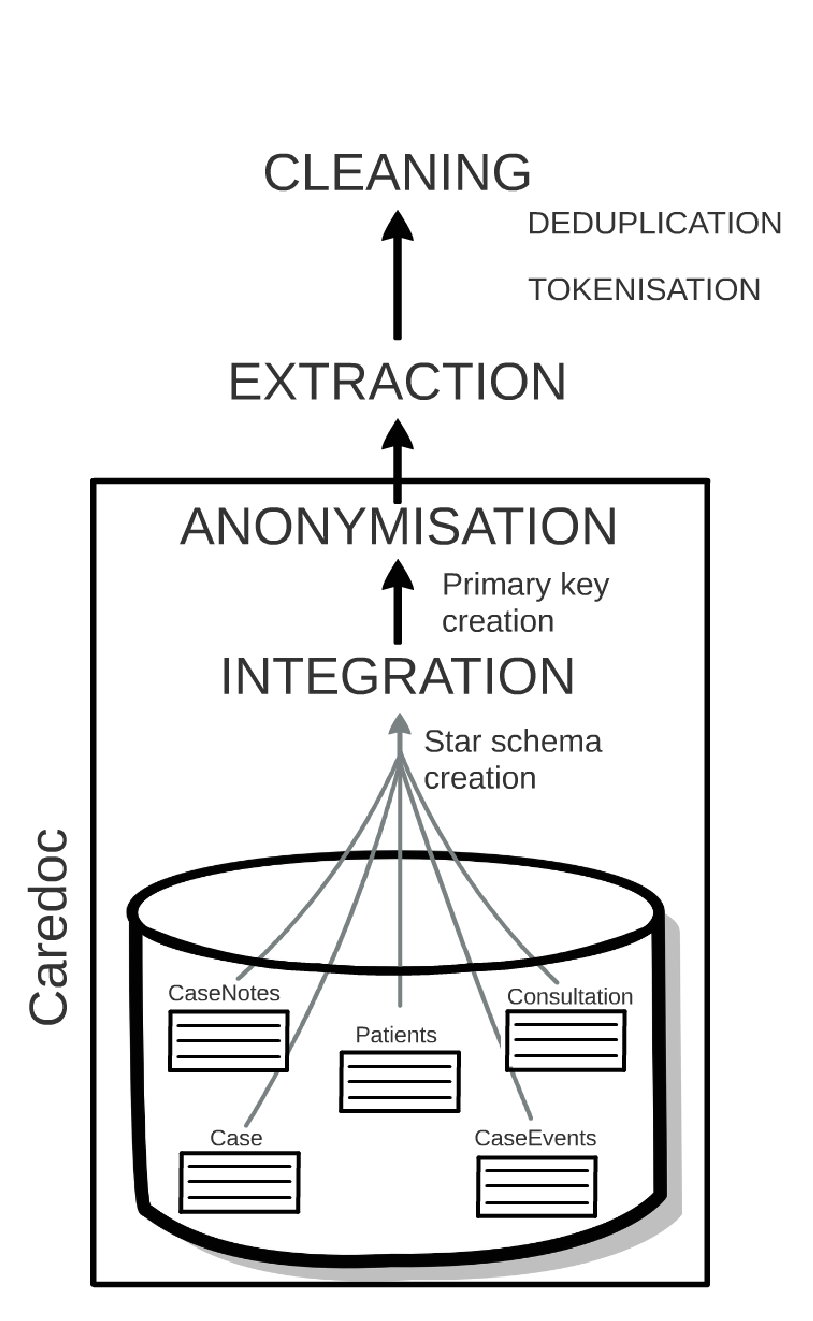
\includegraphics[page=1,width=0.7\textwidth]{data-flow3.pdf} & 
   \end{tabular}
  \caption{\hl{Data selection and extraction processes} used in relation to associate operational systems.}
 \label{fig:data-mining}
\end{figure}


The first step in this process involved collaboration with the domain experts of Caredoc\index{Caredoc} and identification of broad research goals, the latter of which have since formed the basis for this thesis. Once ethical approval for this research had been achieved, a series of goals were developed, as can be seen in Figure \ref{fig:data-mining}, that would be necessary for our use of this data. Removing historical data to a location where it could be subject to analysis without jeopardising systems that are in active use in a live medicinal setting was a research prerequisite. In order to achieve this an iterative set of queries which could extract data from the various sources under Caredoc\index{Caredoc}'s supervision had to be developed. This integration of data, from numerous independent tables, was primarily achieved using the pseudo foreign keys that were in operation in the Caredoc\index{Caredoc} systems.\footnote{An example of the internal Caredoc\index{Caredoc} data systems can be seen in Figure \ref{fig:internal-caredoc} in the appendices. Note that many of the attributes and tables in Caredoc\index{Caredoc}'s systems are not operable for multiple reasons, such as some of the tables being inherited from similar systems from the NHS and not being applicable in an Irish setting.} A single table which would form the corpus for our research was formed from the extracted information from the Caredoc\index{Caredoc} systems using the star schema \cite{han2011data}. As this was being created, a primary key for patients had to be simultaneously generated in order to help bind this data in a normalised manner. This key was produced using SHA-256 hashing \cite{rachmawati2018comparative} over a combination of patient name and date of birth. Patient personal details (such as name, day and month of birth, phone number, and address) were excluded from the process of data integration, ensuring that the corpus that was ultimately extracted from Caredoc\index{Caredoc}'s systems would contain anonymised patient details. 

In Figure \ref{fig:data-mining}, \textit{CaseNotes} is a linking table that contains a unique hexadecimal to reference other tables. \textit{Case} is the main table that contains information relating to a specific case for a patient. \textit{Consultation} is the main table that contains consultation information relating to a case for a specific patient. \textit{CaseEvents} contains information relating to a specific case and the time line for what happened to the case. \textit{Patients} contains the information relating to a patient who may have multiple cases attached to them. The extraction process flattened all of this information into a single table, from which all the research in this thesis is predicated. The rest of this chapter will give a high level analysis of this data, and the significance it may pose to this research.

Because the Caredoc\index{Caredoc} databases were non-normalised, duplicate case data could be created during normal operation of the OOHC\index{Out-of-hours Health Care}, and consequently made up part of the corpus that was extracted from Caredoc\index{Caredoc}. Absolute duplicate cases and empty cases were both straightforward to eliminate from the repository. However, staff at Caredoc\index{Caredoc} when dealing with patients occasionally copied case data and edited this copied data, instead of editing the original case entry. We accordingly developed an algorithm to search for exact strings in cases with identical case numbers, and deleted the original case data that had been copied by the phone operator. This reduced the final corpus from 310549 to 294337 cases.    

  \begin{figure}[ht]
   \centering
   \begin{tabular}{@{}c@{\hspace{.2cm}}c@{}}
 \includegraphics[page=1,width=1.20\textwidth]{graph-origin.pdf} & 
   \end{tabular}
  \caption{The collated dataset contained information obtained from a wide range of sources.}
 \label{fig:info-origins}
\end{figure}



%Extracting features from non-annotated, unstructured text creates distinct challenges. Clinical text is a patois designed to be human interpretable by persons with health care backgrounds who can infer meaning from context. The manner in which information is recorded is not only inconsistent from person to person, but moreover, is dirty: typically exhibiting spelling mistakes, shorthand, colloquial phrases, and truncated grammar. Although best practise guides exist which describe ways in which medical terms should be recorded by healthcare professionals, e.g. \cite{abbreviations}, there is no standard for the industry as a whole and adoption by individuals may be discretionary. Typically, as is the case in the dataset under investigation, medications, signs, and diseases can be written using a multitude of variants. The terse writing style and abbreviation of many words consequently restricts the number of Natural Language Processing (NLP) approaches which would be suitable to use upon the corpus \cite{tsujii2011computational}. Entirely ignoring syntactic context in favour of lexeme specific approaches (e.g. Bag-of-Word variants)\cite{zhang2010understanding} would not necessarily be appropriate. Not only is context important in developing robust means of cleaning the data, but the environment within which lexemes appear may have a substantial bearing on their importance (for instance, contextual negation) \cite{elkin2005controlled}.




%While this factor relating to the data in question is to some degree a technical deficiency owing to the manner in which telemedicine works in this particular environment, even were an exhaustive medical history of the patient available to the call-handler, its practical value would be diminished by the necessity for call-handlers to promptly handle and conclude calls. Manually parsing large volumes of medical information relating to the patient in question would hamper the performance of a triage. From the point of view of any algorithm that is developed within the scope of our research, the potential features available are inherently limited by the incomplete medical histories that are recorded about patients.       

\subsection{Description of dataset}
\label{section:dataset-description}





The aim of this section is to provide an overview of the key attributes of the dataset. Although some of the parametric data looked promising for predictive analysis, the inconsistent use and overly generic nature of these features by call operators told against their overall importance, as shall be explored below.

Very little parametric data was supplied in relation to patients themselves. While this was partially due to the anonymisation processes undertaken during data extraction, the patient parameters which were absent from this research, such as patients' addresses or phone numbers, would have likely provided meagre value from an analysis perspective. Personal medical data like patient height, weight, blood type, etc. were not collected by Caredoc\index{Caredoc} owing to the way in which OOHC\index{Out-of-hours Health Care} platforms function.     
 
% IN DEPTH DESCRIPTION OF DATASET
 
 %WHAT MAKES AN AVERAGE PATIENT
 
 %WHAT MAKES A FREQUENT USER?
 
 %EXPERT SYSTEMS should go into chapter 2.





 \begin{comment}
 \begin{table}[htbp]
 \caption{Description of numerical based information in extracted corpus}
\begin{center}
\begin{tabular}{|l|l|l|l|l|}
\hline
 &  mean & stdv &  min &  max  \\ \hline

dob &  1980.646 &  27.424 &  1900 &  2020  \\ \hline

month &  6.591 &  3.56 &  1.00 &  12  \\ \hline

day &  15.987 &  8.836 &  1.00 &  31 \\ \hline

cases &  6.35 &  23.629 &  1.00 &  395 \\ \hline

weekday &  3.929 &  2.399 &  1.00 &  7  \\ \hline

hour &  15.217 &  5.478 &  1.00 &  23 \\ \hline

minute  & 28.682 &  17.258 &  0.00 &  59 \\ \hline

second &  29.416 &  17.296 &  0.00 &  59 \\ \hline

case-no &  58554.323 &  23856.083 &  10001 &  99999 \\ \hline

Cons\_Time\_Taken  & 8.08 &  8.709  & 0.00 &  356 \\ \hline

\hline  
 \end{tabular}
 \end{center}

\end{table}
\end{comment}



 \begin{table}[htbp]
 \setlength{\tabcolsep}{8pt}
   \ra{1.2}
 \caption{Description of numerical based information in extracted corpus}
\centering
  \label{table:numerical-data}
\begin{tabular}{@{}c|cccc@{}}
\toprule
\multicolumn{1}{l|}{}      & \textbf{mean} & \textbf{std} & \textbf{min} & \textbf{max} \\ \midrule
\textit{dob}               & 1980.64       & 27.42        & 1900         & 2020         \\
\textit{month}             & 6.59          & 3.56         & 1.00         & 12           \\
\textit{day}               & 15.98         & 8.83         & 1.00         & 31           \\
\textit{cases}             & 6.35          & 23.62        & 1.00         & 395          \\
\textit{weekday}           & 3.92          & 2.39         & 1.00         & 7            \\
\textit{hour}              & 15.21         & 5.478        & 1.00         & 23           \\
\textit{minute}            & 28.68         & 17.25        & 0.00         & 59           \\
\textit{second}            & 29.41         & 17.29        & 0.00         & 59           \\
\textit{case-no}           & 58554.32      & 23856.08     & 10001        & 99999        \\
\textit{Cons\_Time\_Taken} & 8.08          & 8.7          & 0.00         & 356          \\ \bottomrule
\end{tabular}
\end{table}

Table \ref{table:numerical-data} describes the data contained within numerical (or predominantly numerical) fields within the corpus. Date of birth (DOB) was partially anonymised such that only year of birth was available, while month, day, weekday, hour, minute, second were generated from a single timestamp field. DOB on very rare occasions had textual information input such as `not stated' or `unsure'. These fields were replaced with the year 2020 for our purposes. This was done so as not to interfere with any numerical calculations made using this field throughout our research, whilst also clearly indicating the simulated nature of this data. Cons-Time-Taken generally related to how long specific phone calls lasted, though this field could also, on occasion, account for time taken in home visits. This value is measured in minutes. \hl{Occasionally Caredoc staff may fail to correctly record the time taken in the consultation, which will result in the value for this field being recorded as zero.}  
 
   \begin{landscape}
   \begin{figure*}[]
   
      \centering
      \framebox{\parbox{2.5in}{
}
      \includegraphics[page=1,width=1.8\textwidth]{graph-change.pdf}
      }
      \caption{Priority assigned to patient cases.}
      \label{fig:caller-priority}
   \end{figure*}
\end{landscape} 
 
 \begin{landscape}
   \begin{figure*}[]
   
      \centering
      \framebox{\parbox{2.5in}{
}
      \includegraphics[page=1,width=1.8\textwidth]{graph-caller+.pdf}
      }
      \caption{EHR parameter relating to patient relationship to caller, showing
high dimensionality and large volume of null values.}
      \label{fig:caller-relationship}
   \end{figure*}
\end{landscape} 


 
 \begin{figure}[]
   \centering
   \begin{tabular}{@{}c@{\hspace{.1cm}}c@{}}
 \includegraphics[page=1,width=1.00\textwidth]{dob-fas.pdf} & 
   \end{tabular}
  \caption{EHR\index{Electronic Health Record} parameter relating to patient date of birth.}
 \label{fig:caller-age}
\end{figure}

      \begin{figure}[ht]
   \centering
   \begin{tabular}{@{}c@{\hspace{.2cm}}c@{}}
 \includegraphics[page=1,width=0.60\textwidth]{graph-sex2.pdf} & 
   \end{tabular}
  \caption{Sex ratio of cases.}
 \label{fig:caller-sex}
\end{figure}




   \begin{figure}[ht]
   \centering
   \begin{tabular}{@{}c@{\hspace{.2cm}}c@{}}
 \includegraphics[page=1,width=0.80\textwidth]{Figs/graph-medical-card2.pdf} & 
   \end{tabular}
  \caption{Medical card status of patients.}
 \label{fig:caller-card}
\end{figure}
 
   There were some interesting non-numerical attributes relating to cases available within this research. This included the priority assigned to cases by call-operators (Figure \ref{fig:caller-priority}). The assigned priority could be changed (sometimes radically) after nurse triage, but typically this value wasn't altered. The vast majority of cases were classified as `less urgent'  The only other common classification was that of `urgent', but almost  half of these cases were downgraded to `less urgent' after assessment. The description of `less urgent ', and even to a lesser extent, ` urgent' are both very broad, and their consequent vagueness undercuts their capacity to provide insight into cases. For instance, these descriptions provide no indicator whether the cases in question relate to chronic or acute conditions. It is also unclear what precipitated the change of status of some of these cases from their initial handling by call centre staff, to nurse triage. 
%    \begin{figure}[h]
%   \centering
%   \begin{tabular}{@{}c@{\hspace{.2cm}}c@{}}
% \includegraphics[page=1,width=1.20\textwidth]{graph-change.pdf} & 
%   \end{tabular}
%  \caption{Priority assigned to patient cases.}
% \label{fig:caller-priority}
%\end{figure}
 
 
 
 
% \begin{figure}[]
%   \centering
%   \begin{tabular}{@{}c@{\hspace{.2cm}}c@{}}
% \includegraphics[page=1,width=1.20\textwidth]{graph-caller+.pdf} & 
%   \end{tabular}
%  \caption{EHR\index{Electronic Health Record} parameter relating to patient relationship to caller, showing high dimensionality and large volume of null values.}
% \label{fig:caller-relationship}
%\end{figure}
 
 

 
 Another interesting feature is that which describes the patient's `relationship to caller' - that is to say, the patient's relationship to the person who has actually called Caredoc\index{Caredoc}. Unfortunately this attribute was mostly filled with nulls. Where a value was recorded, the term `mum' was disproportionately represented. Values were otherwise sparse, as can be seen in Figure \ref{fig:caller-relationship}. It is difficult to determine, after the fact, whether this attribute was reliably populated by Caredoc\index{Caredoc} staff. For instance, it is not known whether a lack of information relating to this attribute consistently means that the patient themselves was the caller.
 

 
 Date of patient birth (binned by decade) can be seen in Figure \ref{fig:caller-age}. The small number of cases with no \hl{recorded date of birth (demarcated by `2020') is visible here (though it is possible that patients with a date of birth recorded as `1900' are also erroneous). While there a a large number of very young children (under the age of 4) treated as part of the total volume of cases, these still account for only 19\% of the total.}   
 

 
As may be apparent, demographic data was very limited, with most parameterised information being metadata relating to the call itself. The only demographic data recorded by Caredoc\index{Caredoc} related to the age, sex, medical card status, and address of the patients (the latter of which was not provided by Caredoc\index{Caredoc} in data related to this research). Parametric information detailing the sex of the patient can be seen in Figure \ref{fig:caller-sex}, and detailing the medical card status can be seen in Figure \ref{fig:caller-card}.  These features both had a small set of values, with little  noise.  
 

 
 Initial attempts to classify patients as either frequent or non-frequent users was performed using \hl{ the attributes discussed above} using Random Forest, linear SVM, and multivariate linear regression, as can be seen in Chapter \ref{chpt:machine-learning}.  
 

 
 
 
 \subsection{Free-text data}
 \label{section:free-text-description}
 
 \begin{table}[ht]
\setlength{\tabcolsep}{8pt}
   \ra{1.2}

\centering
\caption{Free-text data in corpus.}
\label{table:corpus}
\begin{tabular}{@{}lcccc@{}}
\toprule
\textbf{attribute} & \textbf{entries} & $\mathbf{\bar{c}}$ & $\mathbf{\bar{w}}$ &$\mathbf{\sigma w}$ \\ \midrule
olc\_history       & 15226            & 182.72                       & 16.58 & 23.4                      \\
olc\_examination   & 11326            & 115                          & 7.24  &11.9                      \\
olc\_diagnosis     & 120433           & 25.46                        & 1.66  & 3.65                      \\
olc\_treatment     & 123517           & 74.86                        & 5.61      &9.38                  \\
teleguides         & 58906            & 271.28                       & 38.95     &20.05                     \\ \bottomrule
\end{tabular}
\end{table}
 
 The vast majority of information relating to cases was recorded in the free text fields (of which there were four attributes, as can be seen in Table \ref{table:corpus}, where average count of word (w) and characters (c) is described, along with the standard deviation of word count $\mathbf{\sigma}w$). The `olc\_' delineation is a naming convention within Caredoc's relational database management system which indicates the presence of FTN.\index{free-text} The `teleguides' field has a slightly different use case, where it relates to free text notes concerning the use of the Nightingale system (described in Section \ref{Out-Of-Hours_Health-Care}). teleguides notes did not coexist with notes relating to any of the other four FTN fields. 
 These fields (the names of which in Table \ref{table:corpus} are taken directly from the Caredoc databases) were not consistently filled for each case treated, and the actual population of these separate fields only loosely corresponded to their purported purposes (of history, examination, diagnosis, or treatment of patients respectively). When more than one of these fields was filled, their usage was however consistently recorded in this temporal order. Consequently, if simultaneously present for a given case, these data were appended together when creating datasets for our classifiers.
 
 \newcommand*{\thead}[1]{\multicolumn{1}{c}{\bfseries #1}}
\begin{comment}
\begin{table}[h]
   \ra{1.3}
\caption{Free-text data in corpus}
\begin{center}
\begin{tabular}{|l|l|l|l|}
\hline
\textbf{attribute}     & \textbf{entries} & $\mathbf{\vert\bar{c}\vert}$ & $\mathbf{\vert\bar{w}\vert}$   \\
\hline
olc\_history   & 15226  & 182.72 & 16.58 \\

olc\_examination & 11326  & 115 & 7.24 \\

olc\_diagnosis & 120433  & 25.46  & 1.66  \\

olc\_treatment    & 123517  & 74.86  & 5.61 \\

teleguides & 58906 & 271.28 & 38.95 \\
\hline
\end{tabular}
\end{center}
\label{table:free-text}
\end{table}
\end{comment}

 % Please add the following required packages to your document preamble:
% \usepackage{booktabs}

 


 Decision support systems based upon predicative analysis have had limited application in real world environments. One of the reasons for this is that EHR\index{Electronic Health Record} data is challenging to represent and model due to its high dimensionality, noise, heterogeneity, sparseness, incompleteness, random errors, and systematic biases \cite{botsis2010secondary}. While a wide range of parametric data was contained within the data provided, early testing showed that these fields alone were insufficient to build successful models from. We thus looked to the FTN data to provide the cornerstone of predictive analysis. The following chapter will detail measures we took to improve the features of this textual data.

The untreated corpus free-text\index{free-text} featured 131841 unique lexemes, and a linguistic diversity of 0.072 where linguistic diversity, \textit{d}, is defined as the set of terms \{\textit{t}\}, over the frequency of terms |\textit{t}| in the dataset.

\begin{comment}
\begin{align}
d: \hspace*{5mm}\left \|\frac{\left\{t\right\}}{\left \| t \right \|}  \right \|
\end{align}
\end{comment}

\begin{align}
d: \hspace*{5mm}\left |\frac{\{t\}}{|  t | }  \right |
\end{align}




 \subsection{Frequent User Data Characteristics }
 
 Frequent users are an \hl{unusual}, but significant subset of patients in our dataset. The distribution of cases relative to frequency of interaction can be seen in Figure \ref{fig:graph:cases}, showing that the vast majority of interactions with the OOHC\index{Out-of-hours Health Care} are ``non-frequent". 
 
 A balance in relation to clinical application was a significant priority; where a threshold should be adopted that would clearly establish a given patient as meriting investigation, but would not apply unnecessarily restrictive parameters on the definition of the cohort.  While the definition of frequent user based upon some temporal category was considered, this was dismissed due to a number of considerations. First, as the dataset was exclusively collected over the period of a single calendar year, there was already an implicit temporal demarcation. Second, the main concern relating to frequent users was that of persistent, unresolved medical issues, which unusually high contact over a short period of time (for instance, over the period of a couple of weeks) would not represent.
 
A working figure of 40 cases was initially established in the research as the threshold that patients were determined to be frequent users. This was later revised down to 24 cases in order to capture a larger cohort. 
 
 
A final potential means of defining frequent users lay in the absolute amount of time that patients interacted with Caredoc. This approach would deviate significantly from the way in which frequent users are typically defined \cite{holmstrom2017frequent}, but could in theory be used by specifying a certain percentile for summed consultation times over all cases for each patient. For our purposes, the mixed nature of data (relating to calls, treatment centres, and home visits), the potential for incorrect or missing data relating to the calculated duration of cases, and the fact that a threshold based upon time would be an inferior metric (compared to cases as a means of determining the frequency of interaction between patients and the OOHC in question), all told against consultation time as a means of defining a threshold.  
 
 

 
 
 Ultimately a third category of high frequent user, similar to that pursued by Bhroin et al.\cite{bhroin2019profiling}  was used to describe patients with more than what was roughly twice the baseline rate. This threshold was left at the discretion of Caredoc for potential future application on their part, as the threshold figure could easily be revised either up or down, as demanded by the organisation.  
 
 For this thesis, unless otherwise stated, frequent users will be defined as patients who had at least 24 interactions with the OOHC\index{Out-of-hours Health Care} for the calendar year of 2014. 
 
 
 
     \begin{figure}[thpb]
      \centering

      \includegraphics[scale=0.36]{graph-case-frequency.pdf}

      \caption{Case:frequency distribution}
      \label{fig:graph:cases}
   \end{figure}
   
   
As can be seen in the description of the meta data related to frequent user cases in Table \ref{table:frequent-users}, the cohort representing frequent users have a relatively similar general profile to most other users. The average age relating to frequent user cases is somewhat \hl{higher} (with a birth year mean of 1960 as opposed to 1980 for the corpus as a whole) and there's a higher prevalence of medical card holders (88\% as opposed to 67\% for the corpus as a whole). However other features do not immediately jump out as being particularly discriminative. Sex ratio and consultation times are very similar to the rest of the corpus. Priority on reception, measured from 1 (not urgent) to 4 (palliative) shows that, like the rest of the corpus, most cases belonging to this cohort were classified as `non-urgent'. \hl{Though the consultation time taken is on average slightly lower than for patients in general (7 minutes as opposed to 8 minutes), it is not statistically significant. Indeed the difference in the mean is an order of magnitude smaller than the standard deviation in this regard.}       
   
   
   
% Please add the following required packages to your document preamble:
% \usepackage{booktabs}
\begin{comment}
\begin{table}[h]
\begin{center}
\begin{tabular}{@{}l|l|l|l|l|@{}}
\cmidrule(l){2-5}
                                        & \textbf{mean} & \textbf{std} & \textbf{min} & \textbf{max} \\ \midrule
\multicolumn{1}{|l|}{dob}           & 1960.944 & 22.362 & 1919 & 2020 \\ \midrule
\multicolumn{1}{|l|}{male}          & 0.438018 & 0.4962 & 0    & 1    \\ \midrule
\multicolumn{1}{|l|}{medical\_card} & 0.886897 & 0.3167  & 0    & 1    \\ \midrule
\multicolumn{1}{|l|}{weekday}       & 3.939715 & 2.3422 & 1    & 7    \\ \midrule
\multicolumn{1}{|l|}{hour}          & 14.87261 & 6.8705 & 0    & 23    \\ \midrule
\multicolumn{1}{|l|}{priorityonreception} &	1.352342 &	0.5878 &	1 &	4 \\ \midrule

Cons\_Time\_Taken & 7.098167 & 8.4696 & 0 & 185    \\ \bottomrule
\end{tabular}
\end{center}
\end{table}
\end{comment}

% Please add the following required packages to your document preamble:
% \usepackage{booktabs}
% Please add the following required packages to your document preamble:
% \usepackage{booktabs}
\begin{table}[h]
\setlength{\tabcolsep}{8pt}
   \ra{1.2}
\centering
\caption{Description of frequent user meta-data.}
\label{table:frequent-users}
\begin{tabular}{@{}c|cccc@{}}
\toprule
\multicolumn{1}{l|}{}        & \textbf{mean} & \textbf{stdv} & \textbf{min} & \textbf{max} \\ \midrule
\textit{dob}                 & 1960.94      & 22.36        & 1919         & 2020         \\
\textit{male}                & 0.43      & 0.49        & 0            & 1            \\
\textit{medical\_card}       & 0.88      & 0.31        & 0            & 1            \\
\textit{weekday}             & 3.94      & 2.34        & 1            & 7            \\
\textit{hour}                & 14.87      & 6.87        & 0            & 23           \\
\textit{priorityonreception} & 1.35      & 0.58        & 1            & 4            \\
\textit{Cons\_Time\_Taken}   & 7.09      & 8.47        & 0            & 185          \\ \bottomrule
\end{tabular}
\end{table}




Frequent user case FTN had a general lower linguistic diversity from the rest of the corpus (0.058 to 0.072 respectively). In Chapter \ref{chpt:machine-learning} we will examine the viability of FTN, relative to parametric data, to potentially classify these cases.  


\section{Summary}

Frequent users are a complicated subset of patients. Unlike typical disease prediction, frequent usage is not in itself a specific illness, but is rather indicative of certain morbidities that are not being resolved through available primary or secondary care. Targeting frequent users with public health initiatives appears to be a priority, but the development of means to accurately predict frequent users is a complicated problem. This largely stems from the diverse characteristics of frequent users, paucity of available data, and the quality and precision of data that is available.  

Limitations concerning information relating to patients (both frequent and non-frequent users) generally stems from the restricted nature of the dataset being examined (both institutionally and temporally). As discussed earlier in this chapter, this research must be conducted without any knowledge of patient interactions with healthcare outside of Caredoc\index{Caredoc}'s auspices, nor can it consider interactions outside of 2014. However, as demonstrated with recourse to relevant literature, there is significant evidence to show both strong correlations between high use of different levels of healthcare, and the non-transitory nature of frequent user healthcare needs.

This section detailed how we created the corpus that was used throughout this research, and overcame some of the structural shortcoming the databases in our industry partner suffered from. A general description of the data was provided in this chapter, from which it is clear that significant volumes of data exist to describe cases. Nevertheless it is not obvious \textit{a priori} which features may prove most important in the classification task. 

 \chapter{Related Research}
\label{chpt:related-research} 


 

 
 
\section{Introduction}

In this section the literature relevant to this thesis in both prediction of patients, and treatment of textual features related to patient cases is reviewed. In addition, a survey of the different objectives that are the most recurrent is presented. Given the volume of the literature, only the most significant works amongst them are presented. Much of the literature in this chapter will relate specifically to the problem domain, while additional literature relating to potential solution implementations will be addressed in \\ Chapter \ref{chpt:machine-learning}.

\section{Patient Classification}



\subsection{High Use Prediction}

There is no extant work predicting high use patients of non emergency OOHC\index{Out-of-hours Health Care}. To the extent there is research concerning frequent users in other settings, prediction is at most limited to regression analysis, typically of well structured data that requires minimal processing. While many researchers agree that early detection of frequent users is an important area of research \cite{vu2015screening,chan2018frequent,meng2017disordered}, the exact characteristics that represent frequent users is an area that is currently not well understood.    
Logistic regression using standardised information derived from EHR\index{Electronic Health Record} is the predominant means by which FA use of ED has been achieved to date \cite{billings2013dispelling,smits2013predictability,scott2014describing}. However there are some characteristics which distinguish the leading researchers in this area. 

Smits et al. have worked extensively on the analysis and prediction of frequent attenders in general practice using clinical data obtained in the Netherlands \cite{smits2009predictability}. Each patient analysed by Smits et al. has had an associated list of current medical problems, known as a \textit{problem list}. These problem lists are compiled by the patients' GPs, and describe any medical problem (disease or complaint) which needs continuing medical attention or monitoring. They also detail  any complaint or disease present for more than 6 months (excluding all (minor) short episodes) \cite{smits2009predictability}. Each problem on each list was coded using the International Classification of Primary Care  \cite{bentsen1986international,verbeke2006international}. Having more than one year's worth of data, Smits et al. were able to distinguish between frequent attenders and persistent frequent attenders (that is to say, FAs that remained FAs for multiple years) \cite{smits2013predictability}. 


While it is possible that these problem lists featured overreported problems (complaints that were merely historical and had already been resolved), and may not contain some psychological conditions \cite{smits2013predictability}, the type of dataset  that Smits et al. were typically considering was very clean, and thus in a state suitable for multivariable logistic regression analysis. Smits et al. achieved an area under the curve of the receiver operating characteristic \footnote{this metric will be discussed in more detail in Section \ref{section:LSTM-results}} of up to 0.67, which they show to be the effective ceiling to this approach in the absence of better predictors \cite{smits2013predictability}. This is therefore an example of well codified data that nonetheless had significant limitations in its capacity to identify the target group. Notably, the introduction of features representing the presence of medically unexplained problems, prescriptions of psychoactive drugs and antibiotics had provided no improvement in the capacity to predict frequent attender patients.   



%: The existing model (c-statistic 0.67) discriminated moderately with predicted values between 7.5 and 50 percent and c-statistics of 0.62 and 0.63, for validation in the original network and SMILE network, respectively. Calibration (0.99 originally) was better in SMILE than in the original network (slopes 0.84 and 0.65, respectively). Adding information on the three new predictors did not importantly improve the model (c-statistics 0.64 and 0.63, respectively). Performance of the model based on the combined data was similar (c-statistic 0.65).

%This model included the variables: age (Odds ratio (OR) 0.99 per year), number of active problems (OR 1.13 per additional problem), presence of any chronic somatic problems (OR 1.55), any psychological problems (OR 1.72) and the monthly number of analgesic prescriptions (.4: OR 2.06). [14] \cite{smits2013predictability}

%Five predictors were retained in the final model: age, the number of problems on the GP's problem list, presence of any of three chronic somatic illnesses (diabetes mellitus, cardiovascular illness, and respiratory illness), presence of a psychological/social problem, and the use of pain medication (Table 2). None of the interaction effects proved significant at the 10\% level. The prior probability of 15.4\% (470/3045) of persistent frequent attendance could be updated, using the model, to at best 3.3\% (lowest value) or 43.3\% (highest value). The 10th and 90th centiles of the posterior probability distribution were 7.4\% and 26.3\% respectively, indicating that the model does not perform very well either to rule out persistent frequent attendance or to rule it in. The Hosmer–Lemeshow test showed a P-value of 0.254, thus indicating no strong evidence against good model fit. As a summary of the model's overall discrimination, the model's area under the receiver operating characteristic curve (AUC ROC) was 0.67 (bootstrapped bias-corrected 95\% CI 0.64 to 0.69).
%\cite{smits2009predictability} % ^^^ SAME GUY!

As stated above, research concerning frequent callers is much thinner on the ground than that concerning frequent attendance. This makes prediction involving FC (specifically relating to ambulance services in this case) as performed by Scott et al.\cite{scott2014describing} exceptionally rare. This research, like that discussed above, again presents the usage of multiple regression analysis, albeit including some metadata specific to calls such as ‘date of call’ and  ‘time of call’. However, Scott et al.'s research was not designed to predict patients \textit{per se}, but rather as an explorative measure to identify what circumstances are most associated with a patient being an FC. Similar to Smits et al.'s research, the primary feature used was a dispatch code, which despite \hl{being} a different type of encoding from that featured in Smits et al.'s work, was nonetheless a standardised code that boasts a large usage basis within the medical domain. However only 74.5\% of call data had valid dispatch numbers. Scott et al. discovered a strong correlation between dispatch codes relating to `sick person' and `psychiatric' behaviour, while codes relating to falls and those from a `Healthcare professional' were inversely related to FC.


%For the top 100 frequent callers, the \b{Shapiro–Wilk} test indicated that the total calls (p<0.001), number of different reasons for calling (p=0.016) and number of times conveyed (p<0.001) were not normally distributed, but the age of the callers (p=0.357) was normally distributed. Multiple regression analysis was conducted to determine which primary call reasons were able to predict the total number of calls made by the top 100 frequent callers. The assumptions of linearity, normality, reliability and \b{homoscedasticity} were not met,16 so the data was cleaned. A \b{Cook's Distance} (Di) value of >1 was used to remove patients (n=4, Di=1.281 to 2.841) with a large influence on the data. Once these outliers were removed, \b{variance inflation factors} (VIFs) of >10 were used to determine any collinearity (n=0). A plot of the \b{studentised} residuals was then used to remove any outliers (n=4), identified by being >3 SDs away from the mean. The \b{Breusch–Pagan test} was then used to determine homoscedasticity (x2=0.00015, df=1, p=0.990) and VIFs ranged 1.075–3.612. The final multiple regression analysis contained 92 participants. \cite{scott2014describing}


%(Mostly `sick person' and psychological issue indicated frequent caller, while healthcare professional call and falls indicated a non frequent caller.)
%Significant predictors are shown in Table 1. ‘breathing problems’ and ‘sick person’ contributed the most to the model, followed by ‘psychiatric/abnormal behaviour/suicide attempt’, ‘abdominal pain/problems’, ‘chest pain’ and ‘falls’. For most call reasons, for one call increase in the independent variable, there was approximately one overall call increase. The two main exceptions to this were ‘choking’ and ‘assault/sexual assault’, which increased by 4.5 Calls for codes ‘healthcare professional call’ (95\% CI 0.402 to 2.885) and ‘sick person’ (95\% CI 1.398 to 1.694) resulted in around 1.5 more calls overall.\cite{scott2014describing}

Pasgaard et al.'s research featured a very extensive survey which was used to establish the socio-demographic status of some 23384 individuals (supplemented with information from the Income Statistics Register, Population Education Register, Danish National Health Service Register, and Danish Civil Registration Register) \cite{pasgaard2018social}. Like much other research into frequent users, cutoff values were used in the definition of frequent attendance. This sort of study conducted by Pasgarrd et al. looks at data concerning `social capital' \cite{coleman1988social} which medical analysis typically doesn't have access to \cite{frost2017using}. As such, while it produced some interesting insights into individuals' perceptions of their place in society, and the connection this may have with frequent attendance, it is difficult to see how one may ameliorate existing data sources which do not contain such in-depth user survey information. Prediction was performed using the Random Forest algorithm, but this work was performed merely to determine characteristics of frequent users, and no testing was performed to ascertain the accuracy of using extracted  frequent user characteristics on unseen data to determine which patients may be, or become, frequent users. 

Frost et al.'s prediction methodology \cite{frost2017using} is research which most closely relates to this thesis. Frost et al. produce a comprehensive prediction methodology in the context of FA utilising ED. Frost et al. unlike some of the researchers mentioned above, explicitly randomly split their data into training and validation cohorts (although no testing cohort is present). An unusual aspect of this research is that only patients over the age of fifty are considered, owing to particular motivations in relation to FA intervention on the part of Frost et al. To the best of the author's knowledge, this study marks the only known existing research to use free-text\index{free-text} in FA prediction. Lexical tokens were extracted by these researchers from patient case text, and filtering was performed to remove stop words and infrequent terms. This study had access to multiple years of data, so these researchers were able to use the data from one year to predict occurrences in the subsequent year. A slight peculiarity of this study is that it delineated patients both upon total number of visits, and also in terms of total costs associated with those patients. AUC ranged from 0.7 to 0784, depending on the type of prediction being made. Frost et al. point out the absence of any known extant prediction relating to high use of ED based upon primary care EHR\index{Electronic Health Record} data. 


%We dichotomized this variable into frequent attenders, who constituted the upper quartile of utilization (>.32 consultations over the 148 week period), and others. A number of different cutoff values are used in the literature in regards to operationalizing frequent attendance, the current approach was chosen on the basis of previous literature [10] and different cutoffs are tested to ensure the robustness of the operationalization.\cite{pasgaard2018social}

%The association between the four dimensions of social capital and frequent attendance within 148 weeks of follow-up was explored through logistic regression. The unadjusted odds ratio (model 1) was estimated for each of the four social capital dimensions in individual models. Model 2 included age, education and income as potential confounders. Model 3 included the same variables as model 2, with the addition of the physical and the mental health component scores of the SF12.\cite{pasgaard2018social}

%To minimize a potential bias due to missing values (Additional file 1), multivariate imputation by chained equation (MICE) [35] was used. MICE is generally the preferred method of imputation when missing values occur in several different types (i.e. categorical, continuous etc.) of variables in the data set [36]. The method used for prediction was Random Forest, a machine learning technique well suited to handle nonlinearities and high dimensional data [37, 38]. Nonlinearities were suspected due to the complex relationship between gender and social capital. The imputation model featured all variables included in analysis models, as well as several additional variables from the original dataset, to satisfy the “missing at random” assumption [36]. The R code used for the imputation and a list of variables used are available in Additional file 1.\cite{pasgaard2018social}

%All results are reported as odds ratio with an estimated 95\% confidence interval. The primary analysis was carried out on the imputed data, and the results reported are pooled according to Rubin’s rules [39].

Readmission prediction is an area obliquely related to the topic of this thesis and will not be considered as part of related literature. While nominatively both readmission and frequent users are similar in that they both relate to a patient repeatedly utilising medical services, most of the aspects of these respective fields of study are divergent. Readmission refers exclusively to secondary and tertiary health care, and generally relates to unanticipated follow-up care very shortly after a patient's treatment has concluded (usually within 30 days of such) \cite{brudvik2015definition}. Readmission may reflect badly upon the healthcare provider, and certain systems penalise hospitals which experience higher than anticipated rates of readmission \cite{fonarow2017hospital}. Furthermore, readmission research typically focuses on a specific medical subdomain, such as myocardial infarction \cite{kociol2012international}, stroke \cite{boehme2018infections}, transplant surgery \cite{covert2016predicting}, etc. Finally, owing to the origin of this data, case information derived from EHR\index{Electronic Health Record} for readmissions are likely to feature standardised recording methods.        


\subsection{Disease Prediction }

The task of identifying a set of patients for community based intervention, based upon certain characteristics common to this cohort, shares some conceptual ground with disease prediction. Disease prediction is an area of research renowned for its difficulty. Where a patient presents with clear signs, human physicians are typically considered the optimal means of  providing diagnoses. However, individuals may exhibit characteristics that indicate the propensity for a disease that are themselves relatively innocuous, at least in isolation. This is particularly the case when these characteristics may be shared among a large population \cite{vos2016global}. The presence of characteristics that may potentially be indicative of a disease, that place a strain on the capacity of human cognition to discern patterns, include when these characteristics have no known direct association with that disease in existing literature; where such characteristics are apparently too generic to be useful; or where there are non-obvious interactions between different characteristics. The greater the volume of data that is required to identify previously unknown patterns, the more substantial a burden this poses, from a human perspective. 

These aspects lend themselves to a machine learning approach to developing predictive models. However, the different approaches taken to disease prediction is dependent on the types of features available for classification purposes. 

If the features are highly correlated to the prediction problem, feature selection is not a significant issue. For instance in Singh et al.'s prediction system for heart disease \cite{singh2018effective}, the features available included the type of chest pain experienced by the patients, their fasting blood sugar, resting blood pressure, whether or not they experienced exercise induced angina, their serum cholesterol, whether or not the patients were obese, etc.

Many of the feature selection processes in medicine assume scalar or categorised data presented in a consistent or normalised form. Most of the feature selection techniques that can be employed on this medical data fall into filter and wrapper techniques, which despite information gain and accuracy, suffer from potential disadvantages related to the independent consideration of features, and poor performance in high dimensional data-sets, respectively \cite{long2015highly}.

Occurrence of specific diseases in large populations are, by their nature, aberrant. Disease prediction conducted among apparently healthy individuals must thus weigh the likelihood of disease occurrence against the importance of its detection. A system which is biased in favour of the majority class (that is to say, a lack of occurrence of a given disease) may have an exceptionally high accuracy without actually detecting any true positives. It is clearly not acceptable for a public health system to be right `most of the time' if it fails to adequately treat the population it is meant to service.        

\begin{comment}
****************************

Correlation based feature selection (CFS)
Variables Importance (VImp)
Recursive Feature Elimination (RFE)
hamming distance

post- hoc (model agnostic) explainability as opposed to ante-hoc (model specific) explainability is what you are doing. 


XAI (explainable AI)





Diseases are rare

Some disease prediction works well with parameterised data. Like height and weight, age, bloods, protein markers, medications

When it comes to narrative based histories things get a lot more difficult

Extract from these histories. What's wrong with that? Trying to account for unforeseen, or unseen types of data. Basically hard coded. Context can be important. Negex has been developed to this end.

Words like other words. Is bleeding like cut? Is hospital like emergency room? Is nurse like doctor?
\end{comment}

\subsection{Free Text Classification}

It is self evident that not all words have the same potential value in terms of classification, but this is arguably particularly the case in a medicinal context, where content may be particularly loaded. While NLP in general may treat common words, such as prepositions, to be so generic as to pose inconsequential value, hyponyms in the medical domain would be typically considered to bear more value due to their specificity (compare `disease' and `diabetes'). Similarly, terms which relate to more serious conditions may be considered more `weighty' than those relating to more minor ailments (compare `infarction' and `bunion'). The same discrimination could be made in relation to medications (for instance `acetylsalicylic acid' and `morphine'). Classification using FTN generally forms two different approaches: either the discarding of lexemes which are deemed less important, or the analysis of wholesale context and the bearing this poses on the overall meaning of the text.




%based upon 



\section{Medical Text Processing}
\label{section-rr-medical-text}

%HOW DOES THIS CONTRIBUTE TO ORIGINAL RESEARCH


%WHAT IS THE STUFF THAT YOU HAVE LOOKED AT THAT HAS NOT BEEN LOOKED AT BEFORE?

%DECENTRALIZED HEALTHCARE

Standardised recording of medical data may relate to pharmaceutical codes, procedural codes, diagnostic codes or topographical codes. Some EHR\index{Electronic Health Record}, particularly where EHR\index{Electronic Health Record} are used in the course of patient financial claims, may have structured or encoded fields relating to major coding standards such as the International Classification of Diseases (ICD) and Systematized Nomenclature of Medicine (SNOMED) \cite{kharrazi2018value}. While ICD-10 is habitually used in the Hospital In-Patient
Enquiry (HIPE) scheme in Ireland \cite{hipe2018}, for hospital inpatient attendances and is linked to financial reimbursement from paper based records, it is significantly underrepresented in primary healthcare. The use of such encoded fields produces significant administrative overhead \cite{goroll2017emerging}, and many systems, such as the one under investigation in the course of this thesis, use neither encoded fields nor standardised codes to refer to diseases or treatment. Instead, diseases and symptoms can take a plurality of forms, may be misspelled or abbreviated, or are simply vague. This makes ontological use with the free-text\index{free-text} notes problematic, and adds significant complexity to the task of extracting useful data from patient case records.

FTN in EHRs\index{Electronic Health Record} are written in natural language, and research concerning their usage exhibit some of the same challenges as witnessed in other processing in natural language conducted in other domains. These challenges, broadly speaking, are primarily concerned with noise and ambiguity. A great deal of literature has been produced in recent years in relation to data mining and machine learning in  the context of social media, which chiefly concerns text based natural language information posted by users. However, social media text, such as that found on Twitter or Facebook, is not entirely analogous to medical FTN. 

For one thing, social media posting covers a multitude of domains \cite{deng2017adapting,leiner2018functional}, and means to successfully categorise tweets or Facebook posts is itself a laborious process. FTN on the other hand are almost exclusively related to diseases, signs, symptoms, advice, and medications. A significant difference between the NLP of social media, and NLP relating to FTN is the intended audience of the respective text. Whereas social media is typically written for a wide audience, the natural language in FTN is written by medical professionals, exclusively for use by professionals within the medical domain, and comprehension of such notes by people unused to the register employed in this environment would be quite difficult \cite{friedman2002two}. Furthermore, the writing style employed in the composition of FTN is terse, and may omit verbs, determiners, and other parts of speech that are usually used as the syntactic glue for natural language \cite{bunkenborg2019implementing}. The fact that FTN are composed in a time sensitive environment is a significant contributor to this type of writing style. Finally, albeit a less important issue, is the fact that personal opinion is omitted in FTN, thereby diminishing the volume of sentiment, and the degree to which sentiment analysis can be employed, within the FTN. 

 Annotated text datasets are a useful tool in the context of NLP\index{Natural Language Processing} tasks. Particularly in the circumstance of domain specific text, manual labelling provides excellent recourse to developing extraction and interpretative techniques through rule based systems. However, such datasets must be created by hand by experts, necessitating large volumes of work \cite{dietrich2019replicating}. Besides the cost and time involved in curating such data, lack of adaptability (both from a temporal and context point of view) disfavours such an approach. 



As the FTN are composed of data relating to diseases, signs, symptoms, advice, and medications, it thus follows that DM techniques need to be developed to treat these salient features. 

\subsection{Terminology Extraction}
\label{section-rr-terminology-extraction}

In counterpoint to the issue concerning ambiguity of overloaded signifiers resulting in polysemy, terms that are legitimate, but have multiple polymorphs, are known to reduce the effectiveness of machine learning if each polymoph is extracted as a distinct feature. An additional issue is the way in which diseases are frequently recorded in acronymised form, and drugs referred to by specific product names (e.g. “disprin” instead of “aspirin” or "acetylsalicylic acid"). 

While lemmatization can provide a suitable option for simple words by resolving root forms, and for well recognised entities Named Entity Recognition (NER)\cite{nadeau2007survey} can successfully provide generalisation, the medical textual domain is somewhat unsuited to both these techniques.

Lexemes relating to diseases, drugs or symptoms rarely provide forms suitable to any sort of stemming exercise. The root forms of these features are often more conceptual than morphological: for instance “chronic obstructive pulmonary disease” should be abstracted as a “respiratory” disease. NER would also prove unsuitable to this type of domain word, albeit for a different reason. Even if it could be successfully applied, which would in itself be problematic, NER would typically remove disproportionate value were it to merely classify diseases, drugs, and symptoms as such. That is to say that while feature abstraction is a potentially useful pursuit \textit{per se}, it nonetheless clear that, for instance,  a level of abstraction whereby terms like `rash', `tonsilitis', `lupus', and `anorexia' were replaced by tokens merely denoting `disease', would represent the loss of a significant amount of valuable information.

Despite the dirty nature of free-text\index{free-text} and colloquial language often used, the domain specific nature means that many of the issues surrounding the investigation of other media for medical related phenomena (such as those experienced by Paul et al. when treating Twitter data for disease related terms)\cite{paul2012model} are circumvented.

%ADD SOME NLP MEDICAL PAPERS HERE

\subsection{Medication Identification}
\label{section-rr-medication-identification}

Much of the relatively recent interest in medication extraction was precipitated by the i2b2 competition of 2010 \cite{demner2018finding}, which generated a substantial amount of literature on the topic over a relatively short period.  

The same general problems repeatedly arise when approaching clinical notes: the presence of both semi-structured and unstructured textual data (the latter of which contains high value domain terms), the relationship these terms have upon each other in free-text\index{free-text} environments, and the means by which this data can be transformed in order to provide meaningful analysis. To date, medications have predominantly been discovered in text through use of comprehensive predefined lists, though some work may be done to overcome the shortcomings of such an approach. 

Conventional wisdom states that even the most sophisticated algorithms cannot overcome all the limitations of poorly collected medication history at the point-of-care, such as open-ended free text fields, non-standard abbreviations, or invalid combinations due to uncontrolled data capture \cite{bennett2012utilizing}. Instead, ideally speaking, medication names should be correct at the time of their recording, and be in accordance with data standards \cite{richesson2010achieving}.

 
RxNorm\index{RxNorm} is an ontology based upon the Unified Medical Language System (UMLS)\cite{bodenreider2004unified} that is related to medication, and designed specifically to record all medications available in the United States of America \cite{nelson2011normalized}. Where medication names are well recorded, this ontology may be used to extract medications from medical text. This works well with suitably written medical text, such as publications found in the PubMed \index{PubMed} database \cite{kanavos2014pubmed}. Of course this necessitates that drugs (and potentially other medications) are recorded in a manner that matches that of RxNorm\index{RxNorm}. 

Using a predefined ontological list is a relatively simple but naive approach to extract medications. Nonetheless it has worked well for numerous researches, depending on the particular dataset. For instance  Levin et al. looked at the issue of discovering drug names in free text relating to preoperative drug history contained within anaesthesiologist EHRs\index{Electronic Health Record} and used the list approach, based upon RxNorm\index{RxNorm}, extensively  to this end \cite{levin2007extraction}. While a variant of the Soundex algorithm \cite{mckenna1998client} was employed in the course of this research to increase recall of pharmaceuticals, their strong results show that in certain circumstances ontological approaches can be successful \cite{levin2007extraction}.


%This , with a variant of Soundex applied in order to increase recall of pharmaceuticals. This approach seems partially inspired by the overarching design to match proprietary names to generic equivalents. Ultimately, Levin et al. achieve an exceptionally high PPV (Positive predictive value) of 98.8\% but a decidedly more modest NPV (Negative Predictive Value) of 76.2\%. 

Hua Xu et al. also based their system largely off of RxNorm\index{RxNorm}, and supplemented their findings using a regular expression tagger \cite{xu2010medex}. Filtering of English words in this system is based upon the Spell Checker Oriented Word Lists (SCOWL)\index{Spell Checker Oriented Word Lists} repository \cite{atkinson2004spell}. The system that Hua Xu et al. employ required some degree of manual inspection of ambiguous terms to be conducted by a physician, but seems to have had some capacity to handle abbreviations that were hitherto unknown by the system. However, the exact means by which abbreviations are mapped to their longer forms is not explored.  Results comparable with Levin et al.'s paper were achieved with an F-measure of 92\% on clinical notes. 

Yan Xu et al. were among those who used the 2010 i2b2 dataset to further investigation into the processing of medicinal textual data \cite{xu2012named}. Unlike some other research, the annotations supplied with the dataset were used solely for testing purposes by Yan Xu et al. As such, one of the primary ambitions of the research lay on the successful extraction of medical concepts within the free text notes of the i2b2 dataset. 

Although the i2b2 2010 challenge established the named-entities of ``medical", ``problem", ``treatment", and ``test", Yan Xu et al. identified that members of these classes did not necessarily appear in a similar manner to one another. In particular, Yan Xu et al. established a sub-class of "treatment" relating to medication, due to the fixed distinct semantic pattern that pharmaceuticals tended to take within the corpus. Consequently, an elaborate regular expression solution was built to capture these particular concepts.    

Attempts to define medications purely through use of a predefined ontology (namely UMLS) fared poorly for Yan Xu et al. due to the abundance of lexical variations that medications were subject to. Due to the variety of trade names and synonyms, Yan Xu et al. declared that it may be ``impossible'' to construct a dictionary that will reflect this plurality yet reliably stay up-to-date. 

Yan Xu et al. attempted to deal with the ambiguity of acronyms and abbreviations by using clustering of both types of contraction into their respective classes (i.e. ``medical'', ``problem", ``treatment", and ``test"). This clustering was based upon the distributional and morphological information of the lexemes. This is, however, confusing, as the means of discovering such lexemes is not described, and acronyms and abbreviations by their nature tend to offer poor morphological information.  

While clear that rule based systems are a crucial part of the solution provided, Yan Xu et al. elaborate that the output of the rule based systems was not an end product in itself. Rather, the output from these rules was fed to classifiers, the result of which is used to achieve the aims of the i2b2 challenge. Fundamentally however, Yan Xu et al. demonstrated that the switch to a model which extracted treatments by looking for telegraphic sentences greatly improved feature extraction when it came to medicines mentioned within the text.

%In its raw format the dataset does not provide any keys with which to identify patients. The Irish context within which the data was collected is significant in relation to this, for until recent legislative change,~\cite{kelleher2015privacy} there has been no legal basis within Ireland for national identifiers for patients. Instead of a conventional relational database, cases and patients are not linked, and in place of a foreign patient key being recorded in case information, a small summary of the patient’s details (such as their name, date of birth, registered surgery, etc.) is included in the cases table for each entry. These patient details are both complete and reliable however, due to their being automatically populated from the respective patient’s table by the operator on duty. Cases, meanwhile, use a non-unique index, excluding nulls. 

%Cases have two different types of duplicate: the first appears immediately after its mimesis and will typically include appended free-text information about the entry that preceded it, but may also feature different attribute information, depending on the source of the entry. The second type of duplicate merely shares the same key as some other case, but will have no other direct connection to these cases. 

%In accordance with the Data Protection Act (2003), potentially identifying features relating to patients cannot be included in data available to access by a third party.~\cite{commissioner2004data} This had a significant bearing on the manner in which data was to be extracted, if vital semantic information was to be maintained for the purposes of the research during mandatory redaction processes.

%It was thus necessary to develop a means to successfully build patient profiles from this data, including the deletion of duplicate information, linking of cases with patients, and tracking of changes in cases over time. 


\subsection{Co-reference Resolution}
\label{section-rr-coreference-resolution}
  
Error-correction, identification of acronyms and abbreviations, and abstraction of both disease and drug names are arguably useful precursors to a meaningful analytical treatment of free-text\index{free-text} notes within medical corpora. The reduction of equivocation and consolidation of the frequencies of similar words and phrases through conflation is a standard approach to aid textual analytics. Furthermore, providing a means to supplant the extant form that these notes take with a structured ontological approach may also provide increased semantic value and achieve homogeneity within the corpus.


For probability based spelling correction a number of issues are apparent. EHRs\index{Electronic Health Record} contain a plurality of colloquial words and domain specific terms, making the choice of training set problematic. Moreover, the wide variance of acronyms and abbreviations that are present is likely to confuse efforts to identify true-positive errors from valid acronyms. There is no authoritative nomenclature for contractions used within the organisation in question (Caredoc\index{Caredoc}).  The wide variety of forms that acronyms can take (there being no consistent morphological signifiers), combined with the potential for neologisms, provides additional challenges to be overcome in this context. 

Symbols are also subject to polysemy. For instance, the plus sign can be part of an acronym (e.g. “a + e”), be a conjunction (that is, a placeholder for ‘and’) or indicate some sort of accretion or intensification (particularly for patients’ symptoms). As such, it is necessary that any pre-processing which is to be employed in the context of the data ensures that cleaning and tokenisation takes place without non-alphanumeric characters being erroneously expunged. 

The value of the consolidation of clinical data to standard classifications has long been understood in
terms of the integrity and analysis of biomedical text. As stated by Mate et al., due to the freedom accorded
to users in entering data, unstructured free-text\index{free-text} in EHRs\index{Electronic Health Record} are consequently both the most comprehensive data
source, and the most susceptible to noise and local variation \cite{mate2015ontology}.

The value of abbreviation and acronym unrolling has long been appreciated within biomedical literature.
However, the quality of biomedical literature treated to the end of contraction expansion varies significantly.
Much of the extant research concerning the identification of contractions and their full length forms are based
upon corpora where contractions are defined at some point in the text. For instance, Singh et al. look at
identifying abbreviations exclusively within the context of Medline\index{Medline}, a database of high quality journal
publications in biomedical sciences, where contraction definitions are written into the publication in tandem
with the contraction's usage \cite{singh2013designing}. This type of contraction is defined as a "local abbreviation" and is
outside the scope of this thesis (because FTNs\index{free-text} do not feature these kind of in-line definitions). Instead this thesis is concerned with "global abbreviations" \cite{collard2015use}. 

As stated above, the manner in which the clinical data is recorded by OOHC\index{Out-of-hours Health Care} phone operators, who
consistently discard verbs and other standard parts-of-speech for the purposes of speed, makes
contextual analysis in this context more challenging than other types of biomedical corpora.
Like many other authors, Nautial et al. look exclusively at identifying acronyms and their respective
long forms  \cite{nautial2014finding}. Although unlike the related research quoted by Nautial et al., whereby definitions
are provided in close proximity to the acronym’s usage (e.g. Taghva et al.\cite{taghva2011acronym}), Nautial et al. are nonetheless dependent upon the entire string relating to the full-length form being present somewhere in the text.

Unfortunately, this approach may be unsuitable for lower quality textual environments where legibility is sacrificed for transcription speed. For instance, in our corpus the common acronym “copd” is written 5320 times, but its long form “chronic obstructive pulmonary disease” is not written once within the corpus. However, the long forms of abbreviations, which are considerably faster and easier to write than that of acronyms, are much more likely to appear.


\section{Summary}

This chapter has outlined the state of the art approaches in terms of frequent user prediction, and the issues that are common to analytics in the medical textual domain. Research into frequent use prediction has hitherto typically used relatively simple statistical approaches. One of the key reasons for this seems to be a dearth of useful features for such analytics. Unscheduled primary and secondary out-of-hours care\index{Out-of-hours Health Care} is liable to generate data that is isolated from patients' medical histories (held, for instance, by their GP). It is also likely to generate data that is unstructured and noisy. This presents a significant hurdle to develop successful classification techniques. Even where structured information is available (where it was manually compiled by a physician, in the case of Smits et al., or was provided in the form of metadata, as is the case with Scott et al.) these structured features ultimately proved to have limited value for these researchers.

FTN\index{free-text} are liable to possess a significant amount of valuable information that can be used in predictive analysis. DM techniques with relation to FTN are largely designed to identify and treat domain specific terms. However, noisy natural language relating to a specific register, results in a particularly challenging environment in which to perform extraction and transformation processes. While ontologies form a significant potential resource (as they are typically domain specific), ontologies typically have no inbuilt means to handle noise or textual errors.% The flurry of research that the i2b2 competition of 2010 produced     

This thesis will build upon the medical textual treatments described in this chapter (terminology extraction, medication reconciliation etc.) with the intention of providing high quality textual features for the purposes of high-frequency patient classification. To this end, the intention of this research is to improve upon the existing high frequency patient research described in this chapter.  
 \chapter{Application of Machine Learning on Medical Data}
  \label{chpt:machine-learning}
 \nomenclature[1]{ANN}{Artificial Neural Network} 
 \nomenclature[1]{CNN}{Convoluted Neural Network}
 \nomenclature[1]{LSTM}{Long Short Term Memory}
 \nomenclature[1]{MLP}{Multi-Layer Perceptron}
  \nomenclature[1]{TF-IDF}{Term Frequency Inverse Document Frequency}
 \nomenclature[1]{NLTK}{Natural Language Toolkit}
 \nomenclature[1]{PPV}{Positive Predictive Value} 
 \nomenclature[1]{NPV}{Negative Predictive Value}
  \nomenclature[1]{TPR}{True Positive Rate}
  \nomenclature[1]{SVM}{Support Vector Machine}
  \nomenclature[1]{CART}{Classification and regression tree}
   \nomenclature[1]{KNN}{K-Nearest Neighbour}
    \nomenclature[1]{RF}{Random Forest}  
    
\section{Introduction}
 
 
%Outline the different factors that co-vary and the fact that there are many of them (from patient information to text etc. ) with complex interactions. 
%Explain how these interactions are too complex for  humans to decipher OR that they can do it but are too slow at doing it (too much data). 
%Essentially the motivation for using machine learning
%Then state what models are the most appropriate based on the type of data you have or the type of complexity within it (modelling complex sequences for instance etc.)
%Then briefly explain the structure of the models in the context of your data. 




Machine learning has been utilised in many industrial applications. Increased adoption of data mining and machine learning in competitive industry largely stems from the increased efficiency offered by knowledge extraction. Although not fully understood, humans tend to be strong at intuition, particularly when individuals can draw on past experiences to identify patterns \cite{okoli2016information,lyneham2008explicating}. In the context of this thesis we can assume human understanding relates to individuals with strong domain knowledge and local experience. Humans, in the medical domain, are generally seen as the gold standard in terms of diagnostics \cite{wang2018trusting}. However, humans are not as strong as computers in terms of their capacity to comprehend very large volumes of data, nor in their capacity to discern obscure connections between data. 
 
 A further consideration is that the multitasking capacity of machines far outpaces that of biological minds  \cite{singh2013designing,cherif2018multitasking} . This is relevant in a context where the domain experts discussed in this thesis are already fully engaged in roles relating to triage, treatment, and transcription. Analysing patterns from large quantities of data, in either a passive or active capacity, is neither demanded of nor a realistic competency of these staff.  
 
Nevertheless, even if the data presented proves ill-suited to human processing to provide predictions, that does not necessarily mean that a particularly complicated solution is needed to predict frequent user cases. This chapter will consequently discuss the information that relates to frequent users, and the ability of heuristics to accurately predict cases as belonging to frequent users based upon either parametric case details or case free-text\index{free-text} terms (that is to say, non-contextual lexical tokens). 

In Chapter \ref{chpt:background} we saw the types of parameterised data available in the corpus, including a description of FTN, such as the lexical diversity, number of words, and number of unique words in the notes, along with the number of free-text records in general. 

In order to establish a baseline in this research, traditional machine learning models\footnote{The author acknowledges that, conceptually, Neural Networks are as old as many of the other methods described in this chapter, but uses the term `traditional' relative to very recent developments in this particular field.} will be trained on the different types of data available in the corpus, with the results described below. 

First, the parametric data will be processed to make it suitable for machine learning algorithms. A variety of different methodologies will be employed in relation to this data to discover the entropy of the various data contained within parametric fields. Following this, simple approaches relating to the free-text data will be explored in terms of their capacity to predict frequent users. 

After assessing the performance of various machine learning techniques in relation to the data described above, the potential use of artificial neural networks (ANNs\index{Artificial Neural Networks}) will be introduced. The rationale for the use of ANNs\index{Artificial Neural Networks} will be made along with the approach for testing and developing a successful model. 

Finally, the viability of different approaches to potentially improve the quality of the data available within the corpus will be examined. Subsequent chapters will discuss the means that were ultimately adopted to this end, including the consequent  impact that this has upon predictive performance. 



 

 


 \section{Data Analysis}


\subsection{Metrics}
\label{section-metrics}

Training for the algorithms described in the rest of this chapter will use a downsampled training set relating to 50\% of frequent user cases, with testing scores reported below. Testing uses an imbalanced dataset of unseen cases. Because of the imbalanced nature of the dataset, a simple measure of accuracy provides a poor measure of the effectiveness of the predictive model. As such, when reporting testing accuracies in this chapter, we also detail the positive predictive values (PPV), often referred to as precision, and the negative predictive values (NPV). 

Other values reported during testing in this thesis include true positive rate (TPR) often referred to as recall, and the F1 measure (the harmonic mean of precision and sensitivity). These measures are defined as follows:


\begin{equation}
PPV = \frac{\text{True Positives}}{\text{True Positives + False Positives} }
\end{equation}

\begin{equation}
NPV = \frac{\text{True Negatives}}{\text{True Negatives + False Negatives} }
\end{equation}

\begin{equation}
TPR = \frac{\text{True Positives}}{\text{True Positives + False Negatives} }
\end{equation}

\begin{equation}
F1 = {\LARGE 2}\frac{\text{PPV * TPR}}{\text{PPV + TPR} }
\end{equation}

Data shown are means and standard deviations, unless otherwise noted.

 \section*{Approaches}

In the testing of parameterised and free-text data, the  following, well known algorithms were applied. 


\subsubsection{Naive Bayes\index{Naïve Bayes}}

The Naïve Bayes\index{Naïve Bayes} predictive model returns a  maximum \textit{a posteriori} estimate probability where the posterior probabilities for the levels of the target feature are computed under the assumption of conditional independence \cite{kelleher2015fundamentals}. This model has generally achieved good results in high dimensional contexts, notwithstanding its omission of the consideration of correlation between inputs. Optimal Bayseian classification is given as follows:


\[ \arg \max_{v_{j} \in V} \sum_{h_{i} \in H} P(v_{j}|h_{i}) P(h_{i}|D)\]

where \textit{H} is a set of candidate hypotheses for observed data \textit{D} .


\subsubsection{Support Vector Machines}
\index{Support Vector Machines}


Predictions based on a subset of training data are known as support vectors, and the combination of these, along with kernel application and specific loss functions is known as Support Vector Machines (SVM) \cite{murphy2012machine}. Linear SVMs, which have shown some promise in recent medical classification tasks \cite{soguero2014support,sanz2018svm},  will be used in this chapter. A  decision hyperplane can be defined by an intercept term $b$ and a decision hyperplane normal vector $\vec{w}$ which is perpendicular to the hyperplane. This vector is commonly referred to in the machine learning literature as the weight vector. To choose among all the hyperplanes that are perpendicular to the normal vector, we specify the intercept term \textit{b}. Because the hyperplane is perpendicular to the normal vector, all points $\vec{x}$ on the hyperplane satisfy $\vec{w}^{T}\vec{x} = -b$. Now suppose that we have a set of training data points $ = \{(\vec{x}_i,y_i) \}$, where each member is a pair of a point $\vec{x}_i$ and a class label $y_i$ corresponding to it \cite{manning2010introduction}. For SVMs, the two data classes are always named $+1$ and $-1$ (rather than 1 and 0), and the intercept term is always explicitly represented as $b$ (rather than being folded into the weight vector $\vec{w}$ by adding an extra always-on feature) \cite{manning2010introduction}. The linear classifier is then: 
\begin{equation}
f(\vec{x}) = (sign)(\vec{w}^{T}\vec{x} + b)
\end{equation} 

\begin{comment}

  \begin{itemize}
  \item Training data $\{\mathbf x_i, y_i\}\ i = 1,\ldots,l$, 
    $\mathbf    x_i \in \mathbb{R}^n$, and $y_i \in \{ -1, 1\}$
  \item On a separating hyperplane: $\mathbf x \mathbf w + b = 0$, where
    \begin{itemize}
    \item $w$ normal to the hyperplane
    \item $\displaystyle\frac{|b|}{\|\mathbf w\|}$ is the distance to origin
    \item $\|\mathbf w\|$ Euclidean norm of $\mathbf w$
    \end{itemize}
  \end{itemize}
  \begin{itemize}
  \item $d_+$, $d_-$ shortest distances from labeled points to hyperplane
  \item Define margin $m = d_+ + d_-$
  \item Task: find the separating hyperplane that maximizes $m$
  \end{itemize}
  Key point: Maximizing the margin minimizes the VC dimension
    \begin{itemize}
  \item For the separating plane:
    \begin{eqnarray}
      y_i(\mathbf x_i \mathbf w + b) - 1 \geq 0,& \forall i
    \end{eqnarray}
  \item For the closest points the equalities are satisfied, so:
    \begin{equation}
      d_+ + d_- = \frac{|1-b|}{\|w\|} + \frac{|-1-b|}{\|w\|} = \frac{2}{\|w\|}
    \end{equation}

  \end{itemize}
  
\end{comment}



\subsubsection{K-Nearest Neighbour}

K-nearest neigbour (KNN\index{K-nearest neigbour}) is a relatively simple non-parametric classifier which can be defined \cite{murphy2012machine}

\begin{equation}
p(y = c|x,D,K) = \frac{1}{K}  \sum_{i \in N_K(x,D)} \mathbb{I}(y_{i}=c)
\end{equation}

Where $N_K$ are the indices of the K nearest points to x in \textit{D} and $\mathbb{I}$ is the indicator function defined
$
\mathbb{I}(z) = \left\{\begin{matrix}
 1 & if (z) \leftarrow true\\ 
 0 & if (z) \leftarrow false
\end{matrix}\right.
$


 \subsubsection{Random Forest}

Formally, Random Forests (RF) are a predictor consisting of a collection of randomised
base regression trees \{rn(x, $\theta$m, \textit{Dn}), $m \geq 1$\}, where $\theta$1, $\theta$2, . . . are i.i.d.
outputs of a randomising variable $\theta$. These random trees are combined to
form the aggregated regression estimate
$\overline r$$n(X, Dn) = E\theta [rn(X, \theta, Dn)] $
where E$\theta$ denotes expectation with respect to the random parameter, conditionally
on X and the data set \textit{Dn}.

RF provide robustness against co-linearity, without the propensity for overfitting\index{Overfitting} exhibited by basic classification and regression tree (CART) procedures \cite{hayes2015using}. This, combined with the integral feature selection of the model, made an ensemble learner such as this appear ideal for the combination of the EHR\index{Electronic Health Record} case data and textual regression values.
 
   \subsection{Analysis of Parametric Information }
 \label{Parametric_information}
 




 The success of predictive analytics is, strictly speaking, largely dependent upon the features that are used. An approach which has typically been employed in the area of EHR\index{Electronic Health Record} analysis is for domain experts to specify clinical variables in an ad-hoc manner. Consequently such approaches have tended to focus on normalised data fields, such as the age, sex, or weight of patients. Due to the difficulty of obtaining reliable results, because of diverse nomenclature and inconsistent typography, less emphasis has conventionally been placed on free-text\index{free-text} to this end. Moreover, even in cases where a domain expert has adequately allowed for heterogeneity in the feature search space of the particular non-normalised data they may be using, it is nonetheless the case that manual definition tends to scale poorly, does not generalise well, and misses opportunities to discover novel patterns and features \cite{miotto2016deep}. 
 
 An explorative processes using multivariate linear regression was used in relation to the entire corpus to determine whether the parameterised data would potentially be useful in relation to predicting frequent users. As can be seen in Table \ref{table-mlr0} most of the attributes have potential use in this regard. In particular, date of birth (dob) stands out due to the high magnitude of its coefficient relative to the standard error associated with this attribute. Not all attributes appear as useful however, as is evident with unknown\_medical which provides little potential value in indicating such cases. On the back of this analysis, a multivariate linear classifier was run on the parameterised data using a balanced dataset (totalling 14,730 cases), the results of which can be seen in Table \ref{table-mlr1}. The root mean square error reported in Table \ref{table-mlr1} is relative to the correct output, where $1/0 \coloneqq frequent / nonfrequent $.  Here we can see a relatively low coefficient of determination, that, whilst implying correlation between the parameters described in Table \ref{table-mlr0} and frequent users, nonetheless indicates that a non-trivial approach to classification will likely be required.
 
 % Please add the following required packages to your document preamble:
% \usepackage{booktabs}
\begin{table}[h]
\begin{center}
      \caption{Multiple linear regression.}
      \resizebox{\textwidth}{!}{%
\begin{tabular}{@{}lllllll@{}}
\cmidrule(l){2-7}
                             & \multicolumn{1}{c}{\textbf{coef}} & \multicolumn{1}{c}{\textbf{std err}} & \multicolumn{1}{c}{\textbf{t}} & \multicolumn{1}{l}{\textbf{P\textgreater|t|}} & \multicolumn{1}{c}{\textbf{{[}0.025}} & \multicolumn{1}{c}{\textbf{0.975{]}}} \\ \midrule
\textit{const}               & 169.113                          & 3.201                                & 52.837                         & 0.00                                  & 162.841                               & 175.387                               \\ \midrule
\textit{dob}                 & -81.84                          & 1.597                                & -51.253                        & 0.00                                  & -84.975                               & -78.715                               \\ \midrule
\textit{sex}                & 0.3837                            & 0.086                                & 4.449                          & 0.00                                  & 0.215                                 & 0.553                                 \\ \midrule
\textit{medical\_card}       & 4.0178                            & 0.101                                & 39.703                         & 0.00                                  & 3.819                                 & 4.216                                 \\ \midrule
\textit{unkown\_medical}     & 0.1633                            & 0.168                                & 0.969                          & 0.332                                  & -0.167                                & 0.493                                 \\ \midrule
\textit{gp\_medical}         & 1.0260                            & 0.265                                & 3.875                          & 0.00                                  & 0.507                                 & 1.545                                 \\ \midrule
\textit{weekday}             & -0.2123                           & 0.029                                & -7.217                         & 0.00                                  & -0.270                                & -0.155                                \\ \midrule
\textit{holiday}             & -1.2331                           & 0.160                                & -7.699                         & 0.00                                  & -1.547                                & -0.919                                \\ \midrule
\textit{hour}                & -1.6831                           & 0.100                                & -16.756                        & 0.00                                  & -1.880                                & -1.486                                \\ \midrule
\textit{priorityonreception} & -1.0346                           & 0.074                                & -13.909                        & 0.00                                  & -1.180                                & -0.889                                \\ \midrule
\textit{Cons\_Time\_Taken}   & -0.0715                           & 0.005                                & -14.554                        & 0.00                                  & -0.081                                & -0.062                                \\ \bottomrule
\end{tabular}
}

      \label{table-mlr0}
\end{center}
\end{table}



\begin{table}[h]
\centering
\caption{Linear classification}
\label{table-mlr1}
\begin{tabular}{@{}ll@{}}
\toprule
Root mean squared error:            & \multicolumn{1}{c}{0.21} \\ 
\textit{R$^2$ score:} & 0.13                     \\ \bottomrule
\end{tabular}
\end{table}

 
Although the parameterised data contained within the corpus was relatively clean, some preprocessing was performed for the following experiments detailed in Table \ref{table:parameterised-data}. The parameter of DOB was subject to feature scaling, while medical card status was subject to one hot encoding. Scaling is useful for date of birth as its high value relative to the other features can cause this feature to have a disproportionate effect when used in relation to certain algorithms.

Hour was binned into values related to night, (22.00-08.59), day, (09.00-17.59), and evening (18.00-21.59), accounting for (62628, 114885, and 116823 cases respectively). Although the difference between some of these hours were small (for instance between 16.00 and 18.00), these thresholds were chosen largely due to environmental factors. Cases which occur during the working day were typically likely to be handled by treatment centres across the country, while frequency of calls marked a sharp spike after 18.00 due to automatic transfers of calls made to GP surgeries, that had closed for the day, to Caredoc. Using scalar values for this attribute could also potentially lead to error, due to low apparent magnitude between values relating to late night (e.g. 11.59) and early morning (e.g. 01.00). Holiday was a binary value relating to both public holidays that took place in Ireland for 2014 and Sundays. 

A variety of machine learning approaches was used with this data, as reported below. Results detailed below are based on the average of five separate runs over a balanced dataset (totalling 14,730 cases), with a 50:50 split for training and testing sets. The allocation of cases to either training or test sets was randomly changed each time.


 
% However, a challenge posed when moving beyond hand-curated features is that 
 
 
\begin{comment}


\begin{table}[http]
\begin{tabular}{@{}ll@{}}
\toprule
\textbf{Feature}              & \textbf{Importance} \\ \midrule
  dob                 &   0.26    \\
  Cons\_Time\_Taken   &   0.23    \\
  weekday             &   0.12    \\
  priorityonreception &   0.07    \\
  medical\_card       &   0.05    \\
  Appointment\_Time   &   0.04    \\
  male                &   0.03    \\
  female              &   0.03    \\
  hour                &   0.03    \\
  evening             &   0.03    \\
  night               &   0.03    \\
  unkown\_medical     &   0.02    \\
  holiday             &   0.02    \\
  early               &   0.02    \\
  morning             &   0.02    \\
  gp\_medical         &   0.01   
\end{tabular}
\end{table}


\end{comment}





 
 
 
 
 



Naïve Bayes\index{Naïve Bayes} did well in predicting true negatives, but generated a very large volume of false positives in the process. Interestingly, SVM \index{Support Vector Machines}had the opposite issue, whereby a very strong true positive rate was offset by poor sensitivity. Due to the rarity of frequent user cases, a simple measure of accuracy is an insufficient metric to determine algorithmic performance.         




 
 
 
 
 \begin{table}[h]
 \begin{center}

    \ra{1.4}
   \caption{Parameterised data for classification.}
    \label{table:parameterised-data}
\begin{tabular}{|l|c|c|c|}

\hline
            & \textbf{KNN\index{K-nearest neigbour}}                & \textbf{Naive Bayes\index{Naïve Bayes}} & \textbf{SVM \index{Support Vector Machines}}        \\ \hline
  Accuracy    & 0.47 $\pm 0.061$                 & 0.79 $\pm 0.28$     & 0.50 $\pm 0.05$        \\ \hline
PPV         & 0.34 $\pm 0.06$               & 0.26  $\pm 0.33$    & 0.74 $\pm 0.06$            \\ \hline
NPV         & 0.42 $\pm 0.06$               & 0.8 $\pm 0.29$     & 0.51 $\pm 0.05$          \\ \hline
TPR         & 0.009 $\pm 0.007$                 & 0.24 $\pm 0.01$      & 0.02 $\pm 0.0005$           \\ \hline
 
 
 
 
\end{tabular}
 \end{center}

\end{table}
 
 \hl{KNN was} tested with k values between 3 and 10, where 10 obtained the highest positive predictive  rate (of 0.4) and k value of 10 obtained the highest negative predictive rate (of 0.54).  

 
 \subsection{Free-text analysis}
 \index{free-text}

\subsubsection{Data representations}
 
The dataset consists of 294,336 cases, featuring some 131,841 unique lexemes. FTN as a source of features for ML clearly suffers from the curse of dimensionality. Some means to militate this issue will be explored below. The aim of text processing FTN for ML in this context is to avert the unintentional sacrifice of words and phrases that are important, specifically in terms of their capacity to differentiate between frequent and non-frequent users, while determining what information to present to the ML classifier in question.


A standard means to represent textual data is using the Bag-of-Words (BOW) model. Lexemes can be measured by various means, such as simple frequency, or using their frequency relative to the inverse of their document frequency. For instance

\begin{align}
\hspace*{5mm}w_{c} = {\textit{\LARGE f}} _{w,c} * \log \frac{|C|}{\textit{f} _{w,C}}
\end{align}

Where C is a given corpus, an individual case $c \in C$, and  \textit{fw,c} equals the number of times a word \textit{w} appears in a case \textit{c} and $\textit{f}_{w,C}$ is the number of times a word \textit{w} appears in the corpus \cite{salton1988term}. In our context this was normalised for document length (using default settings applied by Scikit-learn's implementation \cite{scikit-learn}. 

While the virtue of ascribing value to frequency is obvious, it runs the risk of giving a high rank to words which provide little semantic information (for instance, pronouns or determiners). Using a list of stopwords can thus improve the quality of BOW ranked by simple frequency. The top seventy words in positive (threshold of twenty-four cases) and negative cases can be seen in Figure \ref{word-frequency-nonpreprocessed}, excluding the Natural Language Toolkit (NLTK) set of stopwords \cite{bird2009natural}. A significant overlap of high-occurring words for both frequent and non frequent users is observable in this context.  

TF-IDF has proven to be a very effective way to rank the importance of lexemes in domains such as information retrieval and recommender systems \cite{ramos2003using}. This approach is less satisfactory in the context of telemedical\index{telemedicine} FTN however. High volume of spelling errors (evidenced in the plethora of unique lexemes in the corpus) and high frequency of important terms throughout the corpus both tell against the application of inverse document frequency for this dataset. Important terms are often dependent upon context to impart meaning and to this extent BOW is particularly limited. 

Important lexemes tend to be prevalent throughout the corpus (for instance in the context of sign and symptom reporting). Repetition of lexemes within individual case FTN is specifically avoided due to both temporal and comprehension considerations. On the other hand, lexemes which occur several times in a single case, but are not prevalent throughout the corpus, are almost always spelling mistakes. These factors make the TF-IDF algorithm, despite its strengths in other domains, ill suited to the scope of this thesis.




    \begin{figure}[!ht]
      \centering
      \framebox{\parbox{2.5in}{
}
      \includegraphics[scale=0.7]{word-frequency-nonpreprocessed.pdf}
       }
      \caption{Top seventy high occurring tokens in positive and negative cases respectively, excluding stopwords.}
      \label{word-frequency-nonpreprocessed}
   \end{figure}

%Looking at the top 
%
%    \begin{figure}[!ht]
%      \centering
%      \framebox{\parbox{2.5in}{
%}
%      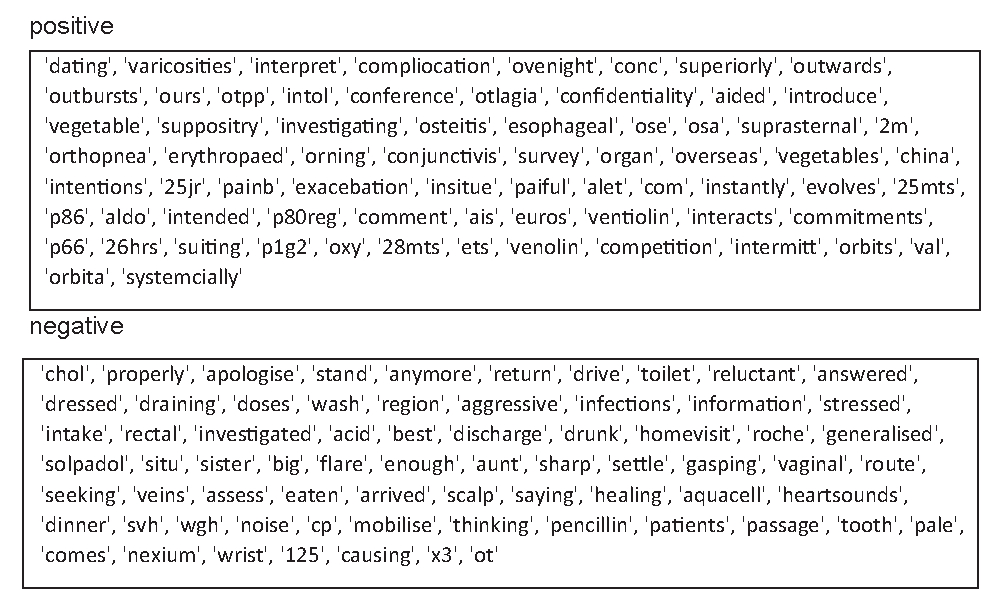
\includegraphics[scale=0.7]{word-tf-idf-unpreprocessed.pdf}
%       }
%      \caption{Top seventy tokens measured using TF-IDF}
%      \label{words-tf-idf-nonpreprocessed}
%   \end{figure}


%HOLD ON A SECOND! Naive Bayes\index{Naïve Bayes} USES TOP 100 WORDS? WELL THE TOP 70 WORDS FROM BOTH POSITIVE AND NEGATIVE CASES ARE VIRTUALLY IDENTICAL - SO WHAT... WHAT COULD IT POSSIBLY BE USING TO DERIVE AN ACCURATE RESULT IN RELATION TO TRUE POSITIVES? Lower the number of top words to 10, then to 1, to see how it does. If It still does well it is clearly cheating. Report most significant features.




%There's significant divergence between the TF-IDF tokens for positive and negative cases, as shown in Figure \ref{words-tf-idf-nonpreprocessed}. This would appear to augur well for predicting these cases. However, there are nevertheless significant issues with the highly ranked lexemes; perhaps somewhat intuitively indicated by the fact that clearly misspelled words (like `compliocation' or `pencillin') have ranked so highly. The OOHC\index{Out-of-hours Health Care} context of the data collection makes TF-IDF as a measure a little more problematic as repetition within case FTN is specifically avoided due to both temporal and comprehension considerations, while important measures may be relatively routine, thereby undercutting their apparent importance within the corpus as a whole. TF-IDF failed to produce any useful results with the classifiers, consequently the table below will relate results using most frequent terms, excluding stop-words.    




\subsubsection{Predictive performance}



 
 
 \begin{table}[h]
 \begin{center}

    \ra{1.4}
   \caption{Classification using bag-of-word\index{Bag-of-words representation} model.}
\begin{tabular}{|l|c|c|c|c|}
\hline
            & \textbf{Naive Bayes\index{Naïve Bayes}} & \textbf{SVM} & \textbf{RF} \\ \hline
Accuracy    & 0.26 $\pm 0.51$                & 0.66 $\pm 0.385$     & 0.68 $\pm 0.045$        \\ \hline
PPV         & 0.89 $\pm 0.53$               & 0.52  $\pm 0.459$    & 0.37 $\pm 0.015$            \\ \hline
NPV         & 0.24 $\pm 0.019$               & 0.49 $\pm 0.412$     & 0.69 $\pm 0.044$           \\ \hline
TPR         & 0.013 $\pm 0.001$               & 0.01 $\pm 0.0049$     & 0.006 $\pm 0.001$           \\ \hline
\end{tabular}
\label{table:ml-classification-bow}
 \end{center}
\end{table}

The results for the BOW model using the top 100 words can be seen in Table \ref{table:ml-classification-bow}. The average depth of the RF was 31.5. Naive Bayes\index{Naïve Bayes} in this instance was strongest at detecting true positives, while the RF algorithm was strongest at detecting true negatives (and consequently exhibited the best accuracy of the three algorithms tested).  

Owing to Naive Bayes\index{Naïve Bayes}' high PPV when using BOW\index{Bag-of-words representation} data, and high NPV when using parameterised data, experimentation combining both sets of data were used with this algorithm, in the event that some sort of equilibrium between true positive and true negative prediction could be attained. However, this combination merely furthered the algorithm's bias towards true negatives, with an average PPV score of 0.25 $\pm 0.47$ , and average NPV score of 0.89 $\pm 0.23$  when using this hybridised dataset.


\subsection{Summary}
\label{C}

Attempts to classify cases using more traditional machine learning techniques provided, at best, what could be described as modest results. While the lion's share of valuable information in relation to cases resided within FTN, performance of the algorithms using free text was not significantly superior to results borne from parameterised data. These results provided useful baselines from which to work, and indicated that classification using either textual data or paramaterised data would be theoretically possible. What these results did not provide was any indication the extent to which context could play a role in the use of FTN data. Although variants of the machine learning approaches taken above could theoretically provide improved performance (e.g. multinomial Naïve Bayes \cite{meftouh2019smart} or kernal based SVM), ultimately the decision was taken to focus on attempting to classify patients using FTN data by applying an artificial neural network model.



\section{Artificial Neural Networks}
\label{section:ANN-(theory)}
%\subsection{Motivation} 
When approaching the use of FTN; while the most important lexemes present in the corpus could hypothetically be extracted from cases for any classification purpose, such a position raises the question of how one would define what was, and was not, a significant lexeme in the first place. 

Intuitively, medical terms would seem to possess more importance in classifying cases. After all, physicians base their entire professions around the use of signs, symptoms, and histories of prescriptions and morbidities in their assessment of cases (though it should be noted that it would be virtually unheard of for doctors to actually provide a diagnosis based solely on textual information). Notwithstanding the conceptual soundness of this idea, the actual quality of the notes put paid to notions of using NER to this end. Typographical errors, widespread use of contractions, and a plurality of forms that different entities could take made the idea of using a predefined list of terms fundamentally unsound as a means of extracting useful features (at least in isolation).

A more general point is that this difficulty is present even if one presupposes that one's intuition concerning a certain type of word is correct. By this, it means that while it is reasonable to assume that the occurrence of symptoms and diseases in the text are significant (because they would in the context of diagnostics performed by humans), this does not necessarily mean that these particular terms (if one could even find them) are the only, or even the most important features present to solve the thesis problem. As has already been established in Section \ref{section:frequent-users-rr}, there is no accepted set of characteristics to define frequent users. As such, feature selection based upon human reasoning is, in this context, rendered somewhat moot. 

The last point ties into the choice of Artificial Neural Networks (ANNs\index{Artificial Neural Networks}) for the purposes of FTN classification. ANNs\index{Artificial Neural Networks} have in recent years been increasingly applied in natural language contexts and specifically, have had proven applicability in relation to data that has traditionally proven problematic in probability analytics and machine learning \cite{goldberg2017neural}. A particular consideration is the present context, whereby the chosen machine learning application must itself be able to learn from a sparse dataset what features represent strong information gain. Because of both the high volume of features (that is to say, unique words) and relatively high volume of data available to train models, ANNs\index{Artificial Neural Networks} presented a logical step in attempting to classify frequent user cases using FTN. 


The actual choice of neural network architecture was non-obvious. So too was the choice of data representation. Consequently an exhaustive series of tests were conducted to find to most suitable combination. It was also initially uncertain whether FTN alone or some combination with parameterised data would be prove optimal. However, before considering the methodology adopted to try and develop a solution, let us first look at what is meant by both Neural Networks in general, and specifically how recent research has appropriated them for FTN classification.  

Artificial Neural Networks are loosely modelled on their biological equivalent, and are constructed as a collection of neurons (or perceptrons) \cite{rosenblatt1957perceptron} organised in a sequence of one or more hidden layers \cite{goldberg2017neural}. Typically these networks are multiple layers deep (hence the relatively redundant term of `deep learning') where neurons receive as input the neuron activations from the previous layer \cite{rumelhart1988learning}. Neuron activations perform a weighted sum of the input typically followed by a non-linear activation function. While weights are essentially composed of random values to begin with (though the manner in which these values are generated differs depending on initialisation method used) \cite{steinwart2019sober}, backpropagation is typically a method used to adjust the connection weights to minimise the error during learning \cite{rumelhart1988learning}. 

Activation functions to find non linear error gradients can thus be used in tandem with backpropagation to find complex patterns in data. The updating of weight values is performed by an optimisation algorithm \cite{goodfellow2016deep}. However, there are multiple different activation functions and optimisation algorithms that one may use to this effect. While different activation functions and optimisation algorithms have different strengths and weaknesses, it is hard to justify an \textit{a priori} choice with relation to these components \cite{wolpert1997no}. 

Multi-Layer Perceptrons (MLP\index{Multi-Layer Perceptrons}) are neural networks with more than one layer while Convolutional Neural Networks (CNN\index{Convolutional Neural Networks}) are, simply put, neural networks that use convolution in place of general matrix multiplication in at least one of their layers. Convolution is defined as follows

\begin{equation}
s(t) = (x*w)t = \sum_{i=-\infty }^{\infty} x(i)w(t-i) 
\end{equation}

\textit{W}here \textit{x} is a vector of inputs, \textit{w} is a vector of weights, \textit{i} is an index variable, and \textit{t} is time (or window) \cite{goodfellow2016deep}.

CNNs may have pooling layers to perform non-linear downsampling. CNNs are exceptionally popular in vision recognition tasks, but as will become apparent, have had significant recent application in FTN contexts. 









Recurrent Neural Networks (RNN\index{Recurrent Neural Network}) are different from both MLP and CNN in that MLP and CNN are both feed-forward networks, in the sense that the connections
between neurons do not form cycles or loops. Feedforward networks make an assumption of independence between inputs, whereas Recurrent Neural Networks, as the name may suggest, have a looping mechanic, in the form of at least one feedback connection \cite{rumelhart1988learning}. This allows this type of architecture to treat the interdependence of sequential data. A consequence of this is that while CNNs may be able to consider the immediate context of input (for instance a local group of pixels or characters), they cannot understand temporal connections. A major limiting factor for RNN\index{Recurrent Neural Network} is that traditional, fully connected RNN\index{Recurrent Neural Network} tend to suffer from both vanishing and exploding gradients as weights are backpropagated through the recursive layers (where the model may forget earlier input, or be subject to instability) \cite{goodfellow2016deep}. The most common method to solve this deficiency is the use of a gating mechanic. 











 \section{Approaches}
\label{section:ann-approaches}

%Multi-Layer perceptrons do not take context into account

%Convolutional Neural Networks (CNNs) mix together partial information gathered from what it's looking at. 

%Recurrent Neural Networks repeat

%Gating can be used to



The use of machine learning in relation to medical data is by no means new. However, free-text\index{free-text} has proven a problematic source of features for classic machine learning techniques. Even when advanced feature extraction methodologies are employed, the inherent noise and heterogeneity of medical natural language remains an issue. Current research within medical informatics have begun to broach ANNs\index{Artificial Neural Networks} for use with data from Electronic Health Records in order to overcome these challenges. 

Issues can arise when establishing ground truth in analysis. If training data has to be generated manually by domain experts, this often results in relatively small datasets, which typically provides a poor basis upon which to use deep learning methodologies \cite{gehrmann2018comparing,geraci2017applying,yao2016convolutional}.  While this thesis can avoid this issue, particular to hand-curated datasets, as discussed in Section \ref{section-rr-medical-text}, there nevertheless is a ceiling on the volume of data that can be used in training a neural network model, owing to the fact that the classification system being developed specifically concerns outlier cases. 

However, the actual use of neural networks in conjunction with EHR\index{Electronic Health Record} has displayed wide variance in contemporary research. For instance, some researchers maintain feature extraction techniques, and use neural networks for classification purposes using these extracted features, while others use neural networks for the purposes of feature transformation, and have other types of machine learning algorithms use these features. The architectures and designs of the ANNs\index{Artificial Neural Networks} similarly are multivariate, with no single structure proving the de facto standard across extant research.

Geraci et al. for instance use MLP\index{Multi-Layer Perceptrons} as part of H2O.ai's Deep Learning platform \cite{geraci2017applying}. Similar to the objectives of this thesis, Geraci et al. seek to produce a binary classification of patients, in their case, as either suitable or unsuitable to be participants for a study on youth depression. The data Geraci et al. were considering was unstructured medical textual notes with limited application of diagnosis codes. 

Geraci et al. accepted that searching using a fixed list of terms could potentially achieve a reasonably high accuracy \textit{vis-à-vis} the correct identification (or exclusion) of potential candidates. Contextual negation was also taken into account for list based searches. On very select training sets this ``brute-force" methodology could obtain 80\% sensitivity and 88\% specificity. However, as these researchers expected, this approach did not generalise, and in some cases during cross validation it achieved no better than random accuracy.

Geraci et al. were faced with a relatively small dataset, as classification had to be performed by domain experts, leaving a total of 861 patient documents with which to work. The actual features of the documents were refined into a document term matrix, with the value for each term recorded by its TF-IDF ratio. Somewhat unusually, Geraci et al. produced two separate neural network models, one which had high specificity and poor sensitivity, and one which happened to have high sensitivity but poor specificity. By combining the results of these two neural networks Geraci et al.'s model achieved a sensitivity of 75\% and specificity of 87\%. The actual structure of the neural networks was that of a three layer network, with relu activation function on hidden layers. The significant difference between the high sensitivity and specification networks was the number of nodes, with the high specificity network having 758 input nodes, with the high sensitivity network having 102 input nodes. Other aspects relating to the architecture of either network are not looked at at length.

% Unlike Geraci et al., the dataset under investigation was substantial (comprising aggregated EHR\index{Electronic Health Record} data of some 700,000 patients, of which 76,214 were used for testing purposes).

The use of neural networks using unsupervised learning for the purposes of preprosessing of features is fairly typical in NLP applications. This is increasingly common for natural language in medical domains, as can be seen, for instance in Miotto et al.'s DeepPatient classifier project which uses a denoising autoencoder\cite{miotto2016deep}. Although DeepPatient ultimately uses a RF for the purposes of classifying patients,  the use of autoencoders clearly improved the quality of the medical textual features presented. DeepPatient's preprocessing saw dramatic improvements in detection of certain disorders, over that achieved using raw text, but this was not shared uniformly. Similarly the use of unsupervised ANNs\index{Artificial Neural Networks} to produce word embeddings, typically using Google's Word2Vec\index{Word2Vec}, has been employed to improve results of systems such as the named-entity recognition described by Habibi et al. \cite{habibi2017deep}. 

Rasmy et al. use the Reverse Time AttentIoN  (RETAIN) RNN\index{Recurrent Neural Network} model for the prediction of heart disease based on the extracted information from Electronic Health Records \cite{rasmy2018study}. While this objective is similar to this thesis' planned capacity to detect frequent users, Rasmya et al.'s data does not seem to include natural language. Importantly, Rasmy et al. demonstrated the generalisability of RNNs\index{Recurrent Neural Network}, given a corpora from different hospitals, and the superior performance of the RNN\index{Recurrent Neural Network} used in such classification compared to a more traditional model such as logistic regression.

In counterpoint, C. Yao et al. use a Convolutional Neural Network (CNN \index{Convolutional Neural Networks}) in order to predict correct answers to users' questions in an online Q\&A system \cite{yao2016convolutional}. The specific structure used in this CNN \index{Convolutional Neural Networks} is inherited from the work by Yoon Kim 
%[]
\cite{kim2014convolutional}. A large amount of preprocessing of textual data is performed on the user submitted data, with an emphasis on extracting symptoms, though these features are also vectorised as word embeddings. The accuracy of the model that C. Yoa et al. create is 71\%. It is shown in this research that the quality of the predictions in this case is largely dependent upon the number of symptoms that are present in user data. 

Gehrmann et al. also use Kim's CNN\index{Convolutional Neural Networks} architecture to attempt to identify particular patient phenotypes from patterns discovered in their medical notes \cite{gehrmann2018comparing}. In particular, as is the case in the research in this thesis, specific emphasis was placed on the identification of ``frequent flyer" patients; that is to say, patients that have an unusually high amount of contact with the healthcare facility in question. Due to the necessity of manual annotation, the dataset in Gehrmann et al.'s research was small, with some 1610 cases available for both training and testing purposes.    

Gehrmann et al. automatically extracted clinical features using cTAKES \cite{gehrmann2018comparing}, which were then used as the features in the CNN\index{Convolutional Neural Networks}. Like many of the other papers presented here, these features were provided to the classifier as a bag-of-words\index{Bag-of-words representation}. However, prior to their treatment by the CNN \index{Convolutional Neural Networks}, the words were transformed into word embeddings using Word2Vec. The CNN \index{Convolutional Neural Networks} achieved a high F-score across all tests, though results differed significantly, depending on the specific phenotype being tested. 


The use of unsupervised artificial neural networks\index{Artificial Neural Networks} to preprocess data is well established, and improvements seen in the quality of features derived from unstructured medical text is similar to that observed in other natural language domains \cite{miotto2016deep}. The use of some type of ontology to attempt to improve features is also sometimes seen \cite{gehrmann2018comparing}. The actual quality of unstructured medical text can vary wildly (both between different datasets and often within the same dataset). If individual cases are being classified, both the volume of data in individual cases, and the quality that this data is presented may form a limiting factor for the effectiveness of any classification algorithm \cite{yao2016convolutional} .

\begin{figure}[htbp]
   \begin{center}

 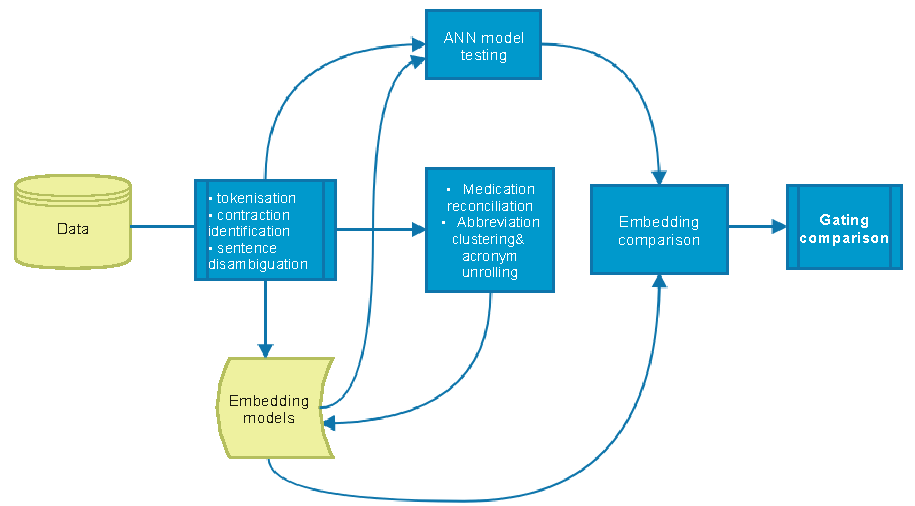
\includegraphics[width=1.0\textwidth]{Figs/scheme-development-plan-.pdf} 

 \caption{High level overview of system development.}
 \label{fig:development-plan}
  \end{center}
\end{figure}


%Similar to C. Yao et al's solution

All of the literature discussed above shows the potential strength of artificial neural networks\index{Artificial Neural Networks} in connection with EHR\index{Electronic Health Record}. However, while many of these papers compare artificial neural networks\index{Artificial Neural Networks} with other machine learning methodologies, less focus is placed on the specific type, parameters, or hyperparameters of the artificial neural network used within the scope of their analyses. 




%Cut and paste the related research from chapter 5 in here after the initial section on ANNs\index{Artificial Neural Networks} .... possibly Free-Text use of Deep Learning


A high level depiction of the methodology adapted in determining the optimal combination of neural network architecture and data representations can be seen in Figure \ref{fig:development-plan}. Note that this figure is created retrospectively (when it was already determined that a Neural Network with gating mechanic would be most ideally suited to the problem). \hl{The preprocessing steps were not entirely linear, as some processes were mutually dependent. For instance, contraction identification was necessary for effective sentence disambiguation, and sentence disambiguation was necessary for training of word embedding models. To elaborate on this point, distinguishing between full stops that formed part of contractions, and those that indicated the ends of sentences was integral to the development of training data for the generation of word embeddings.  However, the word embedding model was necessary for finding many of the long forms of abbreviations used within the corpus. The act of preprocessing itself necessitated the retraining of word embeddings to cope with the altered textual data within the corpus.} Figure \ref{fig:development-plan} also depicts the testing of the competing models of ANN\index{Artificial Neural Networks} initially considered, namely Multilayer Perceptrons, Convolutional Neural Networks, and the use of gating in the context of Recurrent Neural Networks. 








%Results in the literature suggest that artificial neural networks, particularly those which feature deep neural layers, have strong predictive power and generalize well in relation to unstructured textual data.

%\subsection{Aim}






\section{Summary}


This chapter has established the non-trivial task of attempting to classify frequent users. Although different ML approaches to classifying patient cases had diverse results, it would be hard to declare any particular algorithm as obviously superior. Nonetheless it is clear that features present in the dataset can be used to classify patients. Given the challenging nature of the data, artificial neural networks\index{Artificial Neural Networks} appear to be good alternative to more traditional ML approaches. However, the network most appropriate to the task at hand is initially unclear. Existing research into use of FTN has not displayed any single network type as indisputably superior. Furthermore, given that the specific dataset under investigation in the course of this thesis has not been subject to any prior ML research, evaluation of different methods of data representation would appear warranted.     




 \chapter{Preprocessing}
 \label{chpt-preprocessing}
 \nomenclature[1]{INN}{International Nonproprietary Name} 
 \nomenclature[1]{BAN}{British Approved Name}
 \nomenclature[1]{USAN}{United States Adopted Name}
 
 
 
 \section{Introduction}
 
In order to improve classifier performance we sought to develop preprocessing methodologies that would improve the quality of text which would be developed into word embeddings. The primary goals of this work was to provide feature reduction and error correction. 

The issue to be addressed in preprocessing was the noisy, high dimensional recording of two different types of potentially useful terms within the FTN: namely that of medications and contractions. We detail in this chapter the issues found in relation to these two aspects of the FTN, the approaches we used to address these problems, and the ultimate performance and limitations of the methodologies that were developed.



The hypothesis was that providing more abstract versions of terms in text would ultimately improve classification capacity. Alternatively, some high value terms could be hidden within acronymised forms. 

\hl{
The methodologies discussed in this chapter use the entire volume of free-text data contained within the corpus, as described in Section} \ref{section:free-text-description}, for all training and text transformation operations. The contents of this chapter were in part published in IADIS 2017 `Abbreviation and Acronym Identification and Expansion Within Medical Health Records' \cite{wallace2017abbreviation} and `Retrieval and Clustering of Medicines Within Healthcare Data Records' \cite{wallace2016retrieval} in BDAW 2016 which sought to identify means of identifying and correcting both contractions and medications in the corpus, respectively.

\section{Medication Reconciliation}
\label{section:medication-reconciliation}

As mentioned in Chapter \ref{chpt:background}, the free-text medication data in EHR\index{Electronic Health Record} is predominantly unsanitised, and its unstructured nature makes it inaccessible to other computer applications that rely on coded data in healthcare settings (e.g, electronic medication reconciliation systems), as well as clinical research that uses structured medication data, such as EHR\index{Electronic Health Record}-based \cite{kushima2012text}. Despite providing a means of reducing paper-based inaccuracy, Electronic Medical Record Management systems are still subject to human error \cite{koppel2009emr}.

Medication reconciliation is a formal process for creating a more complete and accurate list of a patient's medications for the purpose of supporting correct medication orders. Given the increasing use of EHRs\index{Electronic Health Record}, automated medication reconciliation methods have received great attention \cite{grossman2014hospital}. One particular challenge involves the heterogeneity of clinical data, which consists of both coded and narrative medical data \cite{michaelsen2015medication}.

Despite the inherent value that these terms bear, free-text medical information may contain large volumes of pharmaceuticals recorded inconsistently, both stylistically and structurally. The pharmaceuticals themselves may be incorrectly recorded, and no list of pharmaceuticals likely to recorded in a corpus may exist. The purpose of this part of the research is to develop a system that can extract drug names from this unstructured data in order that this information be available for analytical purposes, both on a population and individual basis. In this way it may be possible to provide useful and interesting inferences over large volumes of data.




This section will examine the ways in which pharmaceutical discovery can be achieved, before looking at the ways in which this thesis' methodology was implemented. The proposed solution will build upon extant research, as described in Section \ref{section-rr-medication-identification}. The methodology will focus on environmental analysis of the text and, as such, a subsection will explore the manner in which this was conducted. Finally, the results of the information retrieval and success of the clustering of such terms is analysed.   




\subsection{Problem Definition}

 While drug names tend to follow certain morphological conventions, these not only pose a problem by their sheer volume, but even presupposing that pharmaceuticals are recorded using full international non-proprietary name \\ (INN) \cite{dunne2013review}, stems used to denote drugs are syntactically so sparse as to preclude any sort of acceptable precision. Naturally, such affixes and suffixes are unlikely to relate to proprietary names under which these products are marketed, which may be the manner in which drug products are represented within the text. As such, the analysis of words, in isolation, to discover medications within the text can be discounted. 
 

Instead, an analysis of the structure of medical notes to detail the types of syntax which are likely to indicate the presence of medications will be conducted. Although the heterogeneity of free-text notes precludes certain NLP\index{Natural Language Processing} measures, developing simple syntactic patterns has the potential to accurately return medication names within such notes.

It is a primary ambition of this part of the research to deliver a system that can not only identify the proprietary, trade and generic names of pharmaceuticals, but provide also the means for incorrectly transcribed pharmaceuticals occurring within free-text notes to be automatically corrected with a high degree of precision. 


This chapter aims to discover a broad spectrum of medications, but will consider all other lexemes to be incorrect. For instance, the term ``antibiotic" would be considered to be a valid medication name (despite its generic nature) while a word like ``emulsion", which denotes a delivery method for medications, would be considered incorrect. All lexemes which denote medications, but are incorrectly spelled (for instance \textit{prendnesol} instead of \textit{prednesol}) will be considered erroneous.  

\subsection{Proposed Solution}
\label{section:prescription-solution}

Using a predefined list of drug names (namely using RxNorm\index{RxNorm}), co-occurring terms found within the text will be collected, excluding stop words.  The highest frequencies of co-occurring lexemes will next be compared against one another in order to develop well defined environments within which medications are likely to be present. 

Once structures which telegraph the presence of medication details have been defined, suitable structures will be used to collect lexemes which may represent medications.  The data collected will exclude common English words and lexemes less than three characters in length (as the latter are too short to relate to pharmaceutical names). The accuracy of the pattern used to discover candidate medications names will underpin the precision of the overall program, as both unrelated medical words, and misspelled words that do not relate to medications are otherwise likely to be returned by this process.

\hl{Data relating to common English words was derived from a truncated version of SCOWL}\index{Spell Checker Oriented Word Lists}, of size 35 (the recommended `small' size of the SCOWL repository, where `size' is synonymous for how common the specific lexemes are)\cite{atkinson2004spell}. This dataset, reportedly around 7.6\% of the total volume of SCOWL lexemes, totalled some 50,000 words. The rationale for using this particular subset of the SCOWL dataset was its purpose in excluding common, non pharmaceutical lexemes in the following tasks. A much larger version of SCOWL could potentially run the risk of excluding some true positive pharmaceutical candidates.

By searching all other text for occurrence of the collected words, a dataset of pharmaceuticals and their frequency within the EHR\index{Electronic Health Record} can be established. The collection of drug and product names above is guaranteed to return many errors, both typographical and cognitive in nature, where users have entered the names of products they are describing incorrectly. Common English words which have been misspelled, and domain-specific terms alike may also hypothetically be collected in this process. Furthermore, terms that are four characters in length are overwhelmingly likely to represent domain-specific acronyms, or product name contractions. However, by analysing both the frequency of occurrence and morphological similarity of the terms collected, it is intended that the program will automatically correct these errors.
 




%\begin{figure}[!t]
%\centering
%\includegraphics[width=2.5in]{workflow.png}
%% where an .eps filename suffix will be assumed under latex, 
%% and a .pdf suffix will be assumed for pdflatex; or what has been declared
% \DeclareGraphicsExtensions.
%\caption{Overall program structure.}
%\label{workflow}
%\end{figure}



\subsection{Methodology} 
 \label{section:pharmaceutical-retrieval-methodology}
 
%The data provided, which had previously been anonymised, was cleaned of duplicate entries and tokenised. The preprocessed text was analysed for sentence structures which would indicate the presence of prescription details. Terms in proximity to numerical tokens succeeded by prescription related lexemes were collected as candidate names.

By taking the list of drugs presented within RxNorm\index{RxNorm} the frequencies of all co-occurring words were recorded. Co-occurring words could appear immediately before or after the name being searched, provided that it was not interceded by punctuation (newlines, periods, etc.). Stopwords were excluded from this process using the twenty five semantically non-selective words which are common in Reuters-RCV1\cite{sanderson2010christopher} \footnote{This list can be viewed in Table \ref{table:app-stopwords} in the Appendices.}.
 A very small stopword list was demanded for this task, in order to avoid accidentally filtering important neighbouring terms during analysis, hence the choice of this particular list. 

Having collected the frequencies of co-occurring words, work was begun on creating a co-occurrence network in order to identify structures within the text that pharmaceuticals are likely to be found. Analysis of the interconnection between the top forty terms was conducted. Interconnection was determined by simultaneous presence of terms on the same line of text within the corpus of free-text notes. 

While mutual information may theoretically have produced more accurate results in this regard \cite{nakagawa2003automatic}, this process was merely exploratory in nature, whereby the identification of medication contexts was a means to an end to discover medication candidates. These candidates in turn would be leveraged to identify further candidates. 

In order to eliminate the long tail of infrequent terms, the co-occurrence network eliminated nodes that failed to have any edge with a weight within the top half of occurrences. This approach was appropriate given the immediate demand to identify the most typical environment within which medication terms might occur. Finally, modularity of the network was conducted, separating the network into three distinct classes using Blondel et al.'s clustering algorithm \cite{blondel2008fast}, as can be seen below in Figure \ref{network-drugs}. Despite mutually exclusive clusters, very strong connections between terms in one cluster and terms in another cluster may exist  (e.g. between `pain' and `po').

The orange coloured community represents paediatric related contexts. Nurse triage staff answering paediatric related cases may advise the use of non-prescription based medicines in many cases in order to ease the symptoms relating to the child's complaint. This context consequently tends towards a relatively limited number of medications which occur in high frequency. This can be observed in the presence of a pharmaceutical name which has actually appeared within this cluster (namely `calpol').

The second community identified (green) is a more generalised context relating principally to initial contact between a patient and phone operator where non-specific details may be related. While the lexemes in this group have a relatively strong correlation with medications, and a particularly high correlation with one another, the high variance of types of information related in the proximity of these terms augurs poorly for the precision of medicine based information retrieval. 

Prescription details (purple) closely mirror their real-world handwritten equivalents, both in terms of register and structure. As such, the invocatio of the praescriptio typically contains weights and measures \cite{hadavsova2009practicals}. This generates a consistent pattern of drug or product names, succeeded by measurements (that may change temporally), which may be followed by some temporal value. These prescription details may be singular or composite.

When looking for non-lexical co-relation with the different classes, prescription based words had a particularly strong relationship with numerical elements. Lexemes belonging to the prescription class had a total of 100,669 numerical co-occurrences compared with 3,654 for general and 12,954 for paediatric contexts. 

Taking account of the semantic ordering of prescription related terms, certain patterns became apparent, with particular terms tending towards different relative positions. When grouping the terms by meaning (relating to quantifiable and temporal specifications), the most common semantic structure was for numerical tokens to be followed by quantification and temporal tokens, in that order (with some 25,618 occurrences). The second most common structure was for numerical tokens to be followed simply by quantification tokens (with some 16,617 occurrences).  

Using this as a means by which to proceed, the preprocessed text of the corpus was analysed for sentence structures which would indicate the presence of prescription details. Terms in proximity to numerical tokens, succeeded by prescription related lexemes in the order hitherto observed, were collected as candidate names. Terms which were within SCOWL \index{Spell Checker Oriented Word Lists} were excluded, while those less than three characters in length were discarded in favour of the nearest suitable lexeme. 



    \begin{figure}[!ht]
      \centering

      \includegraphics[scale=0.5]{network-drugs.pdf}
      
      \caption{Undirected graph of context relations.}
      \label{network-drugs}
   \end{figure}


%In order to determine the accuracy of the program an exhaustive search was conducted through various media to ascertain whether each of the recorded candidate names was a correctly written pharmaceutical. 

Following the collection process, a frequency was taken of all collected candidate names within the entire training corpus. This was done so that the recorded frequency would reflect the general preponderance of candidate names within the text, not limited solely to the context of prescriptions.

Of the terms collected, names that were were exactly four characters in length overwhelmingly represented false positives or abbreviated forms of drug names. Contracted forms of drug names typically have very large edit distances from their full length versions, so a specific process of contraction inflation was developed. This process analysed the longer candidate medication names for a potential match, based both upon length and morphological similarity. In the event of a conflict, the full-length candidate name with a greater frequency was chosen. Any term which ultimately found no suitable match was removed from the list of candidate names.

Finally, the edit distance between candidate pharmaceuticals was tested using an implementation of the Levenshtein distance string metric \cite{schulz2002fast} (see \hl{Figure} \ref{euclid}). The hypothesis was developed that supposed that the edit distances would be predominantly short between incorrect pharmaceutical entries and their correct versions, and that, as a general principle, incorrect edits would necessitate longer edit distances \cite{hodge2003comparison}.  This was implemented using varying distance criteria, and the results recorded \hl{(see Table} \ref{table:lev-distance1}).

%INSERT MATHEMATICAL FORMULA INSTEAD OF PSEUDOCODE HERE


\begin{figure}
\begin{algorithmic}[1]
\Procedure{editDistance}{$s1,s2$}
\State $a[i,k] =0$
\For{$i = 1 \to  |s1|$}
\State {$a[i,0] = i$}
\EndFor
\For{$k = 1 \to  |s2|$}
\State {$a[0,k] = k$}
\EndFor
\For{$i = 1 \to  |s1|$}
    \For{$k = 1 \to  |s2|$}
    \State {$a[i,k] = \min\{a[i-1,k-1]+$}
    \If{$(s1[i]=s2[k])$}
        \State{$0$} 
    \Else 
    \State{$1$} 
    \EndIf
    \State {$a[i-1,k]+1, a[i,k-1]+1$}
    \EndFor
\EndFor

\State \textbf{return} $a[|s1|,|s2|]$
\EndProcedure
\end{algorithmic}
\caption{Levenshtein distance.}\label{euclid}
\end{figure}


%\subsection{Results}

Candidate medications were collected from the dataset through the identification of prescription details. This resulted in 3,778 candidate pharmaceutical names being obtained. When searched for through the entire corpus, it was found that these candidate names related to some 460,232 occurrences within the entire text.  

However, of these candidate names, only 896 terms were correct (being both actual pharmaceuticals, and correctly spelled). Of the 2,893 incorrect candidate names, the vast majority represented incorrectly spelled drug names, with only 98 falling into other categories (predominantly relating to abbreviated forms of drugs and routes of administration). Incorrect terms accounted for roughly half the population of candidate instances within the corpus (152,500 versus 155,295).


\subsection{Abbreviation Inflation}

A very simple means of dealing with abbreviated pharmaceutical names was devised that would attempt to match short candidate names that were collected during the information retrieval task detailed in Section \ref{section:pharmaceutical-retrieval-methodology}. This program would try to find another candidate name, of which the proposed abbreviated pharmaceutical was a substring, and delete the proposed abbreviation if no match was made. This program was run on the 86 candidate names which were 4 characters in length. This resulted in one false-negative being deleted (a drug with some 569 occurrences in the corpus), and two false-positives, where drugs were wrongly inflated to larger forms (accounting for 17 occurrences together). 

Twenty-eight true-positives were identified and correctly inflated (totalling some 2990 occurrences), although two of these candidates were inflated to words which were themselves incorrect candidates: namely nebulizer (61) and suppository (52), both of which are routes of administration rather than pharmaceuticals.

An additional fifteen abbreviations (totalling 89 occurrences) were incorrectly identified as being pharmaceutical abbreviations and were added to the count of extant drugs.

Forty-two abbreviations were deleted, thirty eight of which were correctly identified as being unrelated to any larger form, such as `meds' and `stat'. These thirty-eight abbreviations which were deleted accounted for a substantial population, relating to 108531 occurrences within the corpus. The four abbreviations which were incorrectly deleted were somewhat aberrant in that their abbreviated forms did not match their full length counterparts (such as penv and phenoxymethylpenicillin). These false-negatives related to sixty-five occurrences in the corpus.

The abbreviation-inflation described above had a marginal effect on the average length of candidate names, whereby an increase was observed of the plain average of names, where candidate names are treated as a set, from 8.86 to 8.97, and an increase of the weighted average, where candidate names are treated as a multiset, from 7.046 to 8.03. However, this process had a substantial impact on the standard deviation of incorrect candidate names, decreasing from 1439.264 prior to inflation, to 132.827 afterwards).

\subsection{Edit distance}
\label{section:medication-collection}

Once the abbreviation inflation had been concluded, the edit distances of all candidate names were tested against one another using a varying distance parameter (see Table \ref{table:lev-distance1}). The aim of this comparison was to not only remove incorrect candidate names, but to also add the count of incorrect candidates to their corrected versions, where applicable. 

It was expected that a higher edit distance would result in higher true positive changes, but with a corresponding rise in false positives. As it was unclear, \textit{a priori}, what kind of ratio this would have, the results from edit distances between one and four (inclusive) were recorded (Table \ref{table:lev-distance1}). 

Corrections from one true (\textbf{t}) form to another true form is considered fallacious, as this is more likely to result in a pharmaceutical being corrected to an unrelated pharmaceutical. Yet, even if the correction is to a related product, this represents a form of generalisation not specifically sought within the scope of this research. Alteration of correct pharmaceutical names to incorrect versions are in particular to be avoided, as this not only removes a correctly identified medication from our list, but gives undue weight to incorrect entries. Corrections from one incorrect entry to another are predominantly beneficial, as not only is an incorrect entry removed from the list in this process, but it is possible that the form to which it has been corrected may act as an incremental step towards the appropriate spelling of the pharmaceutical. 





\begin{table} [ht]
%% increase table row spacing, adjust to taste
\renewcommand{\arraystretch}{1.6}
\setlength{\tabcolsep}{0.7em}
% if using array.sty, it might be a good idea to tweak the value of
% \extrarowheight as needed to properly center the text within the cells
\caption{First iteration of edit distance.}
\label{table:lev-distance1}
\centering
\begin{tabular}{@{}c|c|c|c@{}}
\toprule
\textit{distance}   & \textbf{f$\rightarrow$t} & \textbf{t$\rightarrow$ t} & \textbf{t$\rightarrow$ f} \\ \midrule
\textit{\textbf{1}} & 1587                     & 47                        & 19                        \\ \midrule
\textit{\textbf{2}} & 2572                     & 137                       & 36                        \\ \midrule
\textit{\textbf{3}} & 2483                     & 394                       & 56                        \\ \midrule
\textit{\textbf{4}} & 2757                     & 821                       & 45                        \\ \bottomrule
\end{tabular}
\end{table}

\begin{figure*}[ht]
\centering
\includegraphics[width=\textwidth]{replace_drugs.PNG}
% where an .eps filename suffix will be assumed under latex, 
% and a .pdf suffix will be assumed for pdflatex; or what has been declared
\DeclareGraphicsExtensions.
\caption{Network simulation of correction decisions at a distance of two.}
\label{network}
\end{figure*}

A network representation of this process can be observed in Figure \ref{network}, where the edit distance is set to two. Green nodes represent correct candidate names, while red nodes represent incorrect ones. Node sizes represent the number of occurrences within the text.

As can be seen in Table \ref{table:lev-distance1}, edit distances of three and four had had significantly inferior performance (relative to the number of errors generated) and subsequent testing was consequently conducted using edit distances of one and two. These edit distances, visible in Table \ref{table:lev-distance2}  were executed on the previous results relating to edit distances of one or two, in order to explore whether increased accuracy might be generated by this process.






\begin{table}
\renewcommand{\arraystretch}{1.6}
\setlength{\tabcolsep}{0.7em}
% if using array.sty, it might be a good idea to tweak the value of
% \extrarowheight as needed to properly center the text within the cells
\caption{Second iteration of edit distance.}
\label{table:lev-distance2}
\centering
\begin{tabular}{@{}ccccc@{}}
\toprule
\textit{initial step}                            & \textit{second step}            & \textbf{f$\rightarrow$t} & \textbf{t$\rightarrow$ t} & \textbf{t$\rightarrow$ f} \\ \midrule
\multicolumn{1}{c|}{\multirow{2}{*}{\textit{1}}} & \multicolumn{1}{c|}{\textit{1}} & \multicolumn{1}{c|}{203} & \multicolumn{1}{c|}{9}    & 1                         \\
\multicolumn{1}{c|}{}                            & \multicolumn{1}{c|}{\textit{2}} & \multicolumn{1}{c|}{568} & \multicolumn{1}{c|}{95}   & 11                        \\ \midrule
\multicolumn{1}{c|}{\multirow{2}{*}{\textit{2}}} & \multicolumn{1}{c|}{\textit{1}} & \multicolumn{1}{c|}{84}  & \multicolumn{1}{c|}{11}   & 3                         \\
\multicolumn{1}{c|}{}                            & \multicolumn{1}{c|}{\textit{2}} & \multicolumn{1}{c|}{127} & \multicolumn{1}{c|}{45}   & 35                        \\ \bottomrule
\end{tabular}
\end{table}



The most successful route of edit distance correction involved an iterative process of correcting to a distance of two, and then correcting again to a distance of two on these results. 

\begin{table}
\renewcommand{\arraystretch}{1.6}
\setlength{\tabcolsep}{0.7em}
% if using array.sty, it might be a good idea to tweak the value of
% \extrarowheight as needed to properly center the text within the cells
\caption{Pharmaceutical test results.}
\label{table:pharmaceutical-testing}
\centering
\begin{tabular}{@{}lccc@{}}
\toprule
                  &                           & correct edit & incorrect  edit \\ \cmidrule(l){3-4} 
initial incorrect & \multicolumn{1}{l|}{33.1} & 84.78        & 2.17            \\
initial correct   & \multicolumn{1}{l|}{76.9} & N/A          & 2.15            \\ \bottomrule
\end{tabular}
\end{table}

This process left 728 correct pharmaceutical names out of a total of 977 candidate names. However, a substantial number of these medications appeared only once within the entire corpus. These 200 single instance candidate names, which were predominantly incorrect (146 false to 34 true) could be discounted as outliers and removed. This left 685 true to 95 false candidate names: representing an overall accuracy of 88.15\%. When taking volume of occurrence into account, the retained candidate names represent an accuracy of 93.6\%

This final result represents an over 57\% rise in the precision of candidate names, from an accuracy of only 30.97\% of \hl{candidate pharmaceuticals collected during the initial information retrieval detailed in Section} \ref{section:pharmaceutical-retrieval-methodology}. Of the initial 896 correct candidate names identified, 76.45\% were retained. However, if we discount outliers, this retention rises to 82.63\%. Looking at the numbers that the surviving candidates relate to, we see 359,207 occurrences, of which \hl{334,599} relate to correct pharmaceutical names. However of this number  9870 instances relate to one correct pharmaceutical being wrongly corrected to another.

Taking a random sample of 200 records that were hand annotated by a domain expert for testing purposes (Table \ref{table:pharmaceutical-testing}), the program's training data achieved an 82.56\% recall. Of the pharmaceuticals correctly identified, 33.1\% were incorrectly spelled or written, of which 84.78\% were successfully corrected by the program, 15.21\% were unchanged and 2.17\% were incorrectly changed. Of the 76.9\% of the pharmaceuticals identified which had been correctly spelled, a further 2.15\%  were erroneously changed.

\subsection{Discussion}

The most apparent finding from the results is that automatic correction of pharmaceuticals necessitates very large volumes of data for accurate results. The greater the volume of data presented, the more likely that drugs will appear in the context of prescriptions and be caught by the information retrieval methods designed specifically to parse these structures. Moreover, the greater the volume of data collected, the easier it is to identify false positives and incorrectly recorded pharmaceuticals. 

While the contextual analysis performed relatively well in excluding unrelated domain-specific terminology from results, 11 of the 777 final candidate pharmaceutical names were such terms (for instance `paediatric' and `suppos'). A possible solution to this would be to clean final results with a more extensive dictionary than that used in the course of this chapter. It would not be advisable to use this larger dictionary to filter pharmaceuticals at the beginning of the collection process, as both abbreviations and variant spellings were clustered on these terms in the course of the program. However, the fact that 7 of these terms tend to appear in quite close proximity to prescription details may indicate a means of exclusion through contextual analysis. The 18 incorrect candidate names which represent misspelled English words (such as `injeciton', `depressent', and `strenght') may potentially be targeted in a similar manner.

The program is fundamentally dependent on users predominantly writing correct versions of pharmaceuticals, and cannot account for particularly prevalent cognitive mistakes \cite{sessions2006effects}. For instance, a majority of users believed that amoxicillin was spelled amoxycillin in the corpus. This had the effect of inadvertently causing the correct version of the drug name to be clustered on the incorrect version \footnote{While not very relevant to our purposes of using this preprocessed data for classification of frequent users, this taxonomic error was automatically fixed in Section \ref{section:dbpedia}}. 

%Finally, in a handful of cases contracted forms of pharmaceuticals were longer than was originally expected, e.g. `fluclox' (for `flucloxacillin'). A relatively trivial solution is to automatically inflate candidate names which are affixes of longer alternatives. 

While a conservative ceiling on edit distances will reduce the identification of false negatives \cite{jupin2012understanding}, there is no means to eliminate all possible false negatives without recourse to some sort of ontology.

Using a predefined list of pharmaceuticals to develop a topographical understanding of context has proven a suitable means to discover pharmaceutical environments. However, while context has clear application in identification of medications within free-text notes, a more syntactically sensitive approach may yet yield stronger results in terms of both recall and precision. Nevertheless, the process exhibited in this chapter has strong performance in both these categories. In particular, the capacity of the method described to discover hitherto unknown pharmaceuticals has obvious application. Non-trivial exclusion of false-positives is an ongoing concern. Furthermore, the method described does not itself provide any information about the relationships of true-positive pharmaceuticals to one another, and many different products may be recorded that have similar, or even identical functions.     



\subsection{\hl{Feature Reduction}}
\label{section:dbpedia}


Reduction of synonymous features is a useful step in the preprocessing of data prior to its use in machine learning and data mining applications. One of the most important features in clinical free text is the prevalence of pharmaceutical names. These names vary from local brand names to internationally recognised drug names. Local brand names, while understandable to people living in the area in which the data is being recorded, have the potential to obfuscate the general type of medication that is being discussed. As such, a means to abstract pharmaceuticals to a higher level, from an ontological point of view, would likely reduce ambiguity within text.

To this end the viability of many official pharmaceutical repositories, such as RxNorm \index{RxNorm} \cite{nelson2011normalized}, were examined. This was done with the hope of being able to resolve these ambiguous names. However, many of these repositories tended to feature relatively limited capabilities in mapping of proprietary to non-proprietary names, and a conspicuous absence of the types of local trade names which are specific to the environment in which our corpus was created. Consequently, these repositories provided little applicability to our needs. Instead, the ontological representation of Wikipedia, namely in the form of DBpedia\index{DBpedia} \cite{lehmann2015DBpedia}, provided a viable platform for this type of feature reduction.


One of Wikipedia's core tenets is that different pages should not exist on the same topic. Specifically, it has a policy against content forking where redundant information may be produced. Duplicate content may be deleted, or merged with preexisting articles. In order to aid both navigability and search optimisation, redirects exist to point synonymous terms (or variant spellings) to a particular article. Specifically in relation to drugs, Wikipedia's policies state that article titles should be their International Nonproprietary Name (INN) \cite{kopp1995international}, while other identifiers (such as The British Approved Name (BAN) \cite{british2002british} or United States Adopted Name (USAN)\cite{boring1997development} variants)  may also be mentioned in the lead section of articles. Consequently, proprietary and common names of pharmaceuticals typically exist solely as redirects to articles listed under the product's INN.

While DBpedia\index{DBpedia} is a structured hierarchical form of Wikipedia, it maintains metadata relating to the type of redirects described above (in accordance with the Linked Data principle \cite{bizer2011linked}) . Pharmaceutical names have previously been collected from our corpus and cleaned using information retrieval methods and clustering in Section \ref{section:medication-collection}. Using this list of pharmaceuticals against the DBpedia\index{DBpedia} API, XML featuring the labels relating to the respective medication articles hosted on Wikipedia could be derived. \hl{Using this methodology the number of distinct pharmaceuticals could be significantly reduced within the corpus through substitution with the parsed XML labels.} 


\begin{figure}[h]
   \centering
   \begin{tabular}{@{}c@{\hspace{.5cm}}c@{}}
 \includegraphics[page=1,width=.80\textwidth]{druggy3.pdf} & 
   \end{tabular}
  \caption{Sample identification, lexical correction, and transformation using DBpedia\index{DBpedia}, in relation to medications within the unstructured textual notes.}
 \label{druggy}
\end{figure}

An example of this process can be seen in Figure \ref{druggy}.  The results of this process was the reduction of pharmaceuticals from 777 distinct classes (excluding single entry medications) in the entire corpus to only 309 (though 8 pharmaceuticals were disambiguated to two separate classes)\footnote{While disambiguation was not behaviour particular sought after in this process, it was not, strictly speaking, in error.}. Moreover, only 189 pharmaceuticals remained entirely unchanged,  with the remaining 588 being resolved to a more generic variant.




%SHOW THE PROCESS OF CHANGING A SINGLE DRUG NAME TO GENERIC FORM




A perennial issue in relation to contractions is the ambiguity inherent in potential reading, when canonical definitions are not provided in the text. Unlike scientific journals, medical free-texts typically do not provide glossaries or in-line explanations of contractions, and even where an organisation may provide guidelines concerning the use of acronyms and abbreviations; these may not necessarily be followed by individual users\footnote{ Caredoc\index{Caredoc}, as previously mentioned, does not possess any guidelines on the use of abbreviations and acronyms by its staff.}. Moreover, synonymous terms may be recorded as morphologically unique contractions. 

Semantic details proved poor at identifying contractions. However, it was discovered that contractions had a number of distinguishing syntactic characteristics within free-text. Although a number of these identifiers may exist simultaneously, at times none of these characteristics may be present as writing styles vary greatly from one author to the next. Supervised learning using the Naive Bayes\index{Naïve Bayes} algorithm over the syntactic details extracted relating to candidate contractions was successful in correctly classifying them as either true or false positives \cite{wallace2017abbrev}.

To the end of developing a system to inflate contractions to their full length forms, we approached a
number of domain specific repositories with the aim of both achieving a comprehensive list of full length descriptions, and the provision of disambiguation. The repositories used were the structured list of medical abbreviations on Wikipedia, the official list of abbreviations produced by the Irish Health Service Executive, and Acromine\index{Acromine}'s RESTful API \cite{okanohara2006improving} populated from Medline\index{Medline}. Both Wikipedia and Acromine\index{Acromine} provide disambiguated results, while both the HSE and Wikipedia lists consist of manually written entries. Comparisons across the three repositories were automatically conducted to correctly unroll the contraction candidates. 


\section{Abbreviation and Acronym Clustering}
\label{section:abbreviations&acronyms}

Feature extraction is among one of the more challenging and important NLP\index{Natural Language Processing} tasks when considering the treatment of free-text medical records. Two particular complications in performing such extraction are the ambiguity of feature identification, and the plurality of forms similar features may present themselves. Ambiguity frequently occurs because high value words or phrases may be hard to recognise in the relatively unstructured form that most clinical narratives take. A particular challenge emerges however in that many terms and phrases are contracted to abbreviations or acronyms, thereby significantly increasing the challenge posed in both retrieving these terms and identifying their meaning. Yet, this obfuscation of meaning is not the only contributing factor to the plurality of forms that similar features may exhibit. Synonymous terms may be recorded as morphologically unique contractions.

Note that, for the purposes of simplicity, this chapter is conflating both true acronyms which are pronounceable (such as AIDS), and letter sequences, (such as COPD) \cite{martin2014speech}. 

Although a number of contractions have common usage throughout the medical domain, users unfamiliar with the stylistic habits of a particular organisation may have difficulty in correctly interpreting short-hand particular to that body. Contractions may also be subject to neologisms as non-standard, emergent forms,
become spontaneously popular among individuals. It is therefore no surprise that NLP\index{Natural Language Processing} applications may struggle in correctly distinguishing contractions and their potential meaning within unstructured text. Furthermore, features which are in practical terms synonymous may easily be treated as distinct in NLP\index{Natural Language Processing} applications. As most potential features within free-text notes, with the exception of pharmaceutical entities, are recorded in some type of contracted form, these issues consequently have significant negative consequences on classifier performance, and upon knowledge discovery as a whole, within the context of
clinical text.


\subsection{Proposed Solution}

In this chapter the means that were used to identify contractions and subsequently resolve them to their full-length forms are described. To this end a text analysis system which collects candidate contractions and extracts features relating to such has been developed, based upon lexical structure and sparse
contextual details. We subsequently developed a supervised classifier to distinguish true positive acronym and abbreviation candidates from spelling errors and outlier lexemes. In the second part of this chapter we describe how we attempted to derive the long forms for contractions classified as true positives through two separate methods. The first method for correctly attributing contractions to their long forms was broached by vectorising true-positive contractions. These vectors were then compared with their semantic neighbours for syntactic similarity, with substitution taking place in the event of a successful match.

We also developed a database of long forms by analysing three separate repositories of contraction definitions. This was achieved by having a majority vote between the three repositories where conflicts arose, and by automatically parsing long forms for similarity. No long forms where chosen where consensus
between two of the three repositories could not be reached. While the first method’s approach of substituting semantic matches would only be able to find the correct
long form for abbreviations, as opposed to acronyms, this method was nonetheless given precedence over potential repository forms in order to avoid false-positive attribution of acronym definitions. It was furthermore hoped that, where a long form could not be derived, that synonymous terms may be successfully combined.

The proposed solution was to build a system to provide text normalisation by taking high value terms and, through recourse to publicly available online repositories; reduce ambiguity, remove peculiarities of the local
dataset, and rationalise the consequent extracted features. This system was to include an information retrieval and supervised learning classification of contractions, and comparison of both contractions and pharmaceuticals (two of the most important constituents to clinical free-text) with freely available third party data repositories. The ultimate aim of this was to transform features recorded in the vernacular to more generic forms. This transformation would include the expansion of contractions to their full length forms, and
feature reduction in the case of pharmaceuticals. A successful combination of these techniques would increase the value of medical text for use in NLP\index{Natural Language Processing} applications. 

\subsection{Methodology}

In initial exploration it was discovered that contractions had a number of distinguishing characteristics within free-text. Other than the fact that contractions, by their nature, tended to have short length, they could be written as letters separated by symbols, in block capitals, or potentially followed by periods. Although a number of these identifiers may exist simultaneously, at times none of these characteristics may be present as writing styles vary greatly from one author to the next. A lexeme exhibiting any of these characteristics in
isolation by no means indicates it being a contraction. For instance, some authors may use block capitals to indicate the use of a contraction, while others may habitually use block capitals for emphasis or the purposes of legibility. 

%test
\begin{figure}
\centering
\includegraphics[width=4.5in]{placeholder.png} %testucd
% where an .eps filename suffix will be assumed under latex, 
% and a .pdf suffix will be assumed for pdflatex; or what has been declared
\DeclareGraphicsExtensions.
\caption{Exponential decay of contractions, relative to frequency.}
\label{fig:abb}
\end{figure}

%Figure 1: Exponential curve of contraction candidates
\VerbatimFootnotes

Contractions were predominantly non-standard English words. \hl{ The same truncated version of SCOWL}\index{Spell Checker Oriented Word Lists}, as described in Section \ref{section:prescription-solution} (totalling some 50,000 words), was used for reference. By using regular expressions to find characters  separated by repeating symbols,\footnote{\vspace{-24pt} \begin{verbatim}     i.e. (\w+)\s+(\w\w\w)\s+\d+\s}\end{verbatim}} and retrieving lexemes that were non English words, the frequency of all non-dictionary lexemes less than six characters in length were recorded. Contractions that appeared in different forms (e.g. a+e and A\&E) were counted together. As anticipated, contraction candidate frequencies followed an exponential distribution as seen in Figure \ref{fig:abb} (y axis scale is
log\textsubscript{10}). As expected also, the vast majority of unique lexemes collected were, in fact, unintentional spelling errors. These errors greatly contribute to the long tail of candidate frequencies visible in Figure \ref{fig:abb}.

While this underpinned the value that the identification of true positive contractions would have on the process of removing textual errors, it also indicated that frequency was a key feature of true positive contractions.


\subsection{Classification}

While we made efforts to look at potential semantic structures of lexemes which represented true positive contractions, in terms of both the occurrence of vowels and consonants, and potential phonetic structures which could be derived, no consistency between true positives could be determined using such a methodology. Unfortunately, using an N-gram-Over-Context model (NOC)\cite{kawamae2016n} similarly provided little better than random results in testing, as contextual features varied wildly for different types of contractions. Instead, features of candidate contractions were extracted based upon syntactic characteristics, with the value determined by frequency. As contraction frequency distribution was exponential, with a long tail of potential candidates, frequency values were consequently discretised into quartiles. Syntactic features were related to use of case (where the context was dissimilar), composition using symbols, and symbol suffixes. The absence of all the above characteristics was also derived as a feature. Originally, candidate length was also used as a feature, but this was later discarded due to it having a mildly negative impact on classification
accuracy.

250 candidates were randomly extracted for training purposes. These candidates were next classed as either true or false positives by domain experts. Taking a two-third training and one-third testing split, candidate contractions were examined by three separate classifiers.

\begin{table}[h]
\setlength{\tabcolsep}{0.5em}
\begin{center}
\renewcommand{\arraystretch}{1.5}
\begin{tabular}{|l|l|}
\hline
\textbf{Classifier}                    & \textbf{F1-score} \\ \hline
Decision Tree                 & 0.88     \\
Naive Bayes                   & 0.91     \\
Linear Support Vector Machine\index{Support Vector Machines} & 0.72     \\ \hline
\end{tabular}

\end{center}
\end{table}

As Naïve Bayes\index{Naïve Bayes} had performed well, and features were logically independent of one another, this classifier was chosen to identify true-positives within the corpus. 


\subsection{Repository Voting}

To the end of developing a system to inflate contractions to their full length forms, we approached a number of domain specific repositories with the aim of both achieving a comprehensive list of full length descriptions and the provision of disambiguation. The repositories used were the structured list of medical
abbreviations on Wikipedia, the official list of abbreviations produced by the Irish Health Service Executive, and Acromine\index{Acromine}'s RESTful API populated from Medline\index{Medline} \cite{okazaki2006building}. Both Wikipedia and Acromine\index{Acromine} provide disambiguated results, while both the HSE and Wikipedia consist of manually written entries.
In the event of a particular contraction being provided multiple definitions by one of the repositories, these definitions would be compared with any definitions that may be provided by the other repositories. If a
non-disambiguated match could be made, this definition would be chosen; otherwise a majority vote between
repositories would be performed, with the most frequent entry within Acromine\index{Acromine} taken as the definition from
that repository. In the event of a disagreement for a particular definition between any two repositories, a similar voting procedure would
take place. If a consensus could not be reached between the repositories, no definition was chosen. 

In order to achieve this mechanic some cleaning of all repository entries had to be performed (Wikipedia had any text occurring within a final set of parentheses deleted, as these were typically notes describing etymology or term usage). Exact matches were not required in the voting mechanic, and in the event of string similarity the longer candidate was chosen to as the definition for the contraction.

After entries with conflicting definitions in more than two of the repositories were deleted, the following list of definitions was generated. The process described as “Uncontested” refers to the scenarios where the definitions present have no conflicting definitions within other repositories.

\subsection{Word Embeddings}
\label{section:word_embeddings}


 Word Embeddings are low dimensional distributed representations
of words in a real-valued vector space. These are richer data than available in atomic representations of lexemes (i.e one-hot vectors). Due to their capacity to exhibit semantic similarity, the use of word embeddings as a form of representation have become increasingly popular in the area of NLP\index{Natural Language Processing} \cite{goldberg2017neural}. We created word embeddings with the Gensim implementation \cite{rehurek_lrec} of Word2Vec\index{Word2Vec}, using the Skip-Gram model \cite{guthrie2006closer}. This was trained using a length of 100, and windows of 5 (i.e. the maximum distance between the current and predicted word within a sentence). This training was done with a partially preprocessed version of the corpus itself being used as the training data. This preprocessing converted all words to lowercase and removed all non alphabetic characters, after tokenisation. Sentence disambiguation was also employed on this dataset. 

Although this  methodology is non-typical in the training of the Word2Vec\index{Word2Vec} unsupervised neural network, with most researchers using a pretrained version \cite{feng2019deep,khatua2019tale,orkphol2019word}, the rationale for using the corpus for training was due to the high frequency of domain specific terms and local jargon that would appear infrequently in corpora populated from sources such as news outlets. In particular, contractions and acronyms may exactly resemble common words habitually present in most corpora, but have distinct meaning within the context of the medical institution in question (e.g. ``sob" a word which typically refers to the process of crying, specifically means ``shortness of breath" in the dataset in question). Our data of word embeddings also maintained the inherent structure present in patient medical notes, as this would likely prove beneficial for neural network architectures which would have the capacity to recognise such structural patterns.    



\begin{table}[]
\ra{1.5}
\setlength{\tabcolsep}{0.7em}
\caption{Definition list}
\label{table:acc_source}
\begin{center}
\begin{tabular}{|lll|}
\hline
\textbf{Source}                          & \textbf{Process}                            & \textbf{Results} \\ \hline
\multicolumn{1}{|l|}{Wikipedia} & \multicolumn{1}{l|}{Uncontested} & 1339    \\
\multicolumn{1}{|l|}{}          & \multicolumn{1}{l|}{+ Acromine\index{Acromine}}    & 31      \\
\multicolumn{1}{|l|}{}          & \multicolumn{1}{l|}{+ HSE}         & 325     \\ \hline
\multicolumn{1}{|l|}{HSE}       & \multicolumn{1}{l|}{Uncontested} & 722     \\
\multicolumn{1}{|l|}{}          & \multicolumn{1}{l|}{+ Acromine\index{Acromine}}    & 42      \\ \hline
\multicolumn{1}{|l|}{Acromine\index{Acromine}}  & \multicolumn{1}{l|}{Uncontested} & 4020    \\ \hline
\textbf{Total}                           &                                    & \multicolumn{1}{|l|}{ 6484}    \\ \hline
\end{tabular}
\end{center}
\end{table}



A distinction arose between acronyms and abbreviations when finding full length forms. Abbreviations tend to be more colloquial and are more susceptible to neologisms. The exhaustive nature of the long version deduction, combined with the specificity of the resources used, initially produced flawed results with some common abbreviations. For instance "ok" was correctly classified as a contraction, but resolved to Opposum Kidney instead of "okay" due to a high occurrence of this acronym within Medline\index{Medline}. Similarly, the abbreviation "pt" was interpreted as the acronym for “prothrombin time” rather than the intended meaning of "patient".

Word2Vec\index{Word2Vec} was accordingly used to find semantically similar lexemes to the contractions classified as true-positives. In the case that syntactic similarity between a candidate and its vectors was identified, that vector was chosen as the
long form of the candidate. These vectors included both English words and other contractions.
Many of the long forms derived from word embeddings represented forms which were not necessarily
correct, but were closer to their correct form than initially presented. For instance the abbreviations symps
and sympt were expanded to the form “sympotms”, while pres was expanded to “prescreption”. These
misspellings represent very small edit distances from the correctly identified long form, making their
correction in post-processing a relatively trivial task. This process also included the clustering of different
contractions, such as phx and pmhx, which both represent “past medical history”. Unfortunately “pmhx” was
itself too morphologically dissimilar from its long form “history” to successfully provide a derivation
(“history” had a cosin distance of 0.54 from pmhx). 32.43\% of contractions which were substituted by a
semantic neighbour were changed to a better lexicological form in this manner.

Of other semantic substitutions, 37.29\% represented an exact match with their long form (or synonymous
lexeme), while 19.45\% were expanded to incorrect long forms. Incorrect long form substitution included
“lrti” to “laryngitis”, where “lrti” is an acronym meaning “lower respiratory tract infection” and laryngitis is
a specific respiratory tract infection (which is often in the upper respiratory tract). Similarly “opd”, an
acronym meaning “out-patient department” was incorrectly associated with “orthopaedic”. A further 10.27\%
of substitutions provided no substantial improvement (such as the clustering of om and som, which relate to
slightly different conditions (otitis media versus serous otitis media respectively)). Also it must be noted that
typographical errors could be incorrectly associated with a long form in this process, particularly in the case
of shorter abbreviations. For instance, “f” was associated with the abbreviation fallw (which itself stands for
“follow”). However in almost 7\% of cases, “f” is actually an incorrectly written version of the word “of”.



\subsection{Results}

Testing in relation to the contractions was performed in relation to 150 randomly selected cases, totalling
some 7251 words \hl{(which in turn contained 1239 contractions)}. Manual analysis of each of these cases was performed, providing the results in Table \ref{table:acc_inflation} below.

From Table \ref{table:acc_repository}; simple lookup of repositories for long forms of contractions accounted for a large percentage of long forms obtained, or 38.18\% of the total, but repository voting added an effective way to extend the number of long forms that could be obtained from repositories (accounting for some 12.61\% of total long form sources). Using repositories as a source for long forms was more accurate than using word embeddings (Table \ref{table:acc_inflation}). 

The repositories used, despite all relating to the medical domain, were significantly divergent in the manner in which they had been composed. While the HSE data was written by a small number of health professionals, the Wikipedia data was open to modification by any member of the public (and had hundreds of editors). In counterpoint the Acromine data was automatically generated. The difference means employed to compose these lists is reflected in the volume of long form candidates generated by the respective repositories (Table \ref{table:acc_source}).\hl{ It is self-evident that the larger volume of editors for Wikipedia resulted in a significantly larger number of definitions than that available in the HSE list. Similarly, the automated nature of Acromine accordingly generated a very large number of definitions which were not present in the other repositories.} 

In testing, the results of which are visible in Table \ref{table:acc_inflation}, long forms were found for 97.4\% of candidates classified as contractions, of which 82.76\% were correct. The program achieved a recall of 0.90. The program, from start to finish (from contraction detection to long form generation), achieved an f-score of 0.86.

% Please add the following required packages to your document preamble:
% \usepackage{booktabs}
\begin{table}[h]
\ra{1.3}
\setlength{\tabcolsep}{0.6em}
\caption{Abbreviations and Acronyms Identification within Test Data.}
\label{table:acc_inflation}
\centering
\begin{tabular}{@{}l|l|l|l@{}}
\toprule
Type         & Description                & Number & Precision \\ \midrule

Short        & \textbf{No inflation}      & 31     &           \\
Long         & \textbf{Inflation}         & 1120   &           \\
             & \hspace{3mm}\textbf{from repositories} &\hspace{3mm}557    & 0.87      \\
             &\hspace{3mm}\textbf{from embeddings}   &\hspace{3mm}563    & 0.78      \\
Undiscovered &                            & 88     &           \\
Total        &                            & 1239   &           \\
\bottomrule
\end{tabular}
\end{table}

Results over the entire corpus can be seen below in Table \ref{table:acc_repository}

% Please add the following required packages to your document preamble:
% \usepackage{booktabs}
\begin{table}[h]
\ra{1.3}
\setlength{\tabcolsep}{0.6em}
\caption{Long form sources.}
\label{table:acc_repository}
\centering
\begin{tabular}{@{}l|l|c@{}}
\toprule
\textbf{Expansion source}  & \textbf{Total}  & \textbf{Percentage of whole} \\ \midrule
Repository        & 727056 & 38.18               \\
Repository voting & 240196 & 12.61               \\
Word embedding    & 936848 & 49.20               \\
No long form      & 30944  & 1.6                 \\ \bottomrule
\end{tabular}
\end{table}

\subsection{Discussion}

\hl{Although in an ideal world, a foolproof approach to the problem established in this section would appear to be the generation of a hand curated list of contractions with their long form counterparts, written by a domain expert working with the particular dataset in question, in reality such an approach would likely to be both costly and inaccurate. A scalable approach is necessary to treat morphological disparities between different users, adjustments in use over time, and neologisms.}      

This section details a suitable means to address poor quality medical text where the use of abbreviations and acronyms may be habitual, but may have poor identifying features. Moreover, where definitions for contractions are not provided in the text under examination, this chapter outlines a successful approach to automatically choose the most likely suitable long form. The ability to provide the expansion of abbreviations promises greater potential interoperability between different systems, or comparisons between corpora. While identifying true positive contractions can be useful to prevent accidental deletion in potential automated spelling correction processes, the primary value lies in consolidation of features to more generic forms.

While the classifier described above accurately detects contractions, it does not distinguish between abbreviations and acronyms. This can have negative consequences when attempting to correctly attribute long forms to their respective contractions. While there is unlikely to be any method that will be able to perfectly distinguish the two, morphological characteristics can potentially be used to gain a confidence measure in deciding between these respective entities. Similarly, Soundex could potentially be used to obtain more accurate association of abbreviations to their long forms, though this again is unlikely to provide a catchall solution. A more significant consideration is that while the methodology outlined in this research takes a context sensitive approach when considering contraction candidates and their potential meaning as a whole, it does not consider context in relation to individual contractions in the task of textual substitution. Where spelling errors and overloaded use of contractions can occasionally occur, providing a means to exclude false positives could improve final results.

\section{Treatment of symbols}

One final important consideration in relation to the FTN was the presence of symbols that did not fit into any of the usage cases outlined above. While NLP\index{Natural Language Processing} research may discard symbols as part of standard cleaning and tokenisation operations, casual observation of the Caredoc\index{Caredoc} data showed extended use of symbols in semantically important roles. For instance, exclamation points may be used to indicate important findings, two addition symbols may indicate escalation, and details may be segmented using ellipses.  

The treatment of these symbols was fairly straightforward. Using regular expressions all repeating symbols were replaced 
$\forall \textit{ |s| } > 1 : s \longrightarrow T, \textit{s} \in S $. Where \textit{S} is the set of non-alphanumeric characters and T is a unique token. 

\hl{An example of this symbol replacement, and also the contraction identification and replacement described in Section} \ref{section:abbreviations&acronyms}, is visible in Figure \ref{fig:word-replacement}.  In the final version of preprocessed text, tokens indicating that a token was identified as a  contraction was added to the text (prepending the contraction or the long substitute). This token would, if applicable, also indicate the manner in which the long version of contractions was derived (be it from a repository, repository voting, or from word embeddings). This same approach was adopted in relation the medications identified in Section \ref{section:medication-reconciliation}.    

Sentence disambiguation was a simple process once contractions had been identified. Periods that were part of numbers, abbreviations, acronyms, and ellipses were removed, and all other usage of periods was considered to relate to sentence terminators. The same applied to the use of newlines. Because capitalisation was so inconsistent, and as mentioned earlier, typical English grammar was often omitted, a more sophisticated solution seemed neither feasible nor profitable in this context.  




\begin{figure}[htbp]
   \begin{center}

 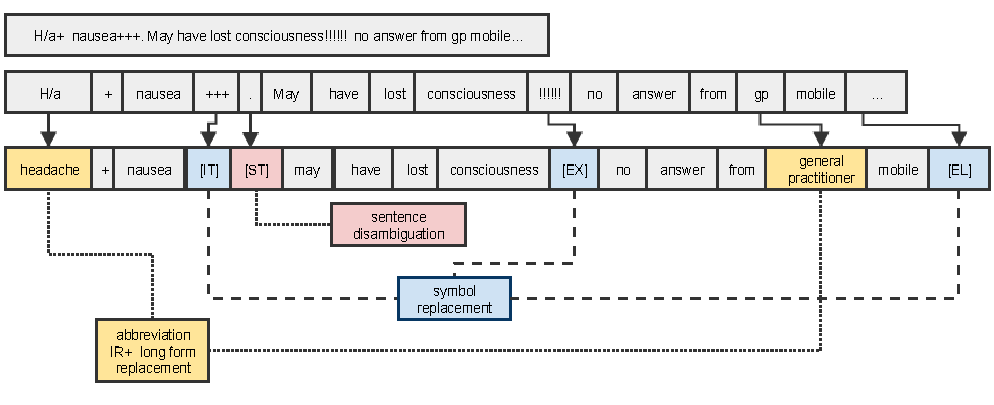
\includegraphics[width=1.0\textwidth]{Figs/scheme-word-replacement.pdf} 

 \caption{Sample FTN text featuring basic symbol replacement}
 \label{fig:word-replacement}
  \end{center}
\end{figure}

\begin{comment}
!!!!!!!!!!!!!!!!!!!!!!!
Similar to twitter 
!!!!!!!!!!!!!!!!!!!!!!!!!!!!!!!!!!!!!!
\end{comment}

\section{Impact on corpus}
\label{section:preproccesing-impact-on-corpus}

So far in this chapter the treatment of the various aspects of the medicinal text has been isolated from the ultimate impact on the dataset as a whole. While the information retrieval, clustering, and transformation methodologies developed to this end have value in themselves, their main relevance within the scope of this thesis is their impact on the ultimate performance of the frequent user classifier.  

This section will provide details on the changes that this preprocessing has affected in relation to the FTN as a whole. While dimensionality reduction was an aim of the preprocessing described in this chapter, this did not mean that data reduction was a goal.

The preprocessing described in this chapter was an iterative process, and the eventual output was guided by initial results provided by ANN architecture testing. As this testing progressed, and it became clearer that a model that could understand patterns relating to the sequence of input (or at least the immediate context of input) was likely to be more successful in classification, the choice was made to include information relating to the preprocessing tasks into the text itself.

By reducing the number of symbol patterns it was hoped that a machine could more easily interpret the intended meaning of such patterns. The same was true for numbers. Instead of having strings of numbers interpreted as unique lexemes, all numbers (integers, real numbers, etc.) would be discretised to a general token representing numerical strings. This is because even machine learning algorithms that could understand textual context would have to see each of these numbers multiple times in the same sort of environments to work out that were, in fact, numbers. Because of the large volume of unique numbers in the dataset, there would be many instances where the machine learning algorithm would inevitably fail to make this connection. While discretising numbers in this fashion was going to lose the scalar data from the FTN, this information was unlikely to ever be useful. While a context like "patient has temperature of 42 C" provides much more value, from a medicinal point of view, than "patient has a temperature of numtoken celsius", there are a vast number of different contexts within which numerical values arise; and these contexts were often not recorded in a particularly consistent manner. For instance the above example could be written: "pt temp 107.6.". 

Relating back to the free-text\index{free-text} data described in Section \ref{section:free-text-description}, the volume of additional data generated by the processes described in this chapter can be seen in Table \ref{table:corpus-preprocessed}, with the change presented in brackets. The change in unpreprocessed text \textbf{P} and preprocessed text \textbf{P'} also shows a significant drop in the number of unique words present in the text. Note that a very large number of the unique lexemes remaining in the corpus are single instance spelling errors. Although it is the contention of this thesis that the steps detailed in this chapter would no doubt support any subsequent attempts to address these spelling errors (as important terms in the form of contractions would be less subject to type two errors in any hypothetical automated spell correction program) the actual development and deployment of such an effort is outside the scope of the preprocessing steps being considered in this chapter.    


\newcommand{\forceindent}{\leavevmode{\parindent=2em\indent}}






\begin{table}[h]
   \ra{1.3}
\caption{Free-text data in preprocessed corpus.}
\label{table:corpus-preprocessed}
\begin{center}
\begin{tabular}{|l|c|c|c|}
\hline
\textbf{attribute}     & \textbf{entries} & $\mathbf{\bar{c}}$ & $\mathbf{\bar{w}}$   \\
\hline
olc\_history   & 15226  & 212.86 (+30.14) & 34.01 (+17.43) \\

olc\_examination & 11326  & 148.13 (+33.13) & 22.65 (+15.41) \\

olc\_diagnosis & 120433  & 36.04 (+10.58)  & 5.13 (+3.47)  \\

olc\_treatment    & 123517  & 122.08 (+47.22)  & 17.11 (+11.5) \\

teleguides & 58906 & 315.17 (+43.89)  & 49.95 (+11) \\
\hline
\end{tabular}
\end{center}
\label{table:free-text}
\end{table}

% Please add the following required packages to your document preamble:
% \usepackage{booktabs}


\begin{table}[ht]
\forceindent
\begin{tabular}{|l|cc|}
\hline
                  & \multicolumn{1}{c}{\textbf{P}} & \multicolumn{1}{c|}{\textbf{P'}} \\  
Unique words      & 131841                         & 114507                           \\
Lexical diversity & 0.072                          & 0.069                            \\ \hline
\end{tabular}

\end{table}


\begin{comment}

\begin{table}[ht]
\begin{tabular}{|r|cc|}
\hline
               & \multicolumn{1}{l}{\textbf{Unique words}} & \multicolumn{1}{l|}{\textbf{Lexical diversity}} \\  
Unpreprocessed & 131841                                      & 0.072                                           \\
Preprocessed   & 114507                                      & 0.069                                           \\ \hline
\end{tabular}
\end{table}


\end{comment}






\section{Summary}


This chapter detailed some of the major steps taken in preprocessing the FTN contained within the corpus. This research is agnostic in relation to potentially encouraging users to improve their methods of recording information in free-text fields. Instead, scalable machine learning approaches have been presented that can automatically process domain specific terms. While accepting that the data contained within FTN were noisy and highly heterogeneous, this chapter attempted to develop means of processing the text that would reduce this noise and heterogeneity while respecting the integrity of the information contained within case notes. Attempting to fix errors and reduce noise, without inadvertently destroying valuable information, is a challenging process; as is evidenced by the methodologies discussed in this chapter. Notwithstanding their impact on the classification processes described in Chapter \ref{chpt:predictive-modelling}, these cleaning and clustering methodologies also have relevance in other medical contexts.   

 \chapter{Predictive Modelling of Frequent Users}
 \label{chpt:predictive-modelling}
  \nomenclature[1]{GRU}{Gated recurrent unit}
 
 
  \newcommand\MyBox[2]{
  \fbox{\lower0.75cm
    \vbox to 1.7cm{\vfil
      \hbox to 1.7cm{\hfil\parbox{1.4cm}{#1\\#2}\hfil}
      \vfil}%
  }%
}
 

\section{Introduction}


















A key objective at this stage of the research is to derive the optimal neural network architecture for the purposes of medical diagnostics within the scope of this thesis. To this end we conducted a series of comparisons between three different types of neural network over a range of parameters and hyperparameters, in relation to the classification of textual notes, and measured the optimal performance of each. The textual notes themselves were presented to each of these classifiers in different data forms in order to ascertain the ideal format for their processing, and whether a marked difference between the different classifiers emerges based upon the format of the data provided to them. 




In order to test our hypothesis that FTN could provide effective features for generating predictive models to determine frequent users, we sought to develop a proof of concept centred upon deep learning methodologies. A number of questions needed to be addressed in relation to the development of an ANN classifier. While ANNs\index{Artificial Neural Networks} have gained considerable attention in recent years, there is no universal design that can be employed, irrespective of domain or data type, that is guaranteed to produce optimal results. Moreover this extends beyond considerations relating to the architecture of the ANN itself, but includes the manner in which data is to be presented to the ANN.  

\hl{The contents of this chapter were in part published in EMBC 2019 `Outlier Detection in Health Record Free-Text Using Deep Learning'} \cite{wallace2019outlier} and `Analysis of EHR Free-text Data with Supervised Deep Neural Networks' \cite{wallace2018analysis} in CSCE 2018 which sought to identify means of successfully classifying frequent user cases using neural networks.

This chapter will describe the measures taken to address these stages of the research: how the data was prepared for classification, how competing ANN architectures performed with FTN data, and how different data implementations affected classifier effectiveness. 

The aim of this section is to provide a key component of a decision support, namely the means to predict patients that are likely to require elevated levels of care. For training purposes, this is defined as any patient who called or was referred to the OOHC\index{Out-of-hours Health Care} in question more than 40 times in a calendar year. \hl{This figure was chosen as a transitory working figure while a more permanent definition of frequent user was obtained in consultation with Caredoc. This figure was adequate in its role in determining a suitable model for case classification.}  

This research used the popular open-source library Tensorflow \index{Tensorflow}1.14.0 \cite{tensorflow2015-whitepaper}, with Python 3.6.6, packaged by conda-forge in the development of the ANN architectures described below. The CUDA API V9 was also used for interfacing with a graphics processing unit for these tests \cite{nvidia2017cuda}. The software these models were built and tested on was compiled with MSC v.1900 64 bit (AMD64).



\section{Architecture Choice}
\label{M}

\subsection{Data Processing}
\label{DP}


In the scope of the investigation conducted by this part of the thesis we excluded all normalised data, such as information relating to the age, or sex of the patient, or information concerning the urgency of or amount of time taken in handling patients' calls. This section exclusively focuses on free-text data, which, notwithstanding  its huge potential in medical analytics, has traditionally been the most difficult source of medical data for use in the context of machine learning. The exclusive aim of this section is to determine the optimal configuration of data and neural network hierarchy for the classification of free-text derived from EHR\index{Electronic Health Record} systems.  

In processing the data we cleaned and tokenised the already anonymised free-text notes (as described in Chapter \ref{chpt:medicial-dataset}).  Cleaning of free-text\index{free-text} included the conversion of unicode to ASCII, the removal of noise (such as the use of symbols to emphasise certain words within the text). We developed our own tokenisation program as our data proved too dissimilar from the data that the majority of off-the-shelf tokenenisers were designed for (e.g. typical Twitter text). Measures that were developed included the disambiguation of words, numbers, and symbols. Where appropriate, symbols and letters which represented words were substituted by their real-world equivalents. As such, a section of text that reads ``temp+++! - 1/2diazepam, tdsx5" would be changed to `` temp ++ 1/2 diazepam , tds * 5". These cleaning and tokenisation processes were designed to be conservative, and were by no means exhaustive in their approach. For instance, within the scope of this section's investigation, no attempt was made to alter the free-text in order to correct spelling errors, disambiguate drug names, or unroll acronyms. Each of the data forms that the free text was converted into (such as word embeddings or list of characters) used this cleaned and tokenised data as its base.

\begin{figure}[htbp]
   \begin{center}

 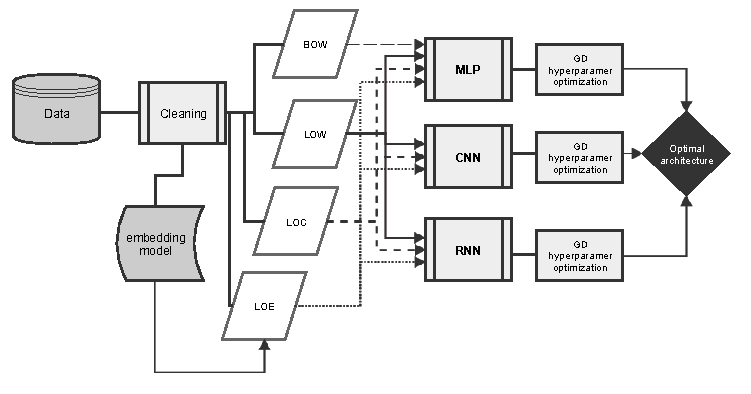
\includegraphics[width=1.0\textwidth]{scheme-lstm1.pdf} 

 \caption{Model for ANN\index{Artificial Neural Networks} testing.}
 \label{fig:ANN-model}
  \end{center}
\end{figure}
 
Data was converted into four mutually exclusive structures: namely bag-of-words (BOW\index{Bag-of-words representation}), list of characters (LOC), list of words (LOW), and list of word embeddings (LOE), as can be seen in Figure \ref{fig:ANN-model}. Each of the data formats has potential merits and demerits in terms of their potential capacity to provide useful representations of patient cases for the purposes of classification. Most of the formats include either implicit or explicit contextual information, with bag-of-words alone being formed of an entirely unstructured representation of patient cases. As mentioned in the related research in Section \ref{section:ANN-(theory)}, bag-of-words is a very popular model for use with this type of task. However, due to its unstructured nature, bag-of-words was only suitable for use in conjunction with the multilayer perceptron ANNs\index{Artificial Neural Networks}. List-of-words and list-of-characters are representations of the data at either a lexeme or character level. Unlike bag-of-words, the structure inherited from the patient cases was maintained. 

FTN attributes (visible in Table \ref{table:free-text}) were appended to one another for each separate case for the generation of input data, as described in Section \ref{section:free-text-description}. Training data was produced using downsampling in order to produce a dataset evenly balanced between positive and negative cases. This approach was necessary in order that domination by a majority class be avoided during training. 

\subsubsection{Length and channels}

To the end of processing FTN\index{free-text} data for use with ANN models this thesis borrows a concept more usually associated with image classification. The term `channel' typically refers to the value (or colour) of an individual pixel being analysed. For the purposes of the FTN data, `channel' refers to the value that the individual token possesses. The actual upshot of this depends on the specific data being considered. In the list-of-characters representation, `channels' relates to the range of ASCII values available. For the BOW\index{Bag-of-words representation} and list-of-words representations, `channels' refers to one-hot encoding of words. Finally, for the word embedding model, `channels' refers to the dimensions of the word embedding. 

It was necessary for reasons of practical consideration to put a fixed upper limit on both the number of channels and the volume of input being examined. For all representations this related to a size of one hundred, for both `channels', and length. In terms of channel number, for both BOW\index{Bag-of-words representation} and list-of-words this correlated to the top one hundred words by frequency in the corpus. For list-of-words, list-of-characters, and list-of-word-embeddings the length of input related to the first one hundred instances of each respective data-type encountered in the associated case FTN. If the input was less than one hundred in length, the input would be padded with zeroes to make up the deficit. If the input was longer than one hundred of its respective data representation, that additional information would be discarded. 

\subsubsection{Word Embeddings}

A significant number of rule-based and statistical language processing algorithms regard
words as atomic symbols. In natural language contexts, such as that found in FTN, this translates to a very sparse representation of the vocabulary. This `one-hot' encoding of lexical information does not document the similarity between any of these symbols. For instance, `chesty' and `wheezing' would from this point of view have no relationship with one another. The practical implication of this is that symbols which appear infrequently are liable to have little impact on algorithmic performance, even if they represent strong information gain. For one thing, even if the particular feature selection technique that is used manages to preserve these data when presenting material to the ML application, their very infrequency would make it less likely for the ML application to have sufficient examples from which to learn these symbols' importance. Moreover, such representations fail to provide information relating to   distributional semantics or co-occurrence statistics. Co-occurrence can be somewhat addressed using N-gram representations. Although N-grams (for instance 2-gram representations) are not considered as part of the testing process in this section, this role is, to all intents and purposes, performed by the LOW representation of the FTN, which essentially preserves co-occurrence information.    

Unsupervised learning using neural networks to create vector based word embeddings has become a very popular means of addressing this particular issue. To this end Word2Vec was used, trained in the manner described in Section \ref{section:word_embeddings}.

%While this approach was necessary, insofar that domination by a majority class had to be avoided during training, this produced a significant prospect for overfitting\index{Overfitting}. 




%How many channels?

\subsection{Hyperparameter optimisation}
\label{section-hyperparemter-optimisation}


  





Choice of hyperparameters can be crucial to the effectiveness of a particular ANN architecture. This becomes a limiting factor due to the fact that suitable hyperparameters may not be known \textit{a priori} \cite{zhou2018exploring,zheng2019hyperparameter}. Unfortunately, choice of hyperparameters is subject to high dimensionality.  Furthermore, tuning of a single hyperparameter may affect the performance of another hyperparameter; therefore tuning in isolation may not necessarily be effective. 

% Please add the following required packages to your document preamble:
% \usepackage{booktabs}






The most simple approach to finding the correct combination of hyperparameters is to perform an exhaustive search across all combinations of hyperparameters. This methodology, known as Grid Search \cite{goodfellow2016deep}, is only suitable within a narrow subset of hyperparamers. Instead, Bayesian optimisation for hyperparameters was performed \cite{snoek2012practical}. Expected improvement can be defined as


\begin{equation}
EIy\textsuperscript{*}(x) = \int_{-\infty}^{y\textsuperscript{*}}(y\textsuperscript{*} -  y)p(y|x)dy
\end{equation}

Where \textit{y}\textsuperscript{*} is a threshold value for the objective function, \textit{y} is the actual value of the objective function, and \textit{p}(\textit{y}|\textit{x}) is the surrogate model.



This model was used to obtain the hyperparameters of hidden layers in relation to the number of layers, number of hidden units, learning rate, activation function, and optimisation function used within each of the three types of ANN. The search space (which is detailed in Table \ref{table:hyperparameter-tuning}) for both RNN\index{Recurrent Neural Network} and CNN\index{Convolutional Neural Networks} featured dropout, while CNN\index{Convolutional Neural Networks} optimisation also included filter, kernel and pool sizes. 

\begin{table}[htbp]

\caption{Search space for hyperparameters.}
\begin{center}
\begin{tabular}{@{}clc@{}}
\cmidrule(r){1-1} \cmidrule(l){3-3}
\textbf{Activation function} & \textbf{} & \textbf{Optimiser} \\ \cmidrule(r){1-1} \cmidrule(l){3-3} 
sigmoid                      &           & Adadelta           \\
hard sigmoid                 &           & Adagrad            \\
relu                         &           & Adam               \\
tanh                         &           & Ftrl               \\
leaky relu                   &           & Gradient Descent   \\ \cmidrule(r){1-1}
                             &           & Momentum           \\ \cmidrule(l){3-3} 
\end{tabular}
\end{center}
\label{table:hyperparameter-tuning}
 \end{table} 

\begin{table}[htbp]
\begin{center}
\begin{tabular}{@{}llc@{}}
\toprule
\textbf{hidden layers}  & \textbf{learning rate}        & \multicolumn{1}{r}{\textbf{dropout}} \\ \midrule
\multicolumn{1}{c}{1-5} & \multicolumn{1}{c}{0.001-1.0} & 0.0-1.0                              \\ \bottomrule
\end{tabular}
\end{center}

\end{table}


\subsection{Long Short-Term Memory}
\label{LSTM}

Long Short-Term Memory (LSTM\index{Long Short-Term Memory}) \cite{gers1999learning}, originally developed to help solve the vanishing gradient problem common in simple RNN\index{Recurrent Neural Network}, is a block that has the capacity to store representations of recent input events. RNN\index{Recurrent Neural Network} have proven application in NLP\index{Natural Language Processing} problems due to capacity of the ANN to remember term dependencies, and could be useful in the interpretation of contextual information in patient cases. As gated units have been proven to be superior to vanilla RNN\index{Recurrent Neural Network}, regardless of context, there was little reason to reestablish this here. A standard LSTM\index{Long Short-Term Memory} unit was implemented, featuring an input gate, an output gate and a forget gate, but the number of LSTM\index{Long Short-Term Memory} units was variable, with the depth to be determined during hyperparameter optimisation.   



\subsection{Selection Outcome}
\label{section-hyperparameter-results}

The output of the classifiers was a binary truth value based on the determined likelihood that the patient case being tested belonged to someone who either currently, or in the near future, would have escalating levels of required care. %A natural issue to arise when 

One hundred different models, based upon different sets of hyperparameters were trained, and ran up to a thousand epochs for each ANN configuration. This experiment was conducted using 45\% of positive cases for training data, 40\% of positive cases for validation data, and 15\% of positive cases for testing data. Training and validation datasets were balanced, while testing used a quarter of the corpus. A total of 3260 cases (or rows) were allocated for training, 2900 cases for validation, and 73584 cases for testing. Testing was conducted using the best configuration, as derived during hyperparameter optimisation.




% Please add the following required packages to your document preamble:
% \usepackage{booktabs}
\begin{table}[htbp]
\centering
\caption{Accuracy results on validation data.}
\begin{tabular}{@{}l|ccc@{}}
\toprule
\textbf{Data}           & \textbf{MLP\index{Multi-Layer Perceptrons}} & \textbf{CNN} & \textbf{RNN\index{Recurrent Neural Network}} \\ \midrule
Bag of Words            & 0.8 $^{\mathrm{a}}$         &            &           \\
List of characters      & 0.64         & 0.72         & 0.73         \\
List of words           & 0.72         & 0.75         & 0.76         \\
List of word embeddings & 0.73         & 0.73         & 0.82         \\ \bottomrule
\multicolumn{4}{c}{}{$^{\mathrm{a}}$Bag of words was used only with MLP}
\end{tabular}
\label{table:hyperparameter-testing}
\end{table}

As shown in Table \ref{table:hyperparameter-testing} above, Multilayer Perceptrons were inferior to both CNN\index{Convolutional Neural Networks} and RNN in relation to contextual information. However, MLP\index{Multi-Layer Perceptrons} performed well using Bag-of-words, underpinning the validity of the frequent usage of this combination, as discussed in Section \ref{section:ANN-(theory)} It was also remarkably fast to train an MLP\index{Multi-Layer Perceptrons} on a simple bag-of-words model, relative to the other models under consideration. 

Character level encoding proved an inferior representation regardless of ANN type. The high dimensionality of feature space was not offset by quality of the data presented to the classifiers, thus generating both long training times and inferior accuracy.

One-hot encoding of lexemes with contextual conservation generated adequate results, and in testing proved the most suitable representation for Convolutional Neural Networks. Although the CNN\index{Convolutional Neural Networks} model achieved good results in all categories, it was nonetheless consistently outperformed by Recurrent Neural Networks using LSTM\index{Long Short-Term Memory}.

\begin{table}[htbp]
\caption{Optimal configuration.}
\begin{center}
\begin{tabular}{|c|c|c|c|c|c|}
\hline


\cline{2-4} 
\textbf{Model} & \textbf{\textit{$\mu$}} & units & layers & $\varphi$ & opt \\
\hline
MLP &  \  0.73639 &  48 &  2 &  leaky relu & GradientDescent  \\
\hline
CNN & 0.002257 & 76 & 3 & relu & Adam   \\
\hline
RNN &0.003186  & 100 & 3 & tanh & GradientDescent   \\ 
\hline
 

\end{tabular}
\label{tab3}
\end{center}
\end{table}




Recurrent Neural Networks using LSTM\index{Long Short-Term Memory} performed well using all data representations. However, the use of word embeddings saw a significant increase in the potential output of this classifier. While significantly more expensive to train than an MLP\index{Multi-Layer Perceptrons} network, this combination was the most successful in classifying patients.


\noindent
\renewcommand\arraystretch{1.5}
\setlength\tabcolsep{0pt}
\begin{table}[htbp]
\caption{Testing results.}
\begin{tabular}{c >{\bfseries}r @{\hspace{0.7em}}c @{\hspace{0.2em}}c @{\hspace{0.7em}}l}
  \multirow{10}{*}{\parbox{1.1cm}{\bfseries\raggedleft actual\\ value}} & 
    & \multicolumn{2}{c}{\bfseries Prediction outcome} & \\
  & & \bfseries p & \bfseries n & \bfseries total 13287 \\
  & p$'$ & \MyBox{443}{} & \MyBox{12844}{} & P$'$ \\[2.2em]
  & n$'$ & \MyBox{108}{} & \MyBox{60189}{} & N$'$ \\
  & total 60297 & P & N &
\end{tabular}
\label{table:LSTM-first-results}
\end{table}

The optimal hyperparameters, listed above in Table \ref{tab3} relate to the Bag-of-Words\index{Bag-of-words representation} model for MLP\index{Multi-Layer Perceptrons}, the List-of-Words model for CNN\index{Convolutional Neural Networks}, and list of word embeddings for LSTM\index{Long Short-Term Memory}. The optimal hyperparameters for CNN\index{Convolutional Neural Networks} included a pool size of 3 and 18 dense units. As the Recurrent Neural Network, with word embeddings, performed best, its results in testing are shown above in the confusion matrix in Table \ref{table:LSTM-first-results}, while the training cost using this configuration is shown in below in Figure \ref{fig1}. A dropout rate of 0.136 was also applied to this network in order to reduce the occurrence of overfitting\index{Overfitting}. Although the results, as described in Table \ref{table:LSTM-first-results}, were at this stage quite modest, the architectural framework for future neural network development within the project had been established.

%Our deep LSTM network achieved precision of 0.82.


\begin{figure}[htbp]
\centerline{\includegraphics[width=3.0in]{training2.png}}
\caption{Training cost for RNN.}
\label{fig1}
\end{figure}


\subsection{Discussion}


This section above detailed not only that ANNs\index{Artificial Neural Networks} can achieve high quality results in classifying patients from medical free-text, but that not all data representations performed as well as one another. A single data representation was likely to produce different results, depending on the type of ANN it was provided to. Moreover, the performance of any given ANN was largely tied to the specific hyperparameters in use. Applying Bayesian optimisation allowed the application of suitable hyperparameters for use with each of the ANNs\index{Artificial Neural Networks}, and as such determine the most suitable ANN for use with the data under consideration. Of course, merely reporting the hyperparameters which gave the optimal performance does not provide the full story. There were numerous combinations of hyperparameters which prevented any successful training of the respective model. Equally there were numerous combinations which performed well, but had marginally weaker results than the set of hyperparamters reported above. As an aside, it is interesting and somewhat surprising how well MLP\index{Multi-Layer Perceptrons} managed to perform with a character level representation of the dataset (bear in mind that with the balanced class representation of the validation data, that 50\% accuracy is no better than random).

While an n-gram representation of characters would be likely to perform better than the individual character representation, character level representations had clearly been the least effective method of representing case data, regardless of the model employed. This data representation was also an order of magnitude more expensive to train compared to other representations.     

Notwithstanding the mixed quality of data, and even in the absence of individual patient histories, the ANN architectures performed well. This was particularly relevant to the research question of this thesis, which concerns the classification of a cohort for whom there is not a well defined set of symptoms. As such, there was no need to attempt to extract potentially useful features for a machine learning algorithm, but rather allow the neural networks to decide which features were deemed most representative.  

Whilst the classifier performed well in determining frequent-user from non frequent-user cases, the issue remained that the so-called black box model of neural networks creates challenges in interpretability \cite{liu2018improving}. The capacity of a classifier to not merely provide the service of identifying members of a cohort, but to inform medical professions the phenotypes likely to represent certain patients is of specific importance within the domain of medical treatment \cite{london2019artificial,preece2018asking}. Therefore a means to potentially identify the salient features of the FTN that contributed to positive and negative predictions became an objective of our research.



As Recurrent Neural Networks with LSTM\index{Long Short-Term Memory} had outperformed the other ANN architectures listed above, many concerns relating to the hand curation of features were allayed. As a sequential architecture, Recurrent Neural Networks have an inherent appreciation of context \cite{yin2017comparative}. Consequently there was no need to process individual lexemes to represent their specific context. For instance, contextual negation did not have to be processed through the NegEx algorithm \cite{chapman2001simple}, as the RNN\index{Recurrent Neural Network} itself could learn the significance of negation. Unlike rare lexemes (like misspelled medication names), these types of contexts were in plentiful supply. This contextual understanding, supplemented with the semantic information contained within the word embedding representation of the corpus, combined to give a comprehensive approach to the NLP\index{Natural Language Processing} context of the FTN.

Nevertheless, numerous questions remained unanswered. Could superior results be achieved by using an alternative gating technique to LSTM\index{Long Short-Term Memory}; by using a different method of word embedding to Word2Vec\index{Word2Vec} trained on the corpus; or by applying the parameterised data of the corpus as input features to the network? Furthermore this section did not test the corpus using the preprocessing techniques described in Chapter \ref{chpt-preprocessing}. The following sections will address these outstanding issues, including whether increasing the input itself (in terms of either length or dimensionality) might improve results.  



\section{Recurrent Neural Network Application}
\label{RNNA}

\subsection{Data selection}
\label{testing-methodologies}

After consultation with the OOHC\index{Out-of-hours Health Care} in question, the two criteria chosen for classifying frequent users were patients who contact the OOHC\index{Out-of-hours Health Care} more than 50 times in a year (approximately once a week), which will be described as high frequent users, and those that contact the OOHC\index{Out-of-hours Health Care} more than 24 times in a year, which are simply described as frequent users. For the sake of brevity, in the following tables, `threshold' will be abbreviated to \textit{t}. As described in Section \ref{section:frequent-users-rr}, this demarcation between different grades of frequent use is fairly typical in the medical domain. Training, test, and validation sets were split by user and contained 50\%, 25\%, and 25\% of positive cases respectively, where training and validation sets were balanced, and testing set imbalanced. Consequently, when conducting experiments considering frequent users, t(24), training used a total of 7,365 cases, validation used 3,682 cases, and testing used 283,289 cases in total. For experiments considering high frequent users t(50), training used a total of 2,922 cases, validation 1,461, and testing 289,953 cases in total. All results discussed from Section \ref{word-embedding-comparrison} to Section \ref{extending-threshold} were obtained using 5-fold cross validated testing sets \cite{arlot2010survey}.    

\subsection{Word embedding comparison}
\label{word-embedding-comparrison}

\begin{figure}[ht]
   \centering
   \begin{tabular}{@{}c@{\hspace{.5cm}}c@{}}
 \includegraphics[page=1,width=1.0\textwidth]{embc0.pdf} & 
   \end{tabular}
 \caption{Case with transformation performed, featuring identification and unrolling of contractions,  and identification and replacement of shorthand. }
 \label{fig:text-transormation-1}
\end{figure}

\begin{figure}[ht]
   \centering
   \begin{tabular}{@{}c@{\hspace{.5cm}}c@{}}
 \includegraphics[page=1,width=1.0\textwidth]{embc1-1.pdf} & 
   \end{tabular}
  \caption{Another case with transformations, showing the identification and replacement of medications with generic varieties. }
 \label{fig:text-transormation-2}
\end{figure}  


Although RNN (more specifically using LSTM) had been determined, through the results of Section \ref{section-hyperparameter-results}, to be the most promising model to classify frequent user cases, some questions concerning the data itself remained. Consequently testing was conducted to verify the efficacy of the preprocessing described in Chapter \ref{chpt-preprocessing}. 

The preprocessing techniques described in Chapter \ref{chpt-preprocessing} were applied to the FTN. Two examples of the final representation of text based upon these processing techniques can be seen in Figure \ref{fig:text-transormation-1} and  \ref{fig:text-transormation-2}. In this unrolling of acronyms and abbreviations, and identification and replacement of textual shorthand e.g. `+++', the specific method used to identify and/or transform contractions are added as a feature in of itself.


The word embedding comparison was to be made in relation to the GloVe\index{GloVe} (or Global Vectors) model, which is trained on the non-zero entries of a global word-word co-occurrence matrix, which tabulates how frequently words co-occur with one another \cite{pennington2014glove}.  The Word2Vec\index{Word2Vec} model, described in Section \ref{section:word_embeddings}, was retrained on this version of the text. Again, the GloVe\index{GloVe} model was also trained on both the unpreprocessed and preprocessed form of the corpus. Finally we compared Word2Vec pre-trained on the Google News corpus (3 billion running words) word vector model (3 million 300-dimension English word vectors).
For each of these embeddings a comparison was made of performance on the corpus both before and after the textual transformations described in Tables \ref{table:embedding-comp-24} and \ref{table:embedding-comp-50}.








It was no great surprise that the word embeddings trained on the Google News corpus had inferior performance to those trained on our corpus, as the register used in clinical notes deviates significantly from standard linguistic formulation. While textual transformations performed concerning the unrolling of acronyms would have improved the accuracy of this model, other textual transformations (like medication reconciliation) wouldn't have had any noticeable impact, while others (like contraction clustering) would likely have had a negative impact on this particular model's performance. 

\begin{table}[ht]

\setlength{\tabcolsep}{9pt}
      \centering
\caption{Performance relating to word embedding method\index{GloVe}: t(24).}
\label{table:embedding-comp-24}
      \resizebox{\columnwidth}{!}{%
\begin{tabular}{@{}lcccccc@{}}
\toprule
                     & \multicolumn{2}{c}{\textbf{Unpreprocessed}} & \multicolumn{2}{c}{\textbf{Preprocessed }} \\ \midrule
            & PPV                  & NPV                  & PPV                 & NPV                 \\
\textit{W2V}          & 0.66$\pm 0.018$ &    0.72$\pm 0.044$&  0.76$\pm 0.034$     & 0.74$\pm 0.04$                    \\
\textit{GloVe}       & 0.64$\pm 0.077$  &   0.75$\pm 0.073$&  0.72$\pm 0.022$     & 0.76$\pm 0.03$                   \\
\textit{Google News} & 0.62$\pm 0.037$  &   0.69$\pm 0.051$&  0.69$\pm 0.043$      & 0.74$\pm 0.05$                    \\ \bottomrule
\end{tabular}
}
\end{table}

\begin{table}[ht]

\setlength{\tabcolsep}{9pt}
      \centering
\caption{Performance relating to word embedding method\index{GloVe}: t(50).}
\label{table:embedding-comp-50}
      \resizebox{\columnwidth}{!}{%
\begin{tabular}{@{}lcccccc@{}}
\toprule
                     & \multicolumn{2}{c}{\textbf{Unpreprocessed}} & \multicolumn{2}{c}{\textbf{Preprocessed }} \\ \midrule
            & PPV                  & NPV                  & PPV                 & NPV                 \\
\textit{W2V}         & 0.81$\pm 0.013$     & 0.82$\pm 0.01$ & 0.85$\pm 0.016$     & 0.85$\pm 0.028$                   \\
\textit{Glove}     & 0.82$\pm 0.022$     & 0.81$\pm 0.019$ & 0.84$\pm 0.026$     & 0.81$\pm 0.022$                  \\
\textit{Google News} & 0.76$\pm 0.026$     & 0.79$\pm 0.009$ & 0.75$\pm 0.037$     & 0.80$\pm 0.016$                   \\ \bottomrule
\end{tabular}
}
\end{table}

Textual transformation of the clinical notes, as seen in Figures \ref{fig:text-transormation-1} and \ref{fig:text-transormation-2}, had a clear positive impact on both  the precision and negative predictive performance of the different models (with the exception of the pretrained model's precision in relation to high frequent users). Note that these transformations are designed primarily to improve classification accuracy, irrespective of human intelligibility. The divergence in performance between the three types of word embeddings used was interesting, but ultimately indicated that Word2Vec\index{Word2Vec} trained on the corpus was the most reliable of those tested.






\subsection{Gating comparison}

Gated Recurrent Units (GRU\index{Gated Recurrent Units}) are a more recent method of implementing gating, relative to LSTM\index{Long Short-Term Memory}, but feature fewer parameters \cite{cho2014learning}. As both architectures looked promising for use in relation to unstructured text \cite{bansal2016ask}, our tests featured a comparison of the performance of these respective  









\newmdenv[bottomline=false]{topbot}
\newmdenv[topline=false]{bottombot}

\begin{landscape}
   \begin{figure*}[tpb]
   
      \centering
      \begin{topbot}

      \includegraphics[page=1,width=0.75\textwidth]{scheme-tensorboard-0(1)(half-0).pdf}
      \end{topbot}
      

   \end{figure*}
\end{landscape}   

\begin{landscape}
   \begin{figure*}[tpb]
   
      \centering
      \begin{bottombot}

      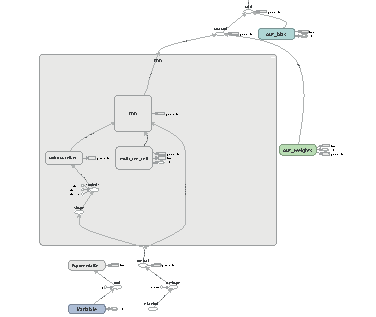
\includegraphics[page=1,width=0.75\textwidth]{scheme-tensorboard-0(1)(half-1).pdf}
      \end{bottombot}
      \caption{Schematic representation of neural network architecture.}
      \label{fig:scheme-tensorboard}
   \end{figure*}
\end{landscape}   

\noindent models. The output of the ANNs\index{Artificial Neural Networks} was a continuous value reflecting the determined likelihood that the case belonged to a frequent user.

\subsubsection{Channel and word length}

Varying the size of channel or input length had not yet been considered as part of ANN testing. While this was an area that merited investigation in its own right, the matter was given particular attention given the effect of preprocessing. Notwithstanding the fact that most significant findings are likely to be written by nurses or doctors at the top of FTN notes, \hl{as elaborated in Section} \ref{section:preproccesing-impact-on-corpus}, the average size of text within FTN\index{free-text} had increased significantly. This heightened the perceived possibility of potentially valuable information being excluded from consideration due to the fixed length of input. Somewhat similarly, testing had not yet excluded the possibility of increased predictive performance by raising the ceiling of dimensionality of word embedding input.  


A further question related to the potential impact that including the parameterised data, described in Section \ref{section:dataset-description}, might have upon the model. The actual means of providing this data to the classifier was predominantly limited to appending this data to the input stream. However, it was hypothesised that providing the model with case data relating to: the age of the patient that the case was related to, the medical card status of the patient, the sex of the patient, the priority ascribed to the case, the time of day that the case had taken place, and the amount of time that the case had lasted might make a significant improvement to the classification accuracy. In counterpoint, the impact of simply adding random values in lieu of these parameterised data was assessed as part of testing. Both parameterised data and noise was prepended to the input stream. 



These series of experiments seemed an ideal venue in which to compare the performance of the LSTM\index{Long Short-Term Memory} and GRU\index{Gated Recurrent Units} gating techniques, and consequently all sets of variables described above were tested against both the LSTM\index{Long Short-Term Memory} and GRU\index{Gated Recurrent Units} models. Both the GRU\index{Gated Recurrent Units} and LSTM\index{Long Short-Term Memory} models were subject to hyperparameter optimisation prior to these experiments (though hyperparamters had already been derived for the LSTM\index{Long Short-Term Memory} model, changes in both the data, and the RNN\index{Recurrent Neural Network} cells that the model was composed of, warranted a fresh round of hyperparameter testing).       


%While dropout was considered as part of the search space of hyperparameters that were subject to Bayesian hyperparameter optimisation (along with the number of layers, learning rate, activation function, and optimisation function used within the ANN), we also sought another potential means to counter overfitting\index{Overfitting}. Our approach was to deliberately prepend the vector data input with noise, to see if this would improve ultimate testing results. This was tested against the addition of normalised features derived from the corpus. Although these normalised features were quite limited in scope, it was hypothesised that the introduction of these features, such as patient age and gender, might improve classification performance. 







%\begin{figure}[htbp]
% \caption{Graph of Recurrent Neural Network featuring LSTM}
%   \begin{center}
%
% 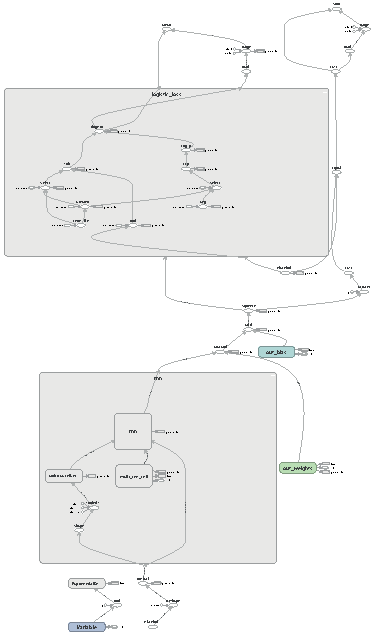
\includegraphics[width=1.14\textwidth]{Figs/scheme-tensorboard-0(1).pdf} 
%
%
% \label{fig:scheme-tensorboard}
%  \end{center}
%\end{figure}







\subsection{Methodology}



Both RNN\index{Recurrent Neural Network} models had batch sizes of 100, while weights were set using He / MRSA initialisation \cite{he2004initialization}. This is different from Section \ref{section-hyperparemter-optimisation} where weights were simply set by a pseudo random number generation. Hyperparameters were again derived using Bayesian optimisation (as described in Section \ref{section-hyperparemter-optimisation}) 


The structure and set of hyperparameters determined through Bayesian optimisation to be the most successful, and used pursuant to the ultimate classification of patients in relation to this chapter, was a Recurrent Neural Network featuring a four layer LSTM\index{Long Short-Term Memory} with a learning rate of 0.001, dropout of 0.3, batch size of 100, and using the Adam optimiser \cite{kingma2014adam}. The alternative Recurrent Neural Network tested featured five layer GRU\index{Gated Recurrent Units}, with learning rate of 0.009, dropout of 0.25, and using the Adagrad optimiser \cite{duchi2011adaptive}. It was uncertain whether increasing the length of input (maximum number of lexemes considered in each case) and channels (the dimensionality of word embeddings) would improve results, and as such, these were also tested. Holdout data related exclusively to cases of patients not featured in training.


\begin{table}[ht]
\caption{Testing hyperparameters.}
\setlength{\tabcolsep}{9pt}
\centering
\resizebox{\textwidth}{!}{%
\begin{tabular}{@{}lcc@{}}
\toprule
                    & \textbf{Long-Short Term Memory} & \textbf{Gated Recurrent Units} \\ \midrule
Learning Rate       & 0.001                           & 0.009                         \\
Number of Layers    & 4                               & 5                             \\
Activation function & relu                            & relu                          \\
Optimiser           & Adam                            & Adagrad                       \\
Dropout             & 0.3                             & 0.25                          \\ \bottomrule
\end{tabular}%
}

\label{table:gating-hyperparameters}
\end{table}



%   \begin{figure}[thpb]
%      \centering
%      \framebox{\parbox{3in}{
%}
%      \includegraphics[scale=0.5]{50-2019-01-26T20}
%      }
%      \caption{ROC curve over FA patients with predicted threshold greater than 49 annual contact events}
%      \label{figurelabel}
%   \end{figure}





\subsection{Results}
\label{section:LSTM-results}


    \begin{figure}[thpb]
      \centering
      \framebox{\parbox{3in}{
}
      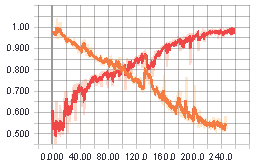
\includegraphics[scale=1.8]{Figs/graph-training-cost.pdf}
      }
      \caption{Training accuracy (red) and cost (orange) of RNN with LSTM modules.}
      \label{graph:training-lstm}
   \end{figure}




LSTM\index{Long Short-Term Memory}, using Word2Vec\index{Word2Vec}, trained on the corpus, and using the hyperparameters described above overall performed strongly when given 100 lexemes of input, coupled with a dimensionality of 100 channels. The following results describe the use of the testing datasets outlined in Section \ref{testing-methodologies}. 

The receiver operating characteristic (ROC) curve and the area under curve (AUC) were used to evaluate the effectiveness of the classifier. The ROC curve shows the trade-off between the true positive rate (TPR) and the false positive rate (FPR), and in particular is robust in the context of class imbalance \cite{japkowicz2011evaluating}. If the ROC curve is closer to the top left corner of the graph, the model is better. The AUC is the area under the curve generated. When the area is closer to 1, the model is better. AUC can be calculated as




\begin{equation}
AUC(f) = \frac{\sum_{i = 1}^{|T_{p}|}(R_i - i)}{|T_p||T_n|}
\end{equation}

Where $T_p \subset T \: and \: T_n \subset T$ are, respectively, the subsets of positive and negative examples in test set T, and $R_i$ is the rank of the \textit{i}th example in $T_p$ given by classifier \textit{f} \cite{japkowicz2011evaluating}.

    \begin{figure}[thpb]
      \centering
      \framebox{\parbox{3in}{
}
      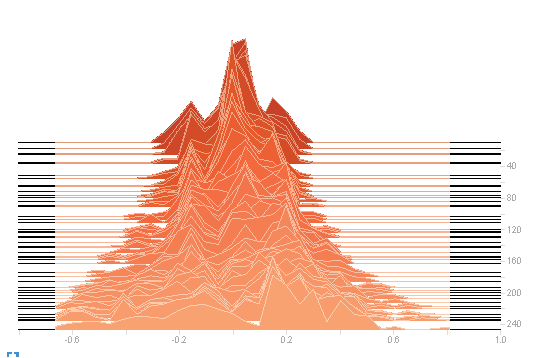
\includegraphics[scale=1.0]{Figs/histogram-tb.pdf}
      }
      \caption{Histogram displaying binned weights of LSTM model, with y-axis relating to step number.}
      \label{fig:histogram-lstm}
   \end{figure}


The hyperparamers of the networks were as defined in Table \ref{table:gating-hyperparameters}. Unless otherwise stated, the models described were tested on the Word2Vec set of word embeddings trained on the preprocessed corpus. 
 
    \begin{figure}[thpb]


      \centering
      \framebox{\parbox{3in}{
}
      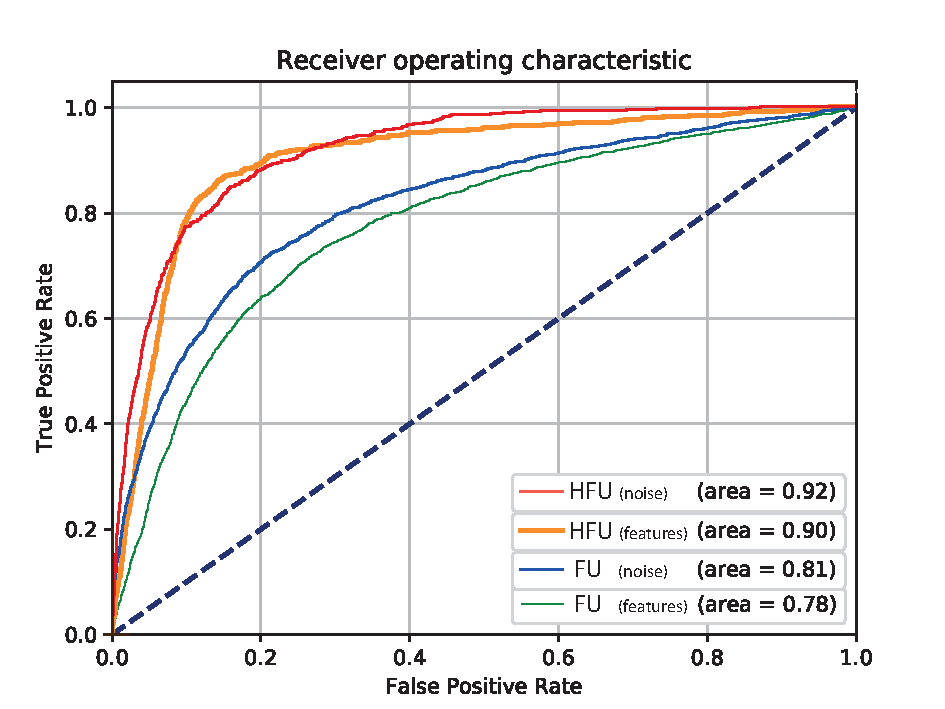
\includegraphics[scale=0.7]{Figs/graph-roc2.pdf}
      }
      \caption{ROC curve over both high frequent user cases and frequent user cases using LSTM.}
      \label{graph:roc-LSTM-noise_vs_features}
   \end{figure}



\begin{comment}
\begin{table*}[h]
   \ra{1.3}
      \centering
      \caption{Architecture and input comparison}
      \label{table:lstm-gru}
      \resizebox{\columnwidth}{!}{%

\begin{tabular}{|lll|ll|ll|ll|ll|}
\hline
   &        &      & \multicolumn{4}{c|}{LSTM}                                                                 & \multicolumn{4}{c|}{GRU\index{Gated Recurrent Units}}                                               \\\cline{4-11}
   &        &     & \multicolumn{2}{c|}{Features}                         & \multicolumn{2}{c|}{Noise}        & \multicolumn{2}{c|}{Features}      & \multicolumn{2}{c|}{Noise}         \\
T  & Length & C   & PPV                                 & NPV             & PPV             & NPV             & PPV             & NPV              & PPV             & NPV             \\ \hline
24 & 100    & 100 & \multicolumn{1}{r}{0.71$\pm 0.006$} & 0.76$\pm 0.005$ & 0.75$\pm 0.033$ & 0.75$\pm 0.047$ & 0.69$\pm 0.067$ & 0.76$\pm 0.01$   & 0.74$\pm 0.035$ & 0.74$\pm 0.035$ \\
24 & 100    & 200 & \multicolumn{1}{r}{0.73$\pm 0.021$} & 0.75$\pm 0.003$ & 0.72$\pm 0.047$ & 0.76$\pm 0.013$ & 0.74$\pm 0.009$ & 0.75$\pm 0.015$  & 0.72$\pm 0.011$ & 0.73$\pm 0.022$ \\
24 & 200    & 100 & 0.71$\pm 0.018$                     & 0.72$\pm 0.012$ & 0.54$\pm 0.21$  & 0.89$\pm 0.081$ & 0.7$\pm 0.014$  & 0.74 $\pm 0.008$ & 0.75$\pm 0.015$ & 0.74$\pm 0.01$  \\
24 & 200    & 200 & \multicolumn{1}{r}{0.78$\pm 0.098$} & 0.63$\pm 0.21$  & 0.38$\pm 0.33$  & 0.91$\pm 0.042$ & 0.78$\pm 0.083$ & 0.63$\pm 0.21$   & 0.67$\pm 0.16$  & 0.82$\pm 0.007$ \\
50 & 100    & 100 & \multicolumn{1}{r}{0.88$\pm 0.009$} & 0.78$\pm 0.008$ & 0.86$\pm 0.012$ & 0.88$\pm 0.014$ & 0.89$\pm 0.015$ & 0.8$\pm 0.013$   & 0.86$\pm 0.023$ & 0.83$\pm 0.027$ \\
50 & 100    & 200 & 0.85$\pm 0.017$                     & 0.83$\pm 0.026$ & 0.88$\pm 0.019$ & 0.84$\pm 0.025$ & 0.78$\pm 0.018$ & 0.89$\pm 0.011$  & 0.81$\pm 0.044$ & 0.86$\pm 0.041$ \\
50 & 200    & 100 & 0.80$\pm 0.083$                      & 0.69$\pm 0.23$  & 0.79$\pm 0.015$ & 0.71$\pm 0.17$  & 0.80$\pm 0.019$ & 0.65$\pm 0.26$   & 0.8 $\pm 0.32$  & 0.83$\pm 0.063$ \\
50 & 200    & 200 & 0.89$\pm 0.048$                     & 0.75$\pm 0.165$ & 0.82$\pm 0.14$  & 0.72$\pm 0.21$  & 0.83$\pm 0.22$  & 0.77$\pm 0.08$   & 0.78$\pm 0.26$  & 0.62$\pm 0.052$ \\
\hline
\end{tabular}%
}
\end{table*}
\end{comment}

\begin{table}
  \setlength{\tabcolsep}{8pt}
\centering
\caption{Architecture and input comparison: LSTM.}
\label{table-lstm}
\begin{tabular}{|lll|ll|ll|} 
\hline
   &        &     & \multicolumn{4}{c|}{LSTM}                                                                      \\ 
\cline{4-7}
   &        &     & \multicolumn{2}{c|}{Features}                           & \multicolumn{2}{c|}{Noise}           \\
T  & Length & C   & PPV                                  & NPV              & PPV              & NPV               \\ 
\hline
24 & 100    & 100 & \multicolumn{1}{r}{0.71$\pm 0.006$ } & 0.76$\pm 0.005$  & 0.75$\pm 0.033$  & 0.75$\pm 0.047$   \\
24 & 100    & 200 & \multicolumn{1}{r}{0.73$\pm 0.021$ } & 0.75$\pm 0.003$  & 0.72$\pm 0.047$  & 0.76$\pm 0.013$   \\
24 & 200    & 100 & 0.71$\pm 0.018$                      & 0.72$\pm 0.012$  & 0.54$\pm 0.21$   & 0.89$\pm 0.081$   \\
24 & 200    & 200 & \multicolumn{1}{r}{0.78$\pm 0.098$ } & 0.63$\pm 0.21$   & 0.38$\pm 0.33$   & 0.91$\pm 0.042$   \\
50 & 100    & 100 & \multicolumn{1}{r}{0.88$\pm 0.009$ } & 0.78$\pm 0.008$  & 0.86$\pm 0.012$  & 0.88$\pm 0.014$   \\
50 & 100    & 200 & 0.85$\pm 0.017$                      & 0.83$\pm 0.026$  & 0.88$\pm 0.019$  & 0.84$\pm 0.025$   \\
50 & 200    & 100 & 0.80$\pm 0.083$                      & 0.69$\pm 0.23$   & 0.79$\pm 0.015$  & 0.71$\pm 0.17$    \\
50 & 200    & 200 & 0.89$\pm 0.048$                      & 0.75$\pm 0.165$  & 0.82$\pm 0.14$   & 0.72$\pm 0.21$    \\
\hline
\end{tabular}
\end{table}


\begin{table}
  \setlength{\tabcolsep}{8pt}
\centering
\caption{Architecture and input comparison: GRU\index{Gated Recurrent Units}.}
\label{table-gru}
\begin{tabular}{|lll|ll|ll|} 
\hline
   &        &     & \multicolumn{4}{c|}{GRU}                                                    \\ 
\cline{4-7}
   &        &     & \multicolumn{2}{c|}{Features}        & \multicolumn{2}{c|}{Noise}           \\
T  & Length & C   & PPV              & NPV               & PPV              & NPV               \\ 
\hline
24 & 100    & 100 & 0.69$\pm 0.067$  & 0.76$\pm 0.01$    & 0.74$\pm 0.035$  & 0.74$\pm 0.035$   \\
24 & 100    & 200 & 0.74$\pm 0.009$  & 0.75$\pm 0.015$   & 0.72$\pm 0.011$  & 0.73$\pm 0.022$   \\
24 & 200    & 100 & 0.7$\pm 0.014$   & 0.74 $\pm 0.008$  & 0.75$\pm 0.015$  & 0.74$\pm 0.01$    \\
24 & 200    & 200 & 0.78$\pm 0.083$  & 0.63$\pm 0.21$    & 0.67$\pm 0.16$   & 0.82$\pm 0.007$   \\
50 & 100    & 100 & 0.89$\pm 0.015$  & 0.8$\pm 0.013$    & 0.86$\pm 0.023$  & 0.83$\pm 0.027$   \\
50 & 100    & 200 & 0.78$\pm 0.018$  & 0.89$\pm 0.011$   & 0.81$\pm 0.044$  & 0.86$\pm 0.041$   \\
50 & 200    & 100 & 0.80$\pm 0.019$  & 0.65$\pm 0.26$    & 0.8 $\pm 0.32$   & 0.83$\pm 0.063$   \\
50 & 200    & 200 & 0.83$\pm 0.22$   & 0.77$\pm 0.08$    & 0.78$\pm 0.26$   & 0.62$\pm 0.052$   \\
\hline
\end{tabular}
\end{table}



It was interesting that the inclusion of features provided no notable improvement in performance by either of the recurrent neural network architectures. In counterpoint, the inclusion of noise had the effect of often reducing the propensity of the classifiers to overfit (which remained an issue, even with dropout). 

The LSTM model was quite closely matched with the performance exhibited by that of the GRU\index{Gated Recurrent Units} model, as can be seen in Table \ref{table-lstm} \hl{and Table} \ref{table-gru} respectively. \hl{It was considered possible that } increasing the length of input or number of channels did not necessarily have any beneficial effect. Even where a higher percentage of true classifications were achieved in one field, there would be a corresponding decrease in true predictions in another. In particular, doubling both input length and channel size tended towards far more unstable models. 




\begin{table}[ht]
\setlength{\tabcolsep}{8pt}
   \ra{1.2}
\centering
\caption{Performance relative to age of frequent user cases.}
\label{table:age-performance}

\begin{tabular}{@{}c|ccc@{}}
\toprule
\textbf{age}           & \textbf{sensitivity} & \textbf{specificity} & \textbf{F1 score} \\ \midrule
\textit{\textgreater90} & 0.65                 & 0.67                 & 0.61              \\
\textit{80-90}         & 0.81                 & 0.77                 & 0.75              \\
\textit{70-80}         & 0.80                 & 0.72                 & 0.81              \\
\textit{60-70}         & 0.78                 & 0.71                 & 0.8               \\
\textit{50-60}         & 0.79                 & 0.7                  & 0.8               \\
\textit{40-50}         & 0.78                 & 0.73                 & 0.84              \\
\textit{30-40}         & 0.75                 & 0.75                 & 0.72              \\
\textit{20-30}         & 0.69                 & 0.76                 & 0.71              \\
\textit{10-20}         & 0.71                 & 0.94                 & 0.52              \\
\textit{\textless10}    & 0.65                 & 0.82                 & 0.61              \\ \midrule
\textbf{all}           & 0.75                 & 0.76                 & 0.76              \\ \bottomrule
\end{tabular}%

\end{table}

A high AUC was achieved for both high frequent users and frequent users with the LSTM model (using 100 channels and 100 input length based on W2V word embeddings trained on preprocessed corpus), visible in Figure \ref{graph:roc-LSTM-noise_vs_features}. The red and orange lines relate to performance for high frequent user cases, with noise or features, respectively. The blue and green lines relate to performance for frequent user cases, with noise or parameterised features, respectively.  High frequent users achieved an AUC of 0.9 (or 0.92 with noise added) and frequent users achieved an AUC of 0.78 (or 0.81 with noise added). 

While these were good results, the lack of impact made by parameterised data on the model's effectiveness was disappointing. Output from the model was also tested as a feature, provided alongside parameterised data, to both RF and SVM in the hope that these algorithms might be able to combine the effectiveness of the ANN's classification of FTN with the information contained within the parameterised data. However, no improvement on the accuracy obtained by the ANN was observed during this evaluation. 


Testing was conducted to ensure that there was no bias towards any particular type of patient. As can be seen in Table \ref{table:age-performance}, based upon validation data of frequent user cases (patients with more than 24 interactions with the OOHC), performance relating to patient age follows almost a standard deviation, with performance strongest at about the mean age of patients, and weakest towards either extreme (those less representative of the cohort as a whole).   

\begin{table}[ht]
\caption{Convolutional Layer Specifications.}
\setlength{\tabcolsep}{9pt}
\centering
\begin{tabular}{@{}lc@{}}
\toprule
     \textbf{Hyperparameter}               & \textbf{Value} \\ \midrule

Convolutional Filters           & 1              \\
Kernel Size      & 5              \\
Pool Size             & 3              \\
Dense Units            & 7                                               \\ \bottomrule
\end{tabular}%

\label{table:cnn-lstm-hyperparameters}
\end{table}



\subsection{Convolutional Layer}



Testing included the implementation of a convolutional layer with the network. CNN-LSTMs are a popular approach to similar domain problems, and can potentially produce improved results \cite{swapna2018automated,shahzadi2018cnn,
li2020hybrid}. A five layer CNN-LSTM was developed (a single convolutional layer on top of a four layer RNN\index{Recurrent Neural Network} featuring LSTM, similar in structure to that depicted in Figure \ref{fig:scheme-tensorboard}) to evaluate potential applicability with the thesis problem. Hyperparameter optimisation identified the specification detailed in Table \ref{table:cnn-lstm-hyperparameters} as best suited to the classifier.

\begin{table}[ht]
\setlength{\tabcolsep}{8pt}
   \ra{1.2}
\centering
\caption{LSTM based Network with Convolutional Layer.}
\label{table:cnn-lstm-results}
\begin{tabular}{@{}lll@{}}
\toprule
\textbf{}                & \textbf{t(24)} & \textbf{t(50)} \\ \midrule
\multicolumn{1}{l|}{PPV} & 0.70$\pm 0.03$         & 0.83 $\pm 0.04$         \\
\multicolumn{1}{l|}{NPV} & 0.82$\pm 0.039$         & 0.84 $\pm 0.02$         \\
\multicolumn{1}{l|}{TPR} & 0.1$\pm 0.01$         & 0.05 $\pm 0.17$         \\
 \bottomrule
\end{tabular}
\end{table}


Again using the testing datasets described in Section \ref{testing-methodologies} we can see that while this convolutional layer increased NPV, and reduced the propensity to overfit, this was achieved with a significant impact to positive case prediction, as shown in Table \ref{table:cnn-lstm-results}.  






\subsection{Overfitting\index{Overfitting}}

Although the model described above provided good results, during training it was clearly exhibiting strong overfitting\index{Overfitting} (visible in Figure \ref{graph:training-lstm} with corresponding updates of weights decreasing over time, visible in Figure \ref{fig:histogram-lstm}). Figure \ref{fig:histogram-lstm} \hl{depicts the rate at which the weights are being adjusted as training occurs, so it is demonstrating quite substantial speed as the weights become mostly adjusted by step 240.} The issue of overfitting was particularly relevant in relation to frequent (as opposed to high frequent) users. Increasing the volume of training examples did not affect this, nor did manually increasing dropout. Although adding noise to the input stream had helped reduce overfitting\index{Overfitting}, the use of weight decay\index{Weight decay} with Adam optimisation was examined as a potential means to improve these results. Weight decay was chosen in lieu of L2 Normalisation, as L2 Normalisation is not effective with adaptive gradient algorithms like Adam \cite{loshchilov2017fixing}.     

\begin{table}[ht]
\setlength{\tabcolsep}{8pt}
   \ra{1.2}
\centering
\caption{LSTM with weight decay.}
\label{table:weight-decay}
\begin{tabular}{@{}c|cccc@{}}
\toprule
    Value         & PPR               & NPR   & TPR     \\ \midrule
\textbf{0.1} & 0.74 $\pm 0.003$  & 0.78$\pm 0.02$ & 0.08$\pm 0.00$ \\
\textbf{0.2} & 0.72  $\pm 0.003$ & 0.79$\pm 0.03$ & 0.08$\pm 0.01$  \\
\textbf{0.3} & 0.73  $\pm 0.004$ & 0.79$\pm 0.04$ & 0.08$\pm 0.01$ \\
\textbf{0.4} & 0.74  $\pm 0.002$ & 0.78$\pm 0.04$ & 0.08$\pm 0.01$   \\
\textbf{0.5} & 0.74  $\pm 0.003$ & 0.81$\pm 0.04$ & 0.09$\pm 0.01$  \\ \
\textbf{0.6} & 0.00                 & 1          & 0.00         \\ \bottomrule
\end{tabular}
\end{table}


Experiments relating to weight decay were performed (visible in Table \ref{table:weight-decay}) with relation to a threshold of 24 cases using the testing dataset described in Section \ref{testing-methodologies} relating to this cohort. This shows that with input and channel length of 100, that for a small penalty to PPR, a statistically significant rise in NPR can be achieved. This was particularly evident with a weight decay of 0.5 (above which the model would tend towards being impossible to train). Although this provided an increase in performance at a threshold of 24 cases, no statistically significant changes were observed with high frequent user cases.

An ROC curve can be observed in Figure \ref{graph:roc-LSTM-weight-decay}, where the black plot represents frequent users, and the red plot, high frequent users.



    \begin{figure}[ht]
      \centering
      \framebox{\parbox{3in}{
}
      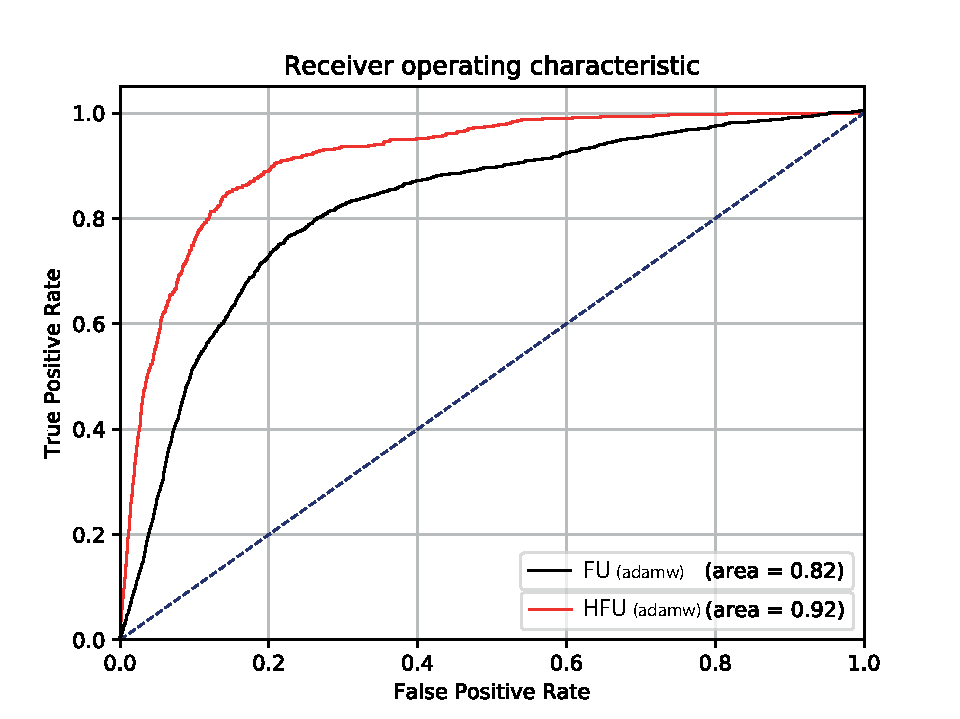
\includegraphics[scale=0.5]{Figs/graph-roc-weightdecay.pdf}
      }
      \caption{ROC curve with LSTM featuring weight decay.}
      \label{graph:roc-LSTM-weight-decay}
   \end{figure}
   
   
       \begin{figure}[ht]
      \centering
      \framebox{\parbox{3in}{
}
      \includegraphics[scale=0.5]{Figs/graph-all-lstm-weightdecay-16threshold.pdf}
      }
      \caption{ROC curve for t(16) patients, with LSTM featuring weight decay.}
      \label{graph:roc-LSTM-16-threshold}
   \end{figure}

\begin{table}[ht]
\setlength{\tabcolsep}{8pt}
   \ra{1.2}
\centering
\caption{Testing on threshold of 16 cases.}
\label{tab:16-cases}
\begin{tabular}{@{}l|cc@{}}
\toprule
             & \textbf{Mean} & \textbf{Stdev} \\ \midrule
\textbf{PPR} & 0.71          & 0.03           \\
\textbf{NPR} & 0.70          & 0.02           \\
\textbf{TPR} & 0.10          & 0.00           \\ \bottomrule
\end{tabular}
\end{table}

\subsection{Extending threshold}
\label{extending-threshold}

The system is configurable regarding the number of calls at which a patient is considered to be a frequent caller. Although outside the scope of what this thesis considers to be a frequent user, to verify that the system's performance is not very sensitive to the threshold number, runs were conducted with patients with a threshold of 16 cases. This almost doubled the number of positive cases being considered (from 7,365 positive cases (\textit{t}(24) to 14,166). As with all other experiments described in Section \ref{RNNA}, a 50\%, 25\%, 25\% split was performed for training, validation, and testing respectively (with training and validation being a balance of positive and negative cases). Consequently 14,166 cases were used for training, 7,083  cases for validation, and 273,087 cases used for testing. The model, although performing consistently well on testing data, as seen in Figure \ref{graph:roc-LSTM-16-threshold}, nonetheless was less accurate than when a higher threshold was considered (seen in Table \ref{tab:16-cases}, over five runs). Note that Figure \ref{graph:roc-LSTM-16-threshold} displays multiple separate runs using the threshold 16 cases, with an average AUC of 0.76. This suggests that characteristics representing frequent users are less strongly exhibited in users with fewer interactions with the OOHC in question.


\subsection{Future Work}

Future work may attempt to build upon the performance of this classification program by finding alternative means to combine structured data with the successful model described in this chapter. Architectural improvements, including regularisation models, may also, hypothetically, prove beneficial. In particular the use of the attention model, though outside the scope of this research, may be used in combination with the LSTM to potentially improve results \cite{deepak2020deep,ma2018sentic,reddy2018predicting}.  





\begin{comment}


Attempts to maximise predictive accuracy and reduce overfitting\index{Overfitting} led to testing involving a combination of LSTM and CNN\index{Convolutional Neural Networks}.   on top of a CNN\index{Convolutional Neural Networks} 

Convolution layer convolve the input using pooling layers, pooling layer helps reduce the representation of input sentences, input parameters, computation in the network and control the overfitting\index{Overfitting} in the network \cite{rehman2019hybrid}. 


\begin{table}[ht]
\setlength{\tabcolsep}{9pt}
\centering
\begin{tabular}{@{}lc@{}}
\toprule
                    & \textbf{CNN-LSTM} \\ \midrule
Learning Rate       & 0.001                                                  \\
Number of Layers    & 4                                                          \\
Activation function & relu                                                      \\
Optimiser           & Adam                                                  \\
Dropout             & 0.3                                                       \\ \bottomrule
\end{tabular}%
\caption{Testing hyperparameters.}
\label{tab:my-table}
\end{table}


\begin{table}[]
\setlength{\tabcolsep}{9pt}
\centering
\caption{}
\label{table:cnn-lstm}
\begin{tabular}{@{}lc@{}}
\textbf{Hyperparameter} & \textbf{Value} \\ \midrule
Learning Rate            & 0.0093         \\
Number of Layers         & 4              \\
Convolutional Filters           & 1              \\
Kernel Size      & 5              \\
Pool Size             & 3              \\
Dense Units            & 7             
\end{tabular}
\end{table}










\end{comment}




\section{Model agnostic discussion}
\label{section:model-agnostic-explanation}





One issue with ANNs\index{Artificial Neural Networks} is their problem of interpretability. In order to improve this aspect of our program, we measured lexemes related to cases based upon whether such lexemes were within cases correctly, or incorrectly, classified by our ANN. Values from the output layer for each case classified was related to the lexemes present within these cases. These values were summed over the whole model for each lexeme, with the count being inversely proportional to how frequent each lexeme was in the corpus as a whole. More formally this can be described as
\begin{equation}
\frac{\sum \Theta_cw}{|w|} c \in C, w \in W
\end{equation}

Where $\Theta$ is the output from the neural network for a given word \textit{w}, in case \textit{c} in the corpus \textit{C}. 





Finally, in accordance with power law distribution \cite{clauset2009power},  only the lexemes which collectively represented 80\% of the entire number of words in the particular dataset were kept in order to reduce the long tail of insignificant lexemes. The resultant graph is visible in Figure \ref{fig-true-results}\footnote{Like most of the images in this thesis, this graph is vector based and should support high magnification when viewed in a digital medium.}.




True positives strongly featured the terms  `depressed', `angina', `suicidal', `gauze', `neuralgia', and `diabetic'. It is worth noting that these terms may often be subject to contextual negation in individual cases (like `patient is not suicidal'). In the case of `suicidal', approximately 25\% of the instances of this term were subject to negation. When considering the course of a patient interaction that results in these terms appearing in free text notes, it is perhaps no surprise that they bear significance, even if they are negated. While words that have strong association with psychological disorders are apparent here (including `anxiety' and `depressed') it is worth noting the terms that also seem to strongly indicate chronic disease (such as `angina', `gauze', and `diabetic'). Both these findings tie in with extant studies which have identified consistent patterns of both chronic and mental illness relating to frequent use \cite{buja2015determines}.

There were also true positive terms that were more surprising, such as `driver', `wondering', and `list'. In particular the term `said' would conventionally seem too frequent to pose much significance. However, the nature of the medical notes is important in this regard. For instance the term `said' appears a total of  2967 times in our corpus, as opposed to 2323 times for a term like `diabetic'. In other textual environments (such as social media) the relative prevalence of two terms like these would be striking. For instance, `said' is contained among the default stopwords for MyISAM search indexes \cite{mysql2019mysql}. 

True negatives for their part were strongly associated with the terms `runny', `viral', `tonsillitis', `tract', and `rash', clearing indicating infections and acute diseases. True negative cases were also strongly connected to family-orientated words, such as `mum', `dad', and `child'. It is worth pointing out that `mum' and `inflamed' also stood out among false negatives. Interestingly, `dementia' and `cancer' were two terms most strongly associated with false positives.   



Looking a bit closer at the distribution of terms relating to incorrect prediction in Figure \ref{fig-false-results}, a far tighter clumping of nodes is apparent. While this may reduce the legibility of some of the node labels, again, like with Figure \ref{fig-true-results} the most important results are those at either end of the spectrum, with the X-axis representing false positives, and the Y-axis representing false negatives. Terms that were strong predictors of both true and false positives also frequently appear in a somewhat similar position in Figure \ref{fig-false-results}. It logically follows that terms which represent strongest information gain for a classifier will also be strongly associated with false predictions when present in those contexts.

There are notable exceptions though. Although `nasal' is a term we did not see appear as strongly associated with correct answers, it is nonetheless closely related to the viral, paediatric based terms we saw in Figure \ref{fig-true-results} so strongly associated with true negatives, and its presence here among false negatives makes sense. However, there are other, more surprising terms related to false negatives. `hand', `bilateral', `talking', `severe', `town', and `nervous' are curious terms to relate to false negatives: particularly `talking' as this was very strongly associated with true positives in  Figure \ref{fig-true-results}.   


   \begin{figure*}[thpb]
   
      \centering
      \framebox{\parbox{2.5in}{
}
      \includegraphics[page=1,width=0.96\textwidth]{network-top12-3.pdf}
      }
      \caption{Undirected graph of co-appearance of strong positive (red) and strong negative (blue) lexemes, with edge weight relative to frequency.}
      \label{fig-top-network}
   \end{figure*}


\begin{landscape}
   \begin{figure*}[thpb]
   
      \centering
      \framebox{\parbox{2.5in}{
}
      \includegraphics[page=1,width=1.8\textwidth]{24THEFULLGRAPH2.pdf}
      }
      \caption{Scatter-plot of the most significant lexemes in cases correctly classified, with the X-axis representing positive predictions, and the Y-axis representing negative predictions.}
      \label{fig-true-results}
   \end{figure*}
\end{landscape}   
   

\begin{landscape}
   \begin{figure*}[]
   
      \centering
      \framebox{\parbox{2.5in}{
}
      \includegraphics[page=1,width=1.8\textwidth]{24THEFULLGRAPH3s.pdf}
      }
      \caption{Scatter-plot of the most significant lexemes in cases incorrectly classified, with the X-axis representing positive predictions, and the Y-axis representing negative predictions.}
      \label{fig-false-results}
   \end{figure*}
\end{landscape} 

A contextual analysis of twelve of the top terms for true positives and true negatives can be seen in Figure \ref{fig-top-network}. This measures occurrence in sentences in all cases, irrespective of whether these cases were correctly classified. Red refers to terms which were strongly associated with true positives, blue with true negatives. Edge weight relates to frequency, while position was generated by the Yifan Hu force-directed graph drawing algorithm \cite{hu2005efficient}.    



Looking at the semantically most similar terms for these lexemes, we get a clear strong connection between some terms, like `throat' and `mum'. Both of these particular terms were strong indicators of true negatives. These two terms despite being very frequent within the corpus, are roughly equivalent to some of the far less frequent terms (like `tonsillitis') in detecting true negatives. True positive terms do not have significantly stronger connections with one another than they do to true-negative terms, based on immediate context at least.

From a word embedding perspective, some of these terms' closest neighbours can be viewed in Table \ref{table:embedding-neighbours}. Note that this is the Word2Vec\index{Word2Vec} model trained on the preprocessed version of the corpus. Though `hand' had a particularly strong association with false-negatives, its word embedding neighbours are surprisingly unremarkable (particularly given the noisy context within which the embedding model was trained).  Inspection of individual frequent user cases with respect to the word `hand' revealed that this word was used in two different contexts: to describe the location of symptoms (e.g. `left hand side' and of course, in relation to injuries to the patients' hands, for instance, as the result of a fall). Again, unusual terms are perhaps conspicuous in their absence in relation to a lexeme such as `said', which has the exact types of semantic neighbours as one would expect (that is to say, apparently generic words relating to communication). However, closer inspection of individual cases shows that the actual act of talking is of significance to some frequent users, who are a cohort more likely to suffer from loneliness and depression \cite{agarwal2019social}.


This testing shows that while lexemes indicating chronic and acute symptoms are important in identifying frequent and non-frequent patients, that both the context, and the particular sequence of words can be of particular significance. Both frequent (e.g. throat) and infrequent (e.g. tonsillitis) terms are significant when considering the role of classification with relation to frequent users.   






\begin{table}[]


      \centering
\caption{Word embedding semantic neighbours.}
\label{table:embedding-neighbours}
\resizebox{\textwidth}{!}{%
\begin{tabular}{|l|lll|}
\hline
\textbf{hand}      & `thumb':0.8670410513877869          & `wrist':0.851659893989563             & `foot':0.833329439163208           \\
\textbf{}          & `forearm':0.8140432834625244        & `elbow':0.7913630604743958            & `arm':0.7791005373001099           \\
\textbf{}          & `fingers':0.77382493019104          & `finger':0.7737174034118652           & `knuckle':0.7483718395233154       \\ \hline
\textbf{bilateral}   & `bilaterally':0.8132901787757874    & `diffuse':0.627751350402832           & `rl':0.5916634798049927            \\
\textbf{}          & `scattered':0.5810911059379578      & `global':0.5810753107070923           & `bialteral':0.5526093244552612     \\
\textbf{}          & `mild':0.5522036552429199           & `bibasal':0.5467664003372192          & `mod':0.5268542766571045           \\ \hline
\textbf{talking}   & `speaking':0.8581299781799316       & `speaks':0.7015131115913391           & `coherent':0.6972201466560364      \\
\textbf{}          & `laughing':0.6873340010643005       & `chatting':0.6761350631713867         & `conscious':0.6636359095573425     \\
\textbf{}          & `calm':0.6479660868644714           & `staring':0.6466795206069946          & `talks':0.6448451280593872         \\ \hline
\textbf{severe}    & `sever':0.769790768623352           & `intense':0.7156710624694824          & `constant':0.6517552733421326      \\
\textbf{}          & `sharp':0.6274532079696655          & `stabbing':0.6245215535163879         & `bad':0.5952492952346802           \\
\textbf{}          & `niggling':0.5927119851112366       & `colicky':0.5842158794403076          & `excruciating':0.5770964622497559  \\ \hline
\textbf{town}      & `hotel':0.5908570885658264          & `north':0.5831862688064575            & `south':0.5829253196716309         \\
\textbf{}          & `base':0.5773507356643677           & `pub':0.5677024126052856              & `hostel':0.558879017829895         \\
\textbf{}          & `park':0.5505035519599915           & `road':0.5482099056243896             & `city':0.5371564030647278          \\ \hline
\textbf{nervous}   & `system':0.6683326959609985         & `trachea':0.6188205480575562          & `TA':0.5814659595489502           \\
\textbf{}          & `neurologically':0.5766158103942871 & `gastrointestinal':0.5764801502227783 & `grossly':0.5526930689811707       \\
\textbf{}          & `peripheral':0.5519363880157471     & `central':0.5334966778755188          & `messaging':0.5289472937583923     \\ \hline
\textbf{driver}    & `receptionist':0.6956810355186462   & `dispatch':0.647824764251709          & `gardai':0.6358491778373718        \\
\textbf{}          & `reception':0.6275129914283752      & `supervisor':0.6190216541290283       & `neighbour':0.5761398673057556     \\
\textbf{}          & `carer':0.5465904474258423          & `pharmacist':0.5379290580749512       & `south':0.5368040800094604         \\ \hline
\textbf{gauze}     & `mepore':0.9428788423538208         & `mefix':0.916340172290802             & `aquacel':0.8925193548202515       \\
                   & `ribbon':0.8817423582077026         & `adaptic':0.8558177351951599          & `melolin':0.8455561995506287       \\
                   & `betadine':0.8319324254989624       & `inadine':0.8264747858047485          & `jelonet':0.8204338550567627       \\ \hline
\textbf{neuralgia} & `postherpetic':0.6631000638008118   & `trigeminal':0.6016533970832825       & `hl':0.4842143654823303            \\
                   & `consultant':0.4773425757884979     & `chiropodist':0.4571322500705719      & `trigeminus':0.45647692680358887   \\
                   & `dietician':0.45278215408325195     & `neuroglia':0.4516264796257019        & `podiatrist':0.450517475605011     \\ \hline
\textbf{viral}     & `virla':0.6982424259185791          & `virall':0.6668179035186768           & `virl':0.6483088731765747          \\
                   & `bacterial':0.6085626482963562      & `herpetic':0.5871016979217529         & `viraemia':0.5690813064575195      \\
                   & `fungal':0.5629815459251404         & `staph':0.5569247007369995            & `streptococcal':0.5457624197006226 \\ \hline
\textbf{said}      & `told':0.7658381462097168           & `stating':0.7619598507881165          & `say':0.7534968852996826           \\
                   & `saying':0.7223905324935913         & `knows':0.7186907529830933            & `says':0.7122293710708618          \\
                   & `thought':0.7096951007843018        & `mentioned':0.7039475440979004        & `advises':0.6869325637817383       \\ \hline
\end{tabular}%
}
\end{table}














\begin{comment}


   
\section{Additional Testing}

It is also the case that, notwithstanding efforts to improve the features derived from such notes, some textual notes have very little data (perhaps a couple of words at most) making the correct classification of these, in isolation, very difficult.

\begin{table}[]
\centering
\setlength{\tabcolsep}{8pt}
\begin{tabular}{cc}
\hline
\textbf{L2 Regularisation} & \textbf{Metric}      \\ \hline
1                          &                      \\
0.8                        &                      \\
0.6                        &                      \\
0.4                        &                      \\
0.2                        &                      \\
-0.2                       & \multicolumn{1}{l}{} \\
-0.4                       & \multicolumn{1}{l}{} \\
-0.6                       & \multicolumn{1}{l}{} \\
-0.8                       & \multicolumn{1}{l}{} \\
-1.0                       & \multicolumn{1}{l}{} \\ \hline
\end{tabular}%

\caption{}
\label{tab:my-table}
\end{table}


%Future work will attempt to build upon the performance of our classification program by finding alternative means to combine structured data with the successful model described in this chapter. Architectural improvements, including regularisation models, may also, hypothetically, prove beneficial.



   
   

\subsection{AdamWOptimizer}

Edit: see also this PR which just got merged into TF.
https://github.com/tensorflow/tensorflow/pull/17438

When using pure SGD (without momentum) as an optimizer, weight decay is the same thing as adding a L2-regularization term to the loss. When using any other optimizer, this is not true.


\end{comment}




\section{Summary}

This chapter detailed the development of a neural network classification system concerning frequent user cases. Several different data types were explored, along with multiple architecture options. This addressed the plurality of architecture types and data formats used in free text classification with relation to neural networks (Section \ref{section:ann-approaches}). When RNNs with word embeddings were identified as the most suitable combination for classifying frequent users, additional tests were run in relation to both these factors: subjecting both the means of preparing word embeddings, and the architecture of the RNN chosen, to a variety of different analyses. These experiments measured the impact of background corpora, of preprocessing, alternative gating techniques, the effects of weight decay, and inclusion of convolutional layers. Finally the performance of the model in relation to a different threshold of patient was examined.  Further tests observed the effects of different calibration methods employed in data preparation, as well as the potential effect of alternative gating approaches. Finally, attempts to explain the model's behaviour with relation to patients both correctly and incorrectly classified were broached, identifying several features from the FTN which pose significance in connection with the cohort being tested.   

 \chapter{Conclusions}
\section{Introduction}
%\subsection{Motivation}

This thesis describes a full pipeline of data mining in relation to an organisation and dataset that has hitherto not been subject to any large scale analytical processes.  The thesis problem of frequent users of OOHC\index{Out-of-hours Health Care} are a difficult cohort for study, owing to their sparsity, disparate demographics, and nonstandardised definition (including an incomplete and inconsistent list of signs and symptoms relating to such patients within medical literature). This concluding chapter will discuss the means used in this thesis to classify cases as belonging to frequent users, the measurement of its achievement, and what future work could potentially be pursued on the foot of this thesis' findings.  




\begin{comment}
\section{Ethical Considerations}

The primary ethical consideration that arises from the research in this thesis is the prospect of a medical care provider theoretically using a system, such as the one described in \ref{}, not for the purposes of early detection of frequent users for intervention and treatment, but rather the opposite: to purposefully exclude these patients from treatment due to the increased level of care that they require, relative to the general population. It is clear that a means of classifying frequent user cases cannot be done in isolation  
\end{comment}



\section{Research Findings and Conclusions}
This section presents the research findings and conclusions with respect to each 
research objective as described in Section \ref{section:thesis-objectives}. \\

\noindent\textbf{The capacity to process raw output from medical systems in such a manner that they can be used in a research capacity.}

One of the more challenging aspects of the research was the treatment of sensitive, real-world data sets stored on live servers of an organisation with limited analytical development. Creating a methodology to extract and clean the high level representation of patient cases was followed by the successful analysis of the data-mart representation of the dataset. This gave a broad overview of a large population of patients, and helped identify potential approaches to patient case classification.\\


\noindent\textbf{Development of machine learning techniques in the context of the domain specific natural language that features within case information.} 

The treatment of medical cases proved the hypothesis that FTN\index{free-text} provided sufficient information to classify patients, despite the noisy context, inconsistent recording practices, and heterogenous data presented within these notes. Somewhat more surprising was that the thesis proved that the parameterised data contained within the corpus was virtually redundant in the face of well processed FTN, at least in the objective of classifying frequent user cases. \\

\noindent \textbf{Domain-sensitive approach to the treatment of medical terms.} 

The thesis presented novel approaches to process medical terms as they might appear in hand-typed free text. These approaches successfully applied textual transformation operations whilst keeping error to a minimum. These approaches were not once-off measures that are exclusively tied to the data set under consideration, but can theoretically be used in any FTN context (provided it is recorded in English). These methodologies have potential application in the context of any historical medical textual data that has been subject to inconsistent recording techniques. \\

\noindent \textbf{Classification of frequent users.} 

This thesis develops a state-of-the-art approach for detecting frequent users in OOHC. This approach requires neither prior background knowledge in relation to the problem definition, nor sophisticated feature extraction techniques on the part of the user when developing training or testing data sets. The model has proven applicability in the course of robust testing and performs well, despite having no access to the previous medical history of any patient it is classifying.     


\section{Medical Application}

The machine learning approaches pursued in this thesis were not developed with the aim of supplanting medical professional's agency, but rather as a diagnostic aid (in much the same way as CDSS\index{Clinical Decision Support Systems} operate). Bearing this in mind, a trade-off had to be established between capturing all relevant cases, and minimising physician input. This trade-off was well represented in the ROC curve, which provides a visual analysis \cite{alpaydin2014introduction} of  the penalty of increased false positives relative to the model's sensitivity.

From an epidemiological point of view the model developed in this thesis provides interventionist recourse but, as is typical for predictive measures for populations, should not be viewed through the lens of base rate fallacy \cite{welsh2012seeing}. The results of the model described in Chapter \ref{chpt:predictive-modelling} are not envisioned as the final word on the patient cases that it classifies, but rather the start of an exploratory process on the part of medical professionals. 

This thesis does not make the claim that the inferences derived in Chapter \ref{section:model-agnostic-explanation} are causal. That is to say, there is no claim that, for instance, depression has a causal effect on patients becoming frequent users. There nonetheless is clear correlation between particular terms and the occurrences of frequent users. This interpretive model provides significant scope for future work where novel patterns may be discovered in  relation to these patients. While this is particularly relevant to frequent users, due to the fact that analysis of patients that become frequent users is an area of active research within public health, there is also the potential to employ these measures for other medical problems.

The research, described in this thesis, has potential for predictive modelling with relation to FTN data. However, it bears repeating that this thesis was able to solve concerns relating to ground truth that usually limits the volume of data available in machine learning applications in the medical domain (as ground truth was related to structured metadata that was automatically generated during the extraction process from Caredoc\index{Caredoc}'s databases, as opposed to being manually curated). Of course it goes without saying that training data was effectively limited by the necessary implementation of downsampling. The model developed showed that a model can achieve notable results when trained with relatively limited data, and successfully used in a real-world context. 



\subsection{Practical Implications}

The use of ANNs for prediction have clear practical implications. These models take significant computing resources to train, and an organisation like Caredoc\index{Caredoc} (or OOHC\index{Out-of-hours Health Care} in general) has little spare hardware for this kind of processing. However, the ANN model developed was ultimately not significantly more demanding than some of the more traditional approaches discussed in Chapter \ref{chpt:machine-learning}. As a point of reference, the final model described in Chapter \ref{chpt:predictive-modelling} takes an average 18 minutes to train using 8.9 * $10^{12}$ floating point operations per second. Moreover, is has been demonstrated in Chapter \ref{chpt:predictive-modelling} that, once trained, the model is able to generalise well with cases of unseen (i.e. holdout) patients. 

%This thesis approaches the difficult task of outlier detection in noisy medicinal medicine. Although the model developed performs well in this task, because of the rare 


\section{Future Work}

This thesis considers a large number of patient interactions over the course of a single year. As such, temporal considerations do not bear a significant role in the analysis performed in this research. However, as discussed in Chapter \ref{chpt:related-research}, research into frequent users' interaction with health care over the course of multiple years is a major area of study. The work described in this thesis could thus be ameliorated through the application of additional data. In particular this would give an opportunity for new types of research.



The most obvious avenue that multiple years' worth of data provides is the prediction of future frequent users (patients that are not initially frequent users, but over a period of time become frequent users). However a more significant contribution could be provided in tandem with interventionist policies. If primary care specialists designed to examine and treat potential frequent users are established, this expanded temporal data could assess the impact, and success or failure, of public health initiatives designed to this end. 

The research described in this thesis also provides an exciting prospect in relation to other medical pathognomonics. This thesis described the classification of outlier patients simply through analysis of what are predominantly telemedical\index{telemedicine} textual notes. However, in a general population the number of people with almost any given disease will be rare \cite{vos2016global}. General primary care records cover very large populations of people, and if downsampling for the detection of an outlier class in the case of frequent users is successfully used with the neural network model described, it follows that this same approach may potentially be used in other contexts. In particular, this invites the detection of unreported or undiagnosed comorbidities. 

The major stumbling block to an investigation of this nature is, as previously stated, based upon the establishment of ground truth. While parametric data was ultimately of little interest in patient case classification in this thesis, it was far from useless as it was used to establish ground truth in the first place (albeit before the extraction from Caredoc\index{Caredoc}'s databases). Similarly, the use of FTN for comorbidity detection or prediction would realistically require one of three resources: parametric data relating to the target disease, diagnostic data relating to these patients held in hospitals or GP surgeries, or manual labelling.

All three approaches pose unique difficulties. However, the use of parametric data may be both the most profitable and cost-efficient method of achieving this goal. For instance, staff in OOHC such as Caredoc\index{Caredoc} could, going forward, record in the normalised parameters provided within the Ad Astra\index{Ad Astra} GUI, any known diseases relating to a patient. This information could then potentially be used for classification with FTN. Using these cases to develop a model, classification of patients as belonging to a particular cohort could be performed, much in the way it is described in this thesis. As shown in this thesis, this type of classification can be successfully performed using only a single case in relation to a given patient. Consequently this provides a potential way to help quickly identify hitherto unknown morbidities in a large population. More exciting still is that a system of this kind, once trained, would not need parameterised recording of patient diseases in order to perform classification (though the absence of such would naturally preclude initial large-scale assessment of performance). 




%\include{Chapter-7/chapter7}




% ********************************** Back Matter *******************************
% Backmatter should be commented out, if you are using appendices after References
%\backmatter

% ********************************** Bibliography ******************************
\begin{spacing}{0.9}

% To use the conventional natbib style referencing
% Bibliography style previews: http://nodonn.tipido.net/bibstyle.php
% Reference styles: http://sites.stat.psu.edu/~surajit/present/bib.htm

%\bibliographystyle{apalike}
\bibliographystyle{unsrt} % Use for unsorted references  
%\bibliographystyle{plainnat} % use this to have URLs listed in References
\cleardoublepage
\bibliography{References/references} % Path to your References.bib file


% If you would like to use BibLaTeX for your references, pass `custombib' as
% an option in the document class. The location of 'reference.bib' should be
% specified in the preamble.tex file in the custombib section.
% Comment out the lines related to natbib above and uncomment the following line.

%\printbibliography[heading=bibintoc, title={References}]


\end{spacing}

% ********************************** Appendices ********************************

\begin{appendices} % Using appendices environment for more functunality

%!TEX root = ../thesis.tex
% ******************************* Thesis Appendix A ****************************
\chapter{}

%\subsubsection{Ethical Approval}


   \begin{figure*}[hpb]
   
      \centering
      \framebox{\parbox{2.5in}{
}
      \includegraphics[page=1,width=0.92\textwidth]{Figs/Ethics-Application.pdf}
      }
     
      \label{figurelabel}
   \end{figure*}
   
   
\begin{table}[]
\setlength{\tabcolsep}{8pt}
   \ra{1.2}
\centering
\caption{Pharmaceutical context stopword list}
\label{table:app-stopwords}
\begin{tabular}{|lllll|}
\hline
a   & at   & has & its  & to   \\
an  & be   & he  & of   & was  \\
and & by   & in  & on   & were \\
are & for  & is  & that & will \\
as  & from & it  & the  & with \\ \hline
\end{tabular}
\end{table}




\begin{table}[]
\setlength{\tabcolsep}{8pt}
   \ra{0.8}
\centering
\caption{Pharmaceutical context stopword list}
\label{table:app-contractions}
\begin{tabular}{@{}lllllllll@{}}
pns   & ani   & da    & aero  & hm    & lsa   & pmum  & reson & vvs   \\
poabs & anle  & db    & aert  & hn    & lsasy & pmxh  & respi & wg    \\
poss  & ano   & dd    & afce  & hoem  & lsat  & pn    & respo & wh    \\
resps & anout & dl    & afeeb & hoeme & lsb   & pn.if & respt & wl    \\
sm    & ansc  & dn    & afert & hof   & lscp  & pnad  & ress  & wo    \\
sti   & antb  & dob   & aft   & hogh  & lscss & pnail & ressp & wram  \\
tb    & antip & dod   & aga   & hoh   & lsd   & pnc   & rf    & wre   \\
ts    & anu   & ds    & agai  & hoi   & lse   & pno   & rft   & wrg   \\
ul    & anx   & du    & agan  & hoid  & lsee  & pnr   & rh    & wrgh  \\
wb    & anyt  & dv    & agao  & hoids & lsf   & pnrtl & rhs   & wrghh \\
aa    & ao    & dw    & agi   & hoigh & lsft  & pnt   & ri    & wrst  \\
aal   & aok   & ea    & agin  & hoih  & lside & pnu   & rl    & wrt   \\
aay   & aove  & ee    & agoi  & hoild & lsij  & pnv   & rn    & wrye  \\
ab.to & ap    & eo    & agos  & hoim  & lsike & pnx   & ro    & wuh   \\
abbo  & apht  & epu   & agp   & hoime & lsion & po.bd & rp    & xd    \\
abc   & apl   & fd    & agqo  & hoip  & lsit  & po.gp & ru    & xmtvi \\
abcd  & apo   & ferer & agres & hp    & lso   & po.on & rw    & xr    \\
abck  & appl  & ferom & aho   & hsp   & lsore & po.px & sb    & xreps \\
abcss & appx  & feron & aicd  & hu    & lsos  & poa   & sd    & xrock \\
abdd  & apray & ferq  & aice  & hz    & lsot  & poab  & sf    & xrs   \\
abg   & aprt  & ferw  & ain   & ib    & lspin & poaed & sg    & yd    \\
abi   & apts  & fes   & ainly & ibd   & lsr   & poain & sij   & zb    \\
abido & apyr  & fesh  & aj    & ic    & lsser & poale & soc   & am    \\
aboce & aq    & feso  & aja   & io    & lu    & poly  & std   & asop  \\
abofe & aqnd  & fess  & aka   & ip    & luts  & polyc & stg   & bid   \\
abovr & aqpp  & fest  & akert & ivp   & lw    & polys & sts   & cs    \\
abpm  & ar    & feswl & akle  & jd    & mcs   & pom   & sv    & cvid  \\
abso  & arae  & fet   & alc   & jj    & mf    & pomh  & svt   & dvn   \\
absob & aran  & feta  & aldi  & jl    & mk    & pomhx & ta    & echo  \\
abt   & arash & fetac & aletr & ko    & mn    & pon   & tcp   & fast  \\
acei  & ast   & fetec & alkso & lc    & mos   & pone  & tf    & ha    \\
ach   & av    & fetor & alle  & le    & mrt   & porta & ti    & ho    \\
achte & aw    & fett  & alos  & lj    & mv    & porte & tidx  & im    \\
aci   & bc    & fette & alow  & lll   & mw    & posat & tj    & me    \\
acj   & bf    & fev   & alrt  & llq   & nbi   & posay & tl    & ms    \\
ack   & bh    & feve  & als   & lm    & nc    & posdt & tp    & oh    \\
acni  & bk    & fevef & altb  & lo    & nk    & posft & tpp   & or    \\
actv  & bt    & feven & am.is & lom   & nl    & posin & tpr   & os    \\
aday  & bw    & fhhr  & amau  & lrh   & nm    & posit & tpsr  & pa    \\
adb   & bx    & fi    & ambo  & lri   & nv    & posn  & ub    & pop   \\
adbd  & ce    & fmf   & ambu  & lrib  & nvdc  & posr  & uc    & pt    \\
adha  & cf    & fp    & ami   & lrica & nw    & posrt & ud    & rip   \\
adice & ci    & fr    & aml   & lring & odx   & possi & ue    & salt  \\
adj   & coc   & ftr   & amm   & lrit  & oo    & pp    & uo    & sc    \\
adked & ctl   & ftt   & amn   & lrq   & ooc   & ppt   & uq    & sob   \\
adls  & cu    & ga    & amne  & lrrti & ou    & ptr   & ur    & ss    \\
adm   & cvvs  & gc    & amog  & lrs   & ow    & pvd   & usa   & tv    \\
admin & cvz   & ger   & ampk  & lrt   & pb    & pw    & usi   & us    \\
adppt & cwcw  & gf    & amunt & lrte  & pd    & qv    & ut    & va    \\
adr   & cwh   & gh    & anat  & lrtil & pid   & rb    & utu   & vs    \\
adrs  & cwn   & gpn   & anb   & lrtis & pivd  & rc    & ux    & we    \\
adt   & cws   & gr    & ancer & lrtri & pmr   & resh  & vc    & wruh  \\
adyas & cxal  & gs    & andfv & lrtu  & pms   & resi  & vd    & xn    \\
adys  & cxall & hd    & aneak & lrtui & pmsh  & reslt & vq    & xreq  \\
aeds  & cxaps & hfm   & anf   & lryti & pmshx & reso  & vr    &       \\
aeh   & cxase & hh    & anfdd & lrz   & pmt   & resol & vv    &      
\end{tabular}
\end{table}
%!TEX root = ../thesis.tex
% ******************************* Thesis Appendix B ********************************

\chapter{Data Structure}






\begin{table}[]
\centering
\caption{}
\label{tab:my-table}
\begin{tabular}{lc}
\hline
attribute                                   & description                             \\ \hline
Forname                                     & anonymised                              \\
Surname                                     & anonymised                              \\
DOB                                         & dd/mm/yyyy partially anonymised to year \\
Sex                                         & boolean                                 \\
Medical\_Card                               & structured                              \\
ID\_Case\_Entry\_Date                       & date-time                               \\
Case\_No                                    & integer                                 \\
Appointment\_Time                           & inoperative/unreliable                  \\
Relationship\_to\_Caller                    & unstructured                            \\
PriorityOnReception                         & structured                              \\
PriorityAfterAssessment                     & structured                              \\
Cons\_Start\_Date                           &                                         \\
Cons\_End\_Date                             &                                         \\
Consult\_Type                               & structured                              \\
Cons\_Time\_Taken                           &                \\
Consult\_Type                               & structured                              \\

\textbf{OLC\_History}      & free-text                                         \\
\textbf{OLC\_Examination}  & free-text                                         \\
\textbf{OLC\_Diagnosis}    & free-text                                         \\
\textbf{OLC\_Treatment}    & free-text                                         \\
\textbf{Teleguides\_Notes} & free-text                                        
\end{tabular}
\end{table}


\begin{figure}[!t]
\centering
\includegraphics[width=4.0in]{Figs/table-caredoc.png}
% where an .eps filename suffix will be assumed under latex, 
%% and a .pdf suffix will be assumed for pdflatex; or what has been declared
 \DeclareGraphicsExtensions.
\caption{Sample view of Caredoc internal database}
\label{fig:internal-caredoc}
\end{figure}

\end{appendices}

% *************************************** Index ********************************
\printthesisindex % If index is present

\end{document}
